
%% bare_conf.tex
%% V1.3
%% 2007/01/11
%% by Michael Shell
%% See:
%% http://www.michaelshell.org/
%% for current contact information.
%%
%% This is a skeleton file demonstrating the use of IEEEtran.cls
%% (requires IEEEtran.cls version 1.7 or later) with an IEEE conference paper.
%%
%% Support sites:
%% http://www.michaelshell.org/tex/ieeetran/
%% http://www.ctan.org/tex-archive/macros/latex/contrib/IEEEtran/
%% and
%% http://www.ieee.org/

%%*************************************************************************
%% Legal Notice:
%% This code is offered as-is without any warranty either expressed or
%% implied; without even the implied warranty of MERCHANTABILITY or
%% FITNESS FOR A PARTICULAR PURPOSE! 
%% User assumes all risk.
%% In no event shall IEEE or any contributor to this code be liable for
%% any damages or losses, including, but not limited to, incidental,
%% consequential, or any other damages, resulting from the use or misuse
%% of any information contained here.
%%
%% All comments are the opinions of their respective authors and are not
%% necessarily endorsed by the IEEE.
%%
%% This work is distributed under the LaTeX Project Public License (LPPL)
%% ( http://www.latex-project.org/ ) version 1.3, and may be freely used,
%% distributed and modified. A copy of the LPPL, version 1.3, is included
%% in the base LaTeX documentation of all distributions of LaTeX released
%% 2003/12/01 or later.
%% Retain all contribution notices and credits.
%% ** Modified files should be clearly indicated as such, including  **
%% ** renaming them and changing author support contact information. **
%%
%% File list of work: IEEEtran.cls, IEEEtran_HOWTO.pdf, bare_adv.tex,
%%                    bare_conf.tex, bare_jrnl.tex, bare_jrnl_compsoc.tex
%%*************************************************************************

% *** Authors should verify (and, if needed, correct) their LaTeX system  ***
% *** with the testflow diagnostic prior to trusting their LaTeX platform ***
% *** with production work. IEEE's font choices can trigger bugs that do  ***
% *** not appear when using other class files.                            ***
% The testflow support page is at:
% http://www.michaelshell.org/tex/testflow/



% Note that the a4paper option is mainly intended so that authors in
% countries using A4 can easily print to A4 and see how their papers will
% look in print - the typesetting of the document will not typically be
% affected with changes in paper size (but the bottom and side margins will).
% Use the testflow package mentioned above to verify correct handling of
% both paper sizes by the user's LaTeX system.
%
% Also note that the "draftcls" or "draftclsnofoot", not "draft", option
% should be used if it is desired that the figures are to be displayed in
% draft mode.
%
\documentclass[conference]{IEEEtran}
% Add the compsoc option for Computer Society conferences.
%
% If IEEEtran.cls has not been installed into the LaTeX system files,
% manually specify the path to it like:
% \documentclass[conference]{../sty/IEEEtran}





% Some very useful LaTeX packages include:
% (uncomment the ones you want to load)


% *** MISC UTILITY PACKAGES ***
%
%\usepackage{ifpdf}
% Heiko Oberdiek's ifpdf.sty is very useful if you need conditional
% compilation based on whether the output is pdf or dvi.
% usage:
% \ifpdf
%   % pdf code
% \else
%   % dvi code
% \fi
% The latest version of ifpdf.sty can be obtained from:
% http://www.ctan.org/tex-archive/macros/latex/contrib/oberdiek/
% Also, note that IEEEtran.cls V1.7 and later provides a builtin
% \ifCLASSINFOpdf conditional that works the same way.
% When switching from latex to pdflatex and vice-versa, the compiler may
% have to be run twice to clear warning/error messages.






% *** CITATION PACKAGES ***
%
\usepackage{cite}
% cite.sty was written by Donald Arseneau
% V1.6 and later of IEEEtran pre-defines the format of the cite.sty package
% \cite{} output to follow that of IEEE. Loading the cite package will
% result in citation numbers being automatically sorted and properly
% "compressed/ranged". e.g., [1], [9], [2], [7], [5], [6] without using
% cite.sty will become [1], [2], [5]--[7], [9] using cite.sty. cite.sty's
% \cite will automatically add leading space, if needed. Use cite.sty's
% noadjust option (cite.sty V3.8 and later) if you want to turn this off.
% cite.sty is already installed on most LaTeX systems. Be sure and use
% version 4.0 (2003-05-27) and later if using hyperref.sty. cite.sty does
% not currently provide for hyperlinked citations.
% The latest version can be obtained at:
% http://www.ctan.org/tex-archive/macros/latex/contrib/cite/
% The documentation is contained in the cite.sty file itself.






% *** GRAPHICS RELATED PACKAGES ***
%

\ifCLASSINFOpdf
   \usepackage[pdftex]{graphicx}
  % declare the path(s) where your graphic files are
   \graphicspath{{../pdf/}{../jpeg/}{../png/}}
  % and their extensions so you won't have to specify these with
  % every instance of \includegraphics
  \DeclareGraphicsExtensions{.pdf,.jpeg,.png}
  \usepackage[justification=centering]{caption}
\else
  % or other class option (dvipsone, dvipdf, if not using dvips). graphicx
  % will default to the driver specified in the system graphics.cfg if no
  % driver is specified.
  \usepackage[dvips]{graphicx}
  % declare the path(s) where your graphic files are
  \graphicspath{{../eps/}}
  % and their extensions so you won't have to specify these with
  % every instance of \includegraphics
  \DeclareGraphicsExtensions{.eps}
\fi

\ifCLASSOPTIONcompsoc 
\usepackage[caption=false,font=normalsize,labelfont=sf,textfont=sf]{subfig} 
\else \usepackage[caption=false,font=footnotesize]{subfig} 
\fi
% graphicx was written by David Carlisle and Sebastian Rahtz. It is
% required if you want graphics, photos, etc. graphicx.sty is already
% installed on most LaTeX systems. The latest version and documentation can
% be obtained at: 
% http://www.ctan.org/tex-archive/macros/latex/required/graphics/
% Another good source of documentation is "Using Imported Graphics in
% LaTeX2e" by Keith Reckdahl which can be found as epslatex.ps or
% epslatex.pdf at: http://www.ctan.org/tex-archive/info/
%
% latex, and pdflatex in dvi mode, support graphics in encapsulated
% postscript (.eps) format. pdflatex in pdf mode supports graphics
% in .pdf, .jpeg, .png and .mps (metapost) formats. Users should ensure
% that all non-photo figures use a vector format (.eps, .pdf, .mps) and
% not a bitmapped formats (.jpeg, .png). IEEE frowns on bitmapped formats
% which can result in "jaggedy"/blurry rendering of lines and letters as
% well as large increases in file sizes.
%
% You can find documentation about the pdfTeX application at:
% http://www.tug.org/applications/pdftex





% *** MATH PACKAGES ***
%
\usepackage[cmex10]{amsmath}
% A popular package from the American Mathematical Society that provides
% many useful and powerful commands for dealing with mathematics. If using
% it, be sure to load this package with the cmex10 option to ensure that
% only type 1 fonts will utilized at all point sizes. Without this option,
% it is possible that some math symbols, particularly those within
% footnotes, will be rendered in bitmap form which will result in a
% document that can not be IEEE Xplore compliant!
%
% Also, note that the amsmath package sets \interdisplaylinepenalty to 10000
% thus preventing page breaks from occurring within multiline equations. Use:
%\interdisplaylinepenalty=2500
% after loading amsmath to restore such page breaks as IEEEtran.cls normally
% does. amsmath.sty is already installed on most LaTeX systems. The latest
% version and documentation can be obtained at:
% http://www.ctan.org/tex-archive/macros/latex/required/amslatex/math/





% *** SPECIALIZED LIST PACKAGES ***
%
\usepackage{algorithm}
\usepackage{algorithmic}
\renewcommand{\algorithmicrequire}{\textbf{Input:}} 
\renewcommand{\algorithmicensure}{\textbf{Output:}}
% algorithmic.sty was written by Peter Williams and Rogerio Brito.
% This package provides an algorithmic environment fo describing algorithms.
% You can use the algorithmic environment in-text or within a figure
% environment to provide for a floating algorithm. Do NOT use the algorithm
% floating environment provided by algorithm.sty (by the same authors) or
% algorithm2e.sty (by Christophe Fiorio) as IEEE does not use dedicated
% algorithm float types and packages that provide these will not provide
% correct IEEE style captions. The latest version and documentation of
% algorithmic.sty can be obtained at:
% http://www.ctan.org/tex-archive/macros/latex/contrib/algorithms/
% There is also a support site at:
% http://algorithms.berlios.de/index.html
% Also of interest may be the (relatively newer and more customizable)
% algorithmicx.sty package by Szasz Janos:
% http://www.ctan.org/tex-archive/macros/latex/contrib/algorithmicx/




% *** ALIGNMENT PACKAGES ***
%
%\usepackage{array}
% Frank Mittelbach's and David Carlisle's array.sty patches and improves
% the standard LaTeX2e array and tabular environments to provide better
% appearance and additional user controls. As the default LaTeX2e table
% generation code is lacking to the point of almost being broken with
% respect to the quality of the end results, all users are strongly
% advised to use an enhanced (at the very least that provided by array.sty)
% set of table tools. array.sty is already installed on most systems. The
% latest version and documentation can be obtained at:
% http://www.ctan.org/tex-archive/macros/latex/required/tools/


%\usepackage{mdwmath}
%\usepackage{mdwtab}
% Also highly recommended is Mark Wooding's extremely powerful MDW tools,
% especially mdwmath.sty and mdwtab.sty which are used to format equations
% and tables, respectively. The MDWtools set is already installed on most
% LaTeX systems. The lastest version and documentation is available at:
% http://www.ctan.org/tex-archive/macros/latex/contrib/mdwtools/


% IEEEtran contains the IEEEeqnarray family of commands that can be used to
% generate multiline equations as well as matrices, tables, etc., of high
% quality.


%\usepackage{eqparbox}
% Also of notable interest is Scott Pakin's eqparbox package for creating
% (automatically sized) equal width boxes - aka "natural width parboxes".
% Available at:
% http://www.ctan.org/tex-archive/macros/latex/contrib/eqparbox/





% *** SUBFIGURE PACKAGES ***
%\usepackage[tight,footnotesize]{subfigure}
% subfigure.sty was written by Steven Douglas Cochran. This package makes it
% easy to put subfigures in your figures. e.g., "Figure 1a and 1b". For IEEE
% work, it is a good idea to load it with the tight package option to reduce
% the amount of white space around the subfigures. subfigure.sty is already
% installed on most LaTeX systems. The latest version and documentation can
% be obtained at:
% http://www.ctan.org/tex-archive/obsolete/macros/latex/contrib/subfigure/
% subfigure.sty has been superceeded by subfig.sty.



%\usepackage[caption=false]{caption}
%\usepackage[font=footnotesize]{subfig}
% subfig.sty, also written by Steven Douglas Cochran, is the modern
% replacement for subfigure.sty. However, subfig.sty requires and
% automatically loads Axel Sommerfeldt's caption.sty which will override
% IEEEtran.cls handling of captions and this will result in nonIEEE style
% figure/table captions. To prevent this problem, be sure and preload
% caption.sty with its "caption=false" package option. This is will preserve
% IEEEtran.cls handing of captions. Version 1.3 (2005/06/28) and later 
% (recommended due to many improvements over 1.2) of subfig.sty supports
% the caption=false option directly:
%\usepackage[caption=false,font=footnotesize]{subfig}
%
% The latest version and documentation can be obtained at:
% http://www.ctan.org/tex-archive/macros/latex/contrib/subfig/
% The latest version and documentation of caption.sty can be obtained at:
% http://www.ctan.org/tex-archive/macros/latex/contrib/caption/




% *** FLOAT PACKAGES ***
%
%\usepackage{fixltx2e}
% fixltx2e, the successor to the earlier fix2col.sty, was written by
% Frank Mittelbach and David Carlisle. This package corrects a few problems
% in the LaTeX2e kernel, the most notable of which is that in current
% LaTeX2e releases, the ordering of single and double column floats is not
% guaranteed to be preserved. Thus, an unpatched LaTeX2e can allow a
% single column figure to be placed prior to an earlier double column
% figure. The latest version and documentation can be found at:
% http://www.ctan.org/tex-archive/macros/latex/base/



%\usepackage{stfloats}
% stfloats.sty was written by Sigitas Tolusis. This package gives LaTeX2e
% the ability to do double column floats at the bottom of the page as well
% as the top. (e.g., "\begin{figure*}[!b]" is not normally possible in
% LaTeX2e). It also provides a command:
%\fnbelowfloat
% to enable the placement of footnotes below bottom floats (the standard
% LaTeX2e kernel puts them above bottom floats). This is an invasive package
% which rewrites many portions of the LaTeX2e float routines. It may not work
% with other packages that modify the LaTeX2e float routines. The latest
% version and documentation can be obtained at:
% http://www.ctan.org/tex-archive/macros/latex/contrib/sttools/
% Documentation is contained in the stfloats.sty comments as well as in the
% presfull.pdf file. Do not use the stfloats baselinefloat ability as IEEE
% does not allow \baselineskip to stretch. Authors submitting work to the
% IEEE should note that IEEE rarely uses double column equations and
% that authors should try to avoid such use. Do not be tempted to use the
% cuted.sty or midfloat.sty packages (also by Sigitas Tolusis) as IEEE does
% not format its papers in such ways.





% *** PDF, URL AND HYPERLINK PACKAGES ***
%
%\usepackage{url}
% url.sty was written by Donald Arseneau. It provides better support for
% handling and breaking URLs. url.sty is already installed on most LaTeX
% systems. The latest version can be obtained at:
% http://www.ctan.org/tex-archive/macros/latex/contrib/misc/
% Read the url.sty source comments for usage information. Basically,
% \url{my_url_here}.





% *** Do not adjust lengths that control margins, column widths, etc. ***
% *** Do not use packages that alter fonts (such as pslatex).         ***
% There should be no need to do such things with IEEEtran.cls V1.6 and later.
% (Unless specifically asked to do so by the journal or conference you plan
% to submit to, of course. )


% correct bad hyphenation here
\hyphenation{op-tical net-works semi-conduc-tor}


\begin{document}
%
% paper title
% can use linebreaks \\ within to get better formatting as desired
\title{\emph{Taking One Small Step Forward:}\\Finding Low-Frequency Items in Data Streams}


% author names and affiliations
% use a multiple column layout for up to three different
% affiliations

% conference papers do not typically use \thanks and this command
% is locked out in conference mode. If really needed, such as for
% the acknowledgment of grants, issue a \IEEEoverridecommandlockouts
% after \documentclass

% for over three affiliations, or if they all won't fit within the width
% of the page, use this alternative format:
% 
%\author{\IEEEauthorblockN{Michael Shell\IEEEauthorrefmark{1},
%Homer Simpson\IEEEauthorrefmark{2},
%James Kirk\IEEEauthorrefmark{3}, 
%Montgomery Scott\IEEEauthorrefmark{3} and
%Eldon Tyrell\IEEEauthorrefmark{4}}
%\IEEEauthorblockA{\IEEEauthorrefmark{1}School of Electrical and Computer Engineering\\
%Georgia Institute of Technology,
%Atlanta, Georgia 30332--0250\\ Email: see http://www.michaelshell.org/contact.html}
%\IEEEauthorblockA{\IEEEauthorrefmark{2}Twentieth Century Fox, Springfield, USA\\
%Email: homer@thesimpsons.com}
%\IEEEauthorblockA{\IEEEauthorrefmark{3}Starfleet Academy, San Francisco, California 96678-2391\\
%Telephone: (800) 555--1212, Fax: (888) 555--1212}
%\IEEEauthorblockA{\IEEEauthorrefmark{4}Tyrell Inc., 123 Replicant Street, Los Angeles, California 90210--4321}}




% use for special paper notices
%\IEEEspecialpapernotice{(Invited Paper)}




% make the title area
\maketitle


\begin{abstract}
%\boldmath
With the explosive growth of the amount of data and the rapid development of information technology, low-frequency items in data streams have attracted much attention due to their large amount and the rich information contained in them. However, as far as we know, there is no method finding low-frequency items in data streams. To address this problem, we propose an one-pass algorithm, called \emph{BFSS}, which can find the items in a data stream whose frequency is no more than a user-specified support approximately. \emph{BFSS} is simple and has small memory footprints. Although the output is approximate, we can guarantee no false negatives (\emph{FNs}) and only a few false positives (\emph{FPs}) exist in the result. Given a little modification, \emph{BFSS} can be extended to \emph{SBFSS}, which can handle data streams in limited and small space and guarantee only a few \emph{FPs} and theoretically bounded number of \emph{FNs} exist in the result. Experimental results on real-world dataset show \emph{BFSS} achieves high performance using much less space compared to \emph{nCount} and \emph{rCount}, which are two naive methods finding low-frequency items in data streams. \emph{SBFSS} outperforms \emph{lCount}, a method finding low-frequency items in data streams using limited space with a simple replacement strategy, in both precision and recall.
\end{abstract}
% IEEEtran.cls defaults to using nonbold math in the Abstract.
% This preserves the distinction between vectors and scalars. However,
% if the conference you are submitting to favors bold math in the abstract,
% then you can use LaTeX's standard command \boldmath at the very start
% of the abstract to achieve this. Many IEEE journals/conferences frown on
% math in the abstract anyway.

% no keywords




% For peer review papers, you can put extra information on the cover
% page as needed:
% \ifCLASSOPTIONpeerreview
% \begin{center} \bfseries EDICS Category: 3-BBND \end{center}
% \fi
%
% For peerreview papers, this IEEEtran command inserts a page break and
% creates the second title. It will be ignored for other modes.
\IEEEpeerreviewmaketitle



\section{Introduction}
% no \IEEEPARstart
In many real-world applications, information such as web click data \cite{IEEEexample:webdata}, stock ticker
data \cite{IEEEexample:stockticker,IEEEexample:stockticker2}, sensor network data \cite{IEEEexample:sensor}, phone call records \cite{IEEEexample:phonecall}, and network packet traces \cite{IEEEexample:packet} appears in the form of data streams. Motivated by the above applications, researchers started working on novel algorithms for analyzing data streams. Problems studied in this context include approximate frequency moments \cite{IEEEexample:frequencymoments}, distinct values estimation \cite{IEEEexample:distinctestimation,IEEEexample:distinctvalues}, bit counting \cite{IEEEexample:bitcounting}, duplicate detection \cite{IEEEexample:sbf,IEEEexample:duplicatedetec}, approximate quantiles \cite{IEEEexample:quantile}, wavelet based aggregate queries \cite{IEEEexample:wavelet}, correlated aggregate queries \cite{IEEEexample:correlated}, frequent elements \cite{IEEEexample:frequent1,IEEEexample:frequent2,IEEEexample:frequent3,IEEEexample:ldsketch} and top-$k$ queries \cite{IEEEexample:spacesaving,IEEEexample:top-k1}. However, to the best of our knowledge, there is no algorithm finding low-frequency items in data streams. In fact, low-frequency items in data streams have attracted much attention because of the rich information they contain which can be seen through the formulas of entropy of data streams \cite{IEEEexample:metropy}. We take one small step forward to find low-frequency items in data streams approximately in this paper.   
% You must have at least 2 lines in the paragreaph with the drop letter
% (should never be an issue)

\begin{figure}
	\centering
	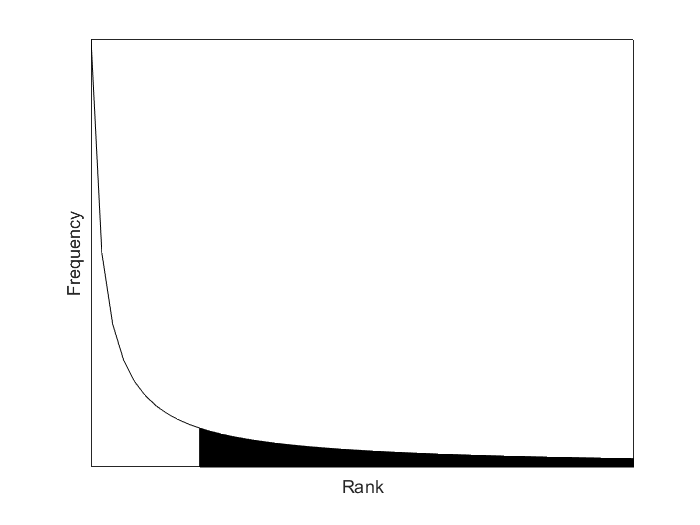
\includegraphics[width=2.5in]{png/zipf.png}
	\caption{Rank-frequency distribution}
	\label{fig:sim}
\end{figure}


\subsection{Motivating Examples}
\subsubsection{Long-Tail Keywords mining}
Long-tail keywords are longer and more specific keyword phrases that visitors are more likely to use when they're closer to a point-of-purchase, the searching frequencies of which are much lower than normal keywords. They're a little bit counter-intuitive, at first, but they can be hugely valuable if you know how to use them.\par
Take this example: if you're a company that sells classic furniture, the chances are that your pages are never going to appear near the top of an organic search for ``furniture'' because there's too much competition (this is particularly true if you're a smaller company or a startup). But if you specialize in, say, contemporary art-deco furniture, then keywords like ``contemporary Art Deco-influenced semi-circle lounge'' are going to reliably find those consumers looking for exactly that product.\par
Long-tail keywords are valuable for businesses who want their content to rank in organic Google searches, but they're potentially even more valuable for advertisers running paid search marketing campaigns. That's because when you bid on long-tailed keywords, the cost per click is inevitably lower, since there's less competition. By targeting longer, more specific long-tail keywords in your AdWords campaigns, you can get higher ad rankings on relevant searches without having to pay a premium for every click. The trick is to find a reliable, renewable source of long-tail keywords that are right for you and for your niche, and a basic premise is their searching frequencies should be low enough to avoid fierce competition, therefore how to effectively find low-frequency items in the related searching streams is necessary.  
\subsubsection{Rare demands mining}
With the rapid development of internet, we can shop and search whatever we are interested in online. Our demands, for example, buying a regular water glass online or searching the information about a tourist attraction etc, are popular most of the time and these demands can be easily satisfied. However, we are no longer satisfied with these popular demands nowadays. For example, it is not so easy for us to buy embroidery stitches or to find the information about a nameless village in China online, because they are rare demands.\par
Microsoft lags so far behind Google in the search engine market because it focused a lot on the head of the queries and didn't acknowledge the long tail, said Yusuf Mehdi, senior vice president of the Online Audience Group for Microsoft Bing, at Search Engine Strategies\footnote{http://www.eweek.com/c/a/Search-Engines/Microsoft-Ignored-the-Long-Tail-in-Search-Bing-Boss-Says-396023}. For Microsoft, focusing on the head instead of the ``long tail'' means that it returned popular queries but failed to satisfy less common queries, the frequencies of which were very low. The long tail of queries ended up yielding more sizable traffic and therefore more money for Google over the last 11-plus years.\par 
From above, we can see that rare demands, in some sense, are more important than popular demands. However, it will consume much space and time to find those less common queries if we store all query items, so it is necessary to design an efficient algorithm to find low-frequency items in data streams.


\subsubsection{Distribution estimation}\label{distribution estimation}
Distribution is a basic property of a data stream, therefore it is important to estimate the distribution of a data stream efficiently. Sampling is a simple and fast method to estimate distributions, however, it may cause significant errors sometimes. Fig.\ref{fig:sim} is a power-law graph, being used to demonstrate the ranking of frequencies of items in data streams under power-law distributions\footnote{the distributions of a wide variety of physical, biological, and man-made phenomena are approximately power-law distributions}. From Fig.\ref{fig:sim}, we observe that low-frequency items have a great influence on distributions, and combining the information of both frequent and low-frequency items, we can have a relatively more comprehensive estimation of the distribution of a data stream.\par 
In fact, \emph{BFSS} can approximately find both frequent and low-frequency items in data streams, given a little modification, \emph{BFSS} can be extended to estimate the percentage of the total frequencies of a certain proportion of items in data streams, for example, we can approximately estimate the percentage of the total frequencies of the most frequent twenty\footnote{``twenty'' is just an example, and the specific value varies and will be explained later} percent of items in a data stream, which is similar to the expression of the famous Pareto principle, also known as the 80-20 rule.

\subsection{Our Contributions}
We are the first to pose and formally define the problem $s$\emph{-Bounded Low-Frequency Elements ($s$-BLFE)}, the formal definition of which will be given later, and to the best of our knowledge, there is no method solving the problem till now.\par

We propose \emph{BFSS}, which extends the classic algorithm \emph{Space Saving} to maintain both frequent and low-frequency items in a data stream approximately. The basic idea of our solution is as follows: each item in a data stream is either a frequent one or a low-frequency one once the threshold $s[\in (0,1)]$ is confirmed, so we can maintain low-frequency items by filtering the frequent items out. A major problem we have to deal with is to maintain an itemset, items in which appear in the data stream, and this can be done approximately using a Bloom filter. \emph{BFSS} gurantees no false negatives and provably few false positives using small memory footprints.\par

However, the size of a Bloom filter must increase with the alphabet's size in order to keep low false positive rate, and here comes a problem: In many embedded devices, such as sensors and routers etc., the storage space is limited and small, in which case \emph{BFSS} will produce many \emph{FPs}. Inspired by the method presented in \cite{IEEEexample:sbf}, we propose \emph{SBFSS} which extends \emph{BFSS} to deal with data streams in limited and small space, and \emph{SBFSS} gurantees a few false positives and theoretically bounded number of false negatives.\par

\subsection{Roadmap}
In Section 2, we present problem statement and some backgrounds on the existing approches which deal with the problem $\epsilon$\emph{-Deficient Frequent Elements}. Our solutions are presented and discussed in Section 3. In Section 4, we experimentally evaluate our methods. Conclusions are given in Section 5.

\section{PRELIMINARIES}
This section presents problem statement and some representative algorithms solving $\epsilon$\emph{-Deficient Frequent Elements} \cite{IEEEexample:sticky} which will be formally defined below. Table \ref{tab:list} summarizes the major notations in this paper.

\begin{table}
	
    \caption{Major Notations Used in the Paper.}
   
	\begin{tabular}{ll}
		\hline	Notation  & Meaning\\ 
		\hline
		\emph{BFSS} & Our first algorithm\\
		\emph{SBFSS} & Our second algorithm\\	
		$S$ & The input data stream\\
		$A$ & The alphabet of $S$\\
		$M$ & The size of $A$\\
		$n$ & The number of distinct items in $S$\\
		$s$ & The user-specified support parameter\\
	    $\epsilon$ & The user-specified error parameter\\
		$D$ & The synopsis used in \emph{BFSS} and \emph{SBFSS}\\
	    $e$ & The item monitored in $D$\\
	    $f(e)$ & The estimated frequency of $e$\\
	    $\Delta(e)$& The estimated error of $f(e)$\\
		$E$ & The item set monitored in $D$\\
		$min$ & The minimum value of $f(e)$ in $D$\\
		$C$ & The maximum number of counters in $D$\\
		$m$ & The number of counters used in $D$\\
		$N$ & The length of $S$\\
		$H$ & The number of hash functions used in \emph{BFSS} and \emph{SBFSS}\\
		$f_S(e)$ & The Frequency of item $e$ in $S$\\ 
		\emph{FPs} &The items in $S$ with frequency more than $\lfloor sN\rfloor$\\& wrongly output\\
		\emph{FNs} & The items in $S$ with frequency no more than $\lfloor sN\rfloor$ \\&wrongly neglected\\
		\emph{BF}  &The Bloom filter used in \emph{BFSS}\\
		$K$ & The size of \emph{BF}\\
		$p_1$ & The percentage of the number of the items \\&whose frequency is above $\lfloor sN\rfloor$\\
		$p_2$ & The percentage of the total frequencies of the items \\&whose frequency is above $\lfloor sN\rfloor$\\
       \emph{SBF} &The Stable Bloom filter used in \emph{SBFSS}\\
        $K'$ & The size of \emph{SBF}\\
        $k$  &  Number of cells used in \emph{SBF}\\
        $d$  & Number of bits allocated per cell\\
        $max$ & The value a cell is set to\\
        $P$ &  Number of cells we pick to decrement by 1 in each iteration\\
        $p$ &  The probability that a cell is picked to be decremented by 1 \\
        &in each iteration\\
        $p'$ &  The probability that a cell is set in each iteration\\
        $W$ & The real data set we used in our experiments\\
       \hline
	\end{tabular}
\label{tab:list}

\end{table}

\subsection{Problem Statement}
Consider an input stream $S = e_1,e_2,..., e_N$ of current length $N$, which arrives item by item. Let each item $e_i$ belong to a universe set $A=\{a_1,a_2,...,a_M\}$ of size $M$.\par
The problem $s$-\emph{BLFE} can be stated as follows: given a data stream $S$ along with two user-specified parameters: a support parameter $s[\in (0,1)]$ and an error parameter $\epsilon[\in (0,1)]$ such that $\epsilon\leq s$.\par
At any point of time, with a small bounded memory, output a list of items with the following guarantees: 
\begin{enumerate}
\item[1.] all items whose true frequency is no more than $\lfloor sN\rfloor$ are output.
\item[2.] no item whose true frequency is no less than $\lfloor sN\rfloor+\lfloor\epsilon N\rfloor$ is output.
\end{enumerate}\par
Imagine a user who is interested in identifying all items whose frequency is no more than $0.1\%N$. Then $s=0.1\%$. The user is free to set $\epsilon$ to whatever she feels is a comfortable margin of error. As a rule of thumb, she could set $\epsilon$ to one-tenth or one-twentieth the value of $s$ and use our algorithm. Let us assume she chooses $\epsilon=0.01\%$ (one-tenth of $s$). As per Property 1, all items with frequency no more than  $0.1\%N$ will be output, there will be no false negatives. As per Property 2, no element with frequency no less than $\lfloor sN\rfloor+\lfloor\epsilon N\rfloor$ will be output.\par

\subsection{Related Work}
As far as we know there is no related algorithm addressing $s$-\emph{BLFE}, however, the methods we propose are based on the algorithm solving $\epsilon$\emph{-Deficient Frequent Elements} which can be described as follows: given an input stream $S$ of current length $N$ and a support threshold $s\in(0,1)$, return the items whose frequency is guaranteed to be no smaller than $\lfloor(s-\epsilon)N\rfloor$ deterministically or with a probability of at least $1-\delta$, where $\epsilon\in(0,1)$ is a user-defined error and $\delta\in(0,1)$ is a probability of failure, so we examine several algorithms solving $\epsilon$\emph{-Deficient Frequent Elements}.\par
Research can be divided into two groups: \emph{counter-based} techniques and \emph{sketch-based} techniques.\par

\textbf{Counter-Based Techniques} keep an individual counter for each item in the monitored set, a subset of A. The counter of a monitored item, $e_i$, is updated when $e_i$ occurs in the stream. If there is no counter kept for the observed ID, it is either disregarded, or some algorithm-dependent action is taken.\par

Two representative algorithms \emph{Sticky Sampling} and \emph{Lossy Counting} were proposed in \cite{IEEEexample:sticky}. The algorithms cut the stream into rounds, and they prune some potential low-requency items at the edge of each round. Though simple and intuitive, they suffer from zeroing too many counters at rounds’ boundaries, and thus, they free space before it is really needed. In addition, answering a frequent elements query entails scanning all counters.\par

The algorithm \emph{Space Saving} , the one we are based at, was proposed in \cite{IEEEexample:spacesaving}. The algorithm maintains a synopsis which keeps all counters in an order according to the value of each counter's monitoring frequency plus maximum possible error. For a non-monitored item, the counter with the smallest counts, \emph{min}, is assigned to monitor it, with the items monitoring frequency $f(e)$ set to 1 and its maximal possible error $\Delta(e)$ set to \emph{min}. Since $min\leq\epsilon N$ (this follows because of the choice of the number of counters), the operation amounts to replacing an old, potentially infrequent item with a new, hopefully frequent item. This strategy keeps the item information until the very end when space is absolutely needed, and it leads to the high accuracy of \emph{Space-Saving}. Experiments done in \cite{IEEEexample:overview_vldbj,IEEEexample:overview} showed \emph{Space-Saving} outperformed other Counter-Based techniques in recall and precision tests.\par

\textbf{Sketch-Based Techniques} do not monitor a subset of items, rather provide, with less stringent guarantees, frequency estimation for all items using bitmaps of counters. Usually, each item is hashed into the space of counters using a family of hash functions, and the hashed-to counters are updated for every hit of this item. Those “representative” counters are then queried for the item frequency with less accuracy, due to hashing collisions.\par

The \emph{Count-Min Sketch} algorithm of Cormode and Muthukrishnan \cite{IEEEexample:count-min} maintains an array of $d\times w$ counters, and pairwise independent hash functions $h_j$ map items onto $[w]$ for each row. Each update is mapped onto $d$ entries in the array, each of which is incremented. The Markov inequality is used to show that the estimate for each $j$ overestimates by less than $n/w$, and repeating $d$ times reduces the probability of error exponentially.\par

The \emph{hCount} algorithm was proposed in \cite{IEEEexample:hcount}. The data structure and algorithms used in \emph{Count-Min Sketch} and \emph{hCount} shared the similarity, but were simultaneously and independently investigated with different focuses.

\section{OUR ALGORITHMS}
In this section, we will discuss our approaches \emph{BFSS} and \emph{SBFSS} in detail.
\subsection{Challenges of $s$-BLFE}
$s$\emph{-BLFE} has two main challenges due to the different features between frequent items and low-frequency items over data streams.\par

\textbf{The Long Tails in data streams}. It can be easily proved that there are at most $\lceil1/s\rceil$ frequent items whose frequency is more than $\lfloor sN\rfloor$ in any data stream, however, there is no upper bound of the number of the low-frequency items whose frequency is no more than $\lfloor sN\rfloor$. In fact, our experiments show that the low-frequency items occupy most of the distinct items in data streams, and it is almost impossible to maintain all of them in memory. Another observation is their frequencies are very low and close as well, and it may consume much space to separate low-frequency items from frequent items especially when $s$ is very small.\par

\textbf{Unpredictability}. A basic and common idea of \emph{Counter-Based Techniques} is to discard potential infrequent items dynamically, and it is based on the fact that potential infrequent items will never become frequent items if they don't appear afterwards, however, this fact no longer applies to low-frequency items in data streams because frequent items will possibly become low-frequency items if they don't appear afterwards. The unpredictability of low-frequency items makes it difficult to maintain them directly.

\subsection{The BFSS Algorithm}\label{sec:bfss}
In consideration of the challenges in $s$\emph{-BLFE}, we tried to solve the problem indirectly by filtering frequent items out which is the underlying idea of \emph{BFSS}.\par
Two algorithms are proposed for updating and outputting results separately. Algorithm \ref{alg:bfss} maintains a Bloom filter $BF$ of size $K$ with $H$ uniformly independent hash functions $\{h_1(x),...,h_H(x)\}$ and a synopsis $D$ with $C$ counters. Each of these $H$ hash function maps an item from $A$ to $[0,...,K-1]$. Initially each bit of BF is set to 0 and $D$ has $C$ empty counters. Each newly arrived item in the stream is mapped to $H$ bits in BF by the $H$ hash functions and we set the $H$ bits to 1. Then if we observe an item that is monitored in $D$, we just increment $f(e)$. If we observe an item, $e_{new}$, that is not monitored in $D$, handle it depending on whether there is an empty counter in $D$. If there is one, we just allocate it to $e_{new}$ and set $f(e_{new})$ to 1 and set $\Delta(e_{new})$ to 0. Otherwise, we just replace the item that currently has the least hits, $min$, with $e_{new}$. Assign $f(e_{new})$ the value $min+1$ and assign $\Delta(e_{new})$ the value $min$.\par

\begin{algorithm}[h]
	\caption{BFSS Update Algorithm}
	\label{alg:bfss}
\begin{algorithmic}[1]
	\REQUIRE Stream $S$, support threshold $s$
	\STATE $N=0,m=0,C=\lceil 1/\epsilon\rceil,K=\lambda',H=\mu'$; \COMMENT{$N$: the length of the input stream; $m$: the number of counters used in $D$; $C$: the maximum number of counters in $D$; $K$: size of Bloom filter; $H$: the number of hash functions; The value of $\lambda'$ and $\mu'$ will be discussed in detail later.}
	\STATE The form of the counters in $D$ is $(e,f(e),\Delta(e))$
	\FOR{$i=0$ to $K-1$}
	\STATE $BF[i]=0$
	\ENDFOR
	\FOR{each item $e$ of stream $S$}
	\FOR{$i=1$ to $H$}
	\STATE $BF[h_i(e)]=1$
	\ENDFOR
	\IF{$e$ is monitored in $D$}
	\STATE $f(e)=f(e)+1$;
	\ELSIF{$m<C$}
	\STATE Assign a new counter $(e,1,0)$ to it
	\STATE $m=m+1$
	\ELSE
	\STATE Let $e_m$ be the item with least hits, $min$
	\STATE Replace $e_m$ with $e$ in $D$
	\STATE $f(e)=min+1,\Delta(e)=min$
	\ENDIF
	\STATE $N=N+1$;
	\ENDFOR
\end{algorithmic}
\end{algorithm}

Algorithm \ref{alg:output} checks and outputs the items whose frequency is no more than $sN$. For each item in $A$, we first check whether it is in $BF$. If the item is not in $BF$, it must not be a low-frequency item. If the item is in $BF$ but not in $D$, we output it as a low-frequency item. If the item appears both in $BF$ and $D$, we identify it as a low-frequency item if $f(e)\leq\lfloor sN\rfloor+\Delta(e)$ with high probability. The time requirement of Algorithm \ref{alg:output} is linear to the range of universe. It is acceptable when the frequency of the requests is not high. 

\begin{algorithm}[h]
	\caption{BFSS Query Algorithm}
	\label{alg:output}
	\begin{algorithmic}[1]
		\REQUIRE \emph{BF}, $D$, $s$, $A$, $N$, $M$
		\ENSURE low-frequency items with threshold $s$
		\STATE $flag=true$; \COMMENT{ \emph{flag}: indicate whether an item is in \emph{BF}}
		\FOR{$i=0$ to $M-1$}
		\STATE $flag=true$
		\FOR{$j=1$ to $H$}
		\IF{$BF[h_j(A[i])]==0$}
		\STATE $flag=false$
		\STATE break;
		\ENDIF
		\ENDFOR
		\IF{$flag==true$}
		\IF{$A[i]$ is monitored in $D$}
		\IF{$f(A[i])\leq\lfloor sN\rfloor+\Delta(A[i])$}
		\STATE output $A[i]$ as a low-frequency item
		\ENDIF
		\ELSE
		\STATE output $A[i]$ as a low-frequency item
		\ENDIF
		\ENDIF
		\ENDFOR
	\end{algorithmic}
\end{algorithm}
\subsection{Analysis of BFSS}
In this section, we present a theoretical analysis of \emph{BFSS} described in Section \ref{sec:bfss}. We analyze \emph{FNs}, \emph{FPs}, space complexity, and time complexity. At last, we will identify the challenges to \emph{BFSS}. \par

\subsubsection{\textbf{Analysis of FNs}}
In this section, we will prove that there are no \emph{FNs} in the output of \emph{BFSS}. The proof is based on Lemma \ref{lem:1} to Lemma \ref{lem:5}, and the detailed proof of Lemma \ref{lem:1} to Lemma \ref{lem:3} can be found in \cite{IEEEexample:spacesaving}.\par

\newtheorem{lemma}{Lemma}
\begin{lemma}\label{lem:1}
  $N=\sum_{\forall i|e_i \in E}(f(e_i))$
\end{lemma}

\begin{IEEEproof}
Every hit in $S$ increments only one counter by 1 among the $M$ counters which can be easily proved when $D$ has empty counters. It is true even when a replacement happens, i.e., the observed item $e$ was not monitored and $D$ has no empty counters, and it replaces another item $e_m$. This is because we add $f(e_m)$ to $f(e)$ and increment $f(e)$ by 1. Therefore, at any time, the sum of all counters is equal to the length of the stream observed so far.
\end{IEEEproof}


\begin{lemma} \label{lem:2}
Among all counters in $D$, the minimum counter value, $min$, is no greater than $\lfloor\frac{N}{m}\rfloor$.
\end{lemma}

\begin{IEEEproof}
Lemma \ref{lem:1} can be written as:
\begin{equation}\label{equa:1}
	min=\frac{N-\sum_{\forall i|e_i \in E}(f(e_i)-min)}{m}
\end{equation}
\indent All the items in the summation of Equation \ref{equa:1} are non negative because all counters are no smaller than $min$, hence $min\leq\lfloor \frac{N}{m}\rfloor$.
\end{IEEEproof}

\begin{lemma}\label{lem:3}
	For any item $e \in E$, $0 \leq \Delta(e) \leq \lfloor \epsilon N\rfloor$. 
\end{lemma}

\begin{IEEEproof}
From Algorithm \ref{alg:bfss}, $\Delta(e)$ is non-negative because any observed item is always given the benefit of doubt. $\Delta(e)$ is always assigned the value of the minimum counter at the time $e$ started being observed. Since the value of the minimum counter monotonically increases over time until it reaches the current $min$, then for all monitored items $\Delta(e) \leq min$.\par
Consider thses two cases: i) if $m=\lceil \frac{1}{\epsilon}\rceil$, $min\leq \lfloor \epsilon N\rfloor$; ii) if $m<\lceil \frac{1}{\epsilon}\rceil$, $\Delta(e)=0$. For any case, we have $0 \leq \Delta(e) \leq \lfloor \epsilon N\rfloor$.
\end{IEEEproof}

\begin{lemma}\label{lem:4}
	For any item $e\notin E$ but appearing in $S$, $f_S(e)\leq min\leq \lfloor \epsilon N\rfloor$.
\end{lemma}

\begin{IEEEproof}
From Lemma \ref{lem:2}, we can easily get $min\leq\lfloor \epsilon N\rfloor$ because there must be no empty counter in $D$ and $m=\lceil\frac{1}{\epsilon}\rceil$. We only have to porve that any item satisfying $f_S(e)> min$ must be monitored in $D$, i.e. $e\in E$. The proof is by contradiction. Assume $e\notin E$. Then it was evicted previously, and we assume that it had been monitored in $i(>0)$ time slots, and $e$ appeared $n_j(0<j\leq i)$ times in the $j$th time slot, therefore $n_j$ satisfies:
\begin{equation}\label{equa:2}
\sum_{j=1}^{i}n_j=f_S(e)
\end{equation}\par
We assume that $\Delta(e_j)(\geq 0)$ denotes the error estimation assigned to $e$ at the start of the $j$th time slot, and we have the following inequality because the minimum counter value increases monotonically:
\setlength{\arraycolsep}{0.0em}
\begin{eqnarray}\label{eqnarray:1}
\Delta(e_1)&+&n_1\leq\Delta(e_2)\notag\\
\Delta(e_2)&+&n_2\leq\Delta(e_3)\notag\\
&...&\\
\Delta(e_{i-1})&+&n_{i-1}\leq\Delta(e_i)\notag\\
\Delta(e_i)&+&n_i\leq min \notag
\end{eqnarray}\par
\setlength{\arraycolsep}{5pt}
After adding up the left and right sides of inequality group \ref{eqnarray:1}, we can get:
\begin{equation}\label{equa:3}
\Delta(e_1)+\sum_{j=1}^{i}n_j\leq min
\end{equation}\par
Therefore $f_S(e)\leq min$, which contradicts the condition $f_S(e)>min$.\par
\end{IEEEproof}

\begin{lemma}\label{lem:5}
  For any item $e\in E$, $f(e)-\Delta(e)\leq f_S(e)\leq f(e)\leq f(e)-\Delta(e)+min$
\end{lemma}

\begin{IEEEproof}
Since the value of the minimum counter monotonically increases, we have $\Delta(e)\leq min$, which indicates $f(e)\leq f(e)-\Delta(e)+min$. $f(e)-\Delta(e)$ is the true frequency of $e$ since it was lastly observed, so $f(e)-\Delta(e)\leq f_S(e)$. From Lemma \ref{lem:4}, we can find that $\Delta(e)$ over estimated the frequency of $e$ before it was observed, and it clearly indicates $f_S(e)\leq f(e)$.
\end{IEEEproof}

\newtheorem{theorem}{Theorem}
\begin{theorem}\label{thm:1}
	There are no \emph{FNs} in the output of \emph{BFSS}.
\end{theorem}

\begin{IEEEproof}
We only hava to prove that the items we don't output contain no low-frequency items. Algorithm \ref{alg:output} shows that two kinds of items are not ouput: i) the items filtered out by \emph{BF}. ii) the items monitored in $D$ with $f(e)-\Delta(e)>\lfloor sN\rfloor$. The first kind of items are obviously not low-frequency items because they never appeared in $S$. From Lemma \ref{lem:5}, we know that the items monitored in $D$ with $f(e)-\Delta(e)>\lfloor sN\rfloor$ must satisfy $f_S(e)>\lfloor sN\rfloor$, which means the second kind of items must be frequent items.
\end{IEEEproof}

\begin{figure}
	\centering
	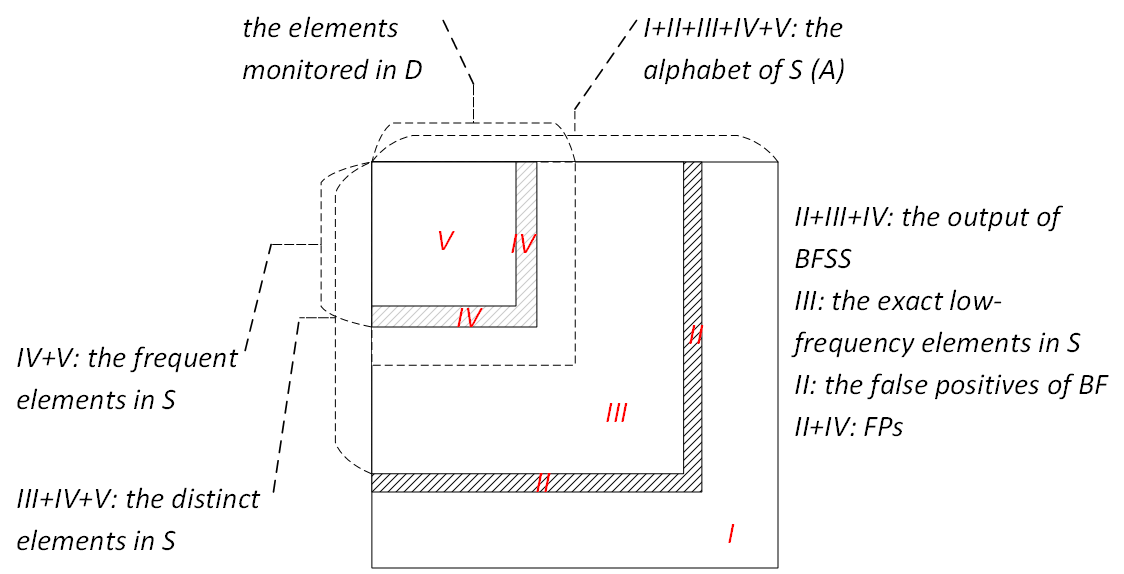
\includegraphics[width=3.5in]{png/bfss.png}
	\caption{The schematic diagram of the analysis of \emph{BFSS}}
	\label{fig:bfss}
\end{figure}

\subsubsection{\textbf{Analysis of FPs}}
In this section, we will give a theoretically bound of the expectation of the number of \emph{FPs} in the output of \emph{BFSS} regardless of the distribution of $S$, and a tighter bound can be derived for data streams under Pareto distribution \cite{IEEEexample:pareto}.

\begin{lemma}\label{lem:6}
Any item $e$ with $f_S(e)>\lfloor sN\rfloor+\lfloor\epsilon N\rfloor$ must not be output.
\end{lemma}

\begin{IEEEproof}
From Lemma \ref{lem:4}, we know that any item $e$ with $f_S(e)>\lfloor sN\rfloor+\lfloor\epsilon N\rfloor$ must be monitored in $D$, i.e. $e\in E$. Then from Lemma \ref{lem:5}, we can get that the items monitored in $D$ must satisfy $f_S(e)\leq f(e)$, and that is to say any item $e$ monitored in $D$ with $f_S(e)>\lfloor sN\rfloor+\lfloor\epsilon N\rfloor$ must satisfy $f(e)>\lfloor sN\rfloor+\lfloor\epsilon N\rfloor$. At last from Lemma \ref{lem:3}, we can prove that any item $e$ with $f(e)>\lfloor sN\rfloor+\lfloor\epsilon N\rfloor$ must satisfy $f(e)>\lfloor sN\rfloor+\Delta(e)$, which means $e$ will not be output.
\end{IEEEproof}

\begin{lemma}\label{lem:7}
The probability of a false positive of \emph{BF} is no more than:
\begin{equation}
(1-(1-\frac{1}{K})^{HM})^H
\end{equation}
\end{lemma}

\begin{IEEEproof}
A false positive of \emph{BF} means an item in $A$ not appearing in $S$ but not filtered out by \emph{BF}. Observe that after inserting $M$ keys into a table of size $K$, the probability that a particular bit is still 0 is exactly
\begin{equation} 
(1-\frac{1}{K})^{HM}
\end{equation}
\indent Hence the probability of a false positive in this situation is $(1-(1-\frac{1}{K})^{HM})^H$. However, we know that $M$ denotes the size of $A$ which is the alphabet of $S$, so the number of the distinct items in $S$ must be no more than $M$, i.e. $n\leq M$, and further we have $(1-(1-\frac{1}{K})^{Hn})^H\leq (1-(1-\frac{1}{K})^{HM})^H$.
\end{IEEEproof}

\begin{theorem}\label{thm:2}
Assuming no specific data distribution, the expectation of the number of \emph{FPs} in the output of \emph{BFSS}, denoted as $E(\#FPs)$, satisfies:
\begin{equation}\label{eq:7}
E(\#FPs)<M(1-(1-\frac{1}{K})^{HM})^H + \lfloor\frac{1}{s}\rfloor
\end{equation}
\end{theorem}

\begin{IEEEproof}
From Algorithm \ref{alg:bfss}, we can observe that two kinds of items contribute to \emph{FPs}: i) the false positives of \emph{BF}; ii) the items with $f_S(e)>\lfloor sN\rfloor$ wrongly output. The two cases correspond to the gray areas in Fig. \ref{fig:bfss} which is abstracted out from the analysis of \emph{BFSS}. Concretely speaking, the ligth gray area represents the items with $f_S(e)>\lfloor sN\rfloor$ wrongly output, i.e. the second case, and the dark gray area represents the items not filtered out by \emph{BF}, i.e. the first case. Furthermore, the output of \emph{BFSS} is represented by $II+III+IV$, and the exact low-frequency items in $S$ is represented by $III$.\par
For the first case, we define the independent 0-1 random variables $x_i(1\leq i\leq M)$ for each item in $A$, and the value of $x_i$ depends on whether $a_i$ appeared in $S$ or not. If $a_i$ appeared in $S$, then $x_i=0$; If not, then with a probability of $(1-(1-\frac{1}{K})^{Hn})^H$, $x_i=1$; From the defination of $x_i$, we can find that the expectation of the number of the false positives of \emph{BF} equals $E(\sum_{i=1}^{M}x_i)$, i.e. $(M-n)(1-(1-\frac{1}{K})^{Hn})^H$.\par 
For the second case, we know from Lemma \ref{lem:6} that items with $f_S(e)>\lfloor sN\rfloor+\lfloor \epsilon N\rfloor$ must not be not output, so only items with $\lfloor sN\rfloor<f_S(e)\leq \lfloor sN\rfloor+\lfloor \epsilon N\rfloor$ are likely to be output, and the maximum number of these items is $\lfloor\frac{1}{s}\rfloor$ because there are at most $\lfloor\frac{1}{s}\rfloor$ items with $f_S(e)>\lfloor sN\rfloor$ in $S$. From above, due to the linear properties of expectation, we can get:
\begin{equation}\label{eq:8}
E(\#FPs)\leq (M-n)(1-(1-\frac{1}{K})^{Hn})^H+\lfloor\frac{1}{s}\rfloor\\
\end{equation}
\indent In addition, $n\leq M$, so inequation \ref{eq:7} can be easily derived from inequation \ref{eq:8}.
\end{IEEEproof}
However, from above, we can see that $\frac{1}{s}$ is a very loose bound of the number of the items with $\lfloor sN\rfloor<f_S(e)\leq \lfloor sN\rfloor+\lfloor \epsilon N\rfloor$. We will get a tighter bound if $S$ .

\begin{theorem}\label{thm:3}
Assuming noiseless Pareto data with parameter $\alpha$ and $f_S(e_m)$, where $\alpha (>0)$ and $e_m$ denotes the item with the lowest frequency, we have:
\setlength{\arraycolsep}{0.0em}
\begin{eqnarray}
	E(\#FPs)<M(1-(1-\frac{1}{K})^{HM})^H + T\\
	T=min\{((\frac{f_S(e_m)}{\lfloor sN\rfloor})^\alpha-(\frac{f_S(e_m)}{\lfloor sN\rfloor+\lfloor \epsilon N\rfloor})^\alpha)M,\lfloor\frac{1}{s}\rfloor\}\label{eq:10}
\end{eqnarray}
\setlength{\arraycolsep}{5pt}
\end{theorem}

\begin{IEEEproof}
The Pareto distribution\footnote{https://en.wikipedia.org/wiki/Pareto\_distribution} has the following property: If $X$ is a random variable with a Pareto distribution, then the probability that $X$ is greater than some number $x$, i.e. the tail function, is given by:
$$Pr(X>x)=
\begin{cases}
(\frac{x_m}{x})^\alpha & x\geq x_m\\
1 & x<x_m
\end{cases}$$
where $x_m$ is the minimum possible value of $X$, and $\alpha$ is a positive parameter. In such case, the expected value of the number of the items with $\lfloor sN\rfloor<f_S(e)\leq \lfloor sN\rfloor+\lfloor \epsilon N\rfloor$ is $((\frac{f_S(e_m)}{\lfloor sN\rfloor})^\alpha-(\frac{f_S(e_m)}{\lfloor sN\rfloor+\lfloor \epsilon N\rfloor})^\alpha)n$.
\end{IEEEproof}
From Inequation \ref{eq:7}, we observe that the upper bound of $E(\#FPs)$ is related with the values of $H$ and $K$, in addtion, the value of $K$ directly influence the space consumption of \emph{BFSS}, and the value of $H$ directly influence the update time of \emph{BFSS}, so it is of great significance to choose the appropriate values of $K$ and $H$ to keep a good balance of the precision, the space consumption and the update time of \emph{BFSS} .


\subsubsection{\textbf{Space complexity}}\label{sec:space}
In this section, we will analyze the space complexity of \emph{BFSS} including how to choose the appropriate values of $H$ and $K$.

\textbf{Choosing the appropriate values of $H$ and $K$.}
Our goal is to choose the appropriate values of $H$ and $K$ to keep $\#FPs$ as small as possible, meanwhile, we have to take the space consumption and update time into consideration as well. However, we can only get the upper bound of the value of $E(\#FPs)$, which is not equivalent to $\#FPs$. In fact, from the Chernoff bound, we know that there is a high probability that an independent random variable hovers near its expected value, which means we can approximately treat $E(\#FPs)$ as $\#FPs$.\par
Obviously, the upper bound of $E(\#FPs)$ given in Inequation \ref{eq:7} is not so tight, and the upper bound of $E(\#FPs)$ given in Inequation \ref{eq:8} is much tighter. However, it is difficult for us to choose the appropriate values of $H$ and $K$ to minimize the upper bound given in Inequation \ref{eq:8} because the value of $n$ is variable, and the task will be much easier for the bound given in Inequation \ref{eq:7}, besides, the values of $M$ and $s$ are confirmed at the very beginning, therefore our task is to minimize the value of $(1-(1-\frac{1}{K})^{HM})^H$, denoted as $F$, and we have:
\begin{equation}\label{eq:11}
F\approx(1-e^{-\frac{HM}{K}})^H=e^{H\ln (1-e^{-\frac{HM}{K}})}
\end{equation}
Let $P=e^{-\frac{HM}{K}}$ and $G=H\ln (1-e^{-\frac{HM}{K}})$, and in order to minimize $F$, we only have to minimize $G$:
\begin{equation}\label{eq:12}
G=(-\frac{K}{M})\ln(P)\ln(1-P)
\end{equation}
The first derivative of $G$ with respect to $P$, denoted as $G'$, is:
\begin{equation}\label{eq:13}
G'=\frac{K}{M}(\frac{1}{1-P}\ln(P)-\frac{1}{P}\ln(1-P))
\end{equation}
From Equation \ref{eq:13}, we can easily observe that when $P=\frac{1}{2}$, $G$ reaches its minimum value. In this case, we have:
\begin{equation}\label{eq:14}
H=\frac{K}{M}\times\ln 2
\end{equation}
Combined with Equation \ref{eq:11} and Equation \ref{eq:14}, we have:
\begin{equation}\label{eq:15}
F\approx(1-e^{-\frac{HM}{K}})^H=(\frac{1}{2})^H\approx(0.6185)^{\frac{K}{M}}
\end{equation}
From the above derivation, we know that once the value of $\frac{K}{M}$ is confirmed, we can get the appropriate value of $H$ to minimize the value of $F$. For example, if the value of $\frac{K}{M}$ is set to 13, the appropriate value of $H$ is $\frac{K}{M}\times\ln 2\approx9.1$, because the value of $H$ is an integer, we set it to $\lfloor\frac{K}{M}\times\ln 2+\frac{1}{2}\rfloor=9$. Considering the length limit, we give a small fraction of the value of $F$ under various $\frac{K}{M}$ and $H$ combinations in Table \ref{tab:2}.\par
\begin{table} 
	\centering
	\caption{The value of $F$ under various $\frac{K}{M}$ and $H$ combinations.}
   \begin{tabular}{|c|c|c|c|c|c|c|}
   	\hline
   	$K/M$ & $H$& $H=8$ & $H=9$ & $H=10$ & $H=11$ & $H=12$\\ 
   	\hline
   	13&9.01&0.00199&0.00194&0.00198&0.0021&0.0023\\
   	\hline
   	14&9.7&0.00129&0.00121&0.0012&0.00124&0.00132\\
   	\hline
   	15&10.4&0.000852&0.000775&0.000744&0.000747&0.000778\\
   	\hline
   	16&11.1&0.000574&0.000505&0.00047&0.000459&0.000466\\
   	\hline
   	17&11.8&0.000394&0.000335&0.000302&0.000287&0.000284\\
   	\hline
   \end{tabular}
    	\label{tab:2}
\end{table}
For example, if $M=1M$ and $s=0.001$, then from Table \ref{tab:2}, we see that if $K=16M$, the value of $H$ should be $11$, therefore $F\approx0.000459$, and the upper bound of $E(\#FPs)$ ,calculated by Inequation \ref{eq:7}, is $1M\times0.000459+1/0.001=1459$. If $K=17M$, the corresponding values of $H$ and $F$ are 12 and 0.000284, therefore $E(\#FPs)=1284$. In fact, a much tighter bound of $E(\#FPs)$ can be derived from Inequation \ref{eq:8} once the value of $K$ and $H$ are confirmed.\par

\textbf{Analysis of $E(\#FPs)$.}
Our goal is to calculate the maximum possible value of $E(\#FPs)$ for different values of $n$ when the values of $H$ and $K$ are confirmed. Let $F(n)=(M-n)(1-(1-\frac{1}{K})^{Hn})^H$, and from Inequation \ref{eq:8}, we have $E(\#FPs)\leq F(n)+\lfloor\frac{1}{s}\rfloor$, in which the value of $\lfloor\frac{1}{s}\rfloor$ is confirmed once the value of $s$ is confirmed, therefore our task is to calculate the maximum value of $F(n)$. Let $t=(1-\frac{1}{K})^{H}(0<t<1)$, and we have:
\begin{equation}\label{eq:16}
F(n)=(M-n)(1-t^n)^H
\end{equation}
Obviously, when $0<n<M$, $F(n)>0$, and we have:
\begin{equation}
F(n)=e^{ln(M-n)+Hln(1-t^n)} \quad (0<n<M)
\end{equation}
Let $f(n)=ln(M-n)+Hln(1-t^n)$, therefore $F(n)=e^{f(n)}$, and our task is transformed to caculate the maximum value of $f(n)$. The first derivative of $f(n)$ with respect to $n$, denoted as $f'(n)$, is:
\begin{eqnarray}
f'(n)&=&\frac{1}{n-M}+\frac{Ht^nlnt}{t^n-1} \quad (0<n<M)\\
&=&\frac{1-t^{-n}+nHlnt-MHlnt}{(n-M)(1-t^{-n})}
\end{eqnarray}
Obviously, when $0<n<M$, $(n-M)(1-t^{-n})>0$. Let $g(n)=1-t^{-n}+nHlnt-MHlnt$, and the first derivative of $g(n)$ with respect to $n$, denoted as $g'(n)$, is:
\begin{equation}
g'(n)=t^{-n}lnt+Hlnt\quad (0<n<M)
\end{equation}
Obviously, $g'(n)<0$, which means the value of $g(n)$ decreases as the value of $n$ increases, therefore we can calculate the value of $n$ which makes the value of $f(n)$ maximum by solving the equation $g(n)=0$, and the value of $F(n)$ increases firstly and then decreases.
\begin{equation}
t^{-n}-1=nHlnt-MHlnt\quad (0<n<M)
\end{equation}
When $M=1M,K=16M$ and $H=11$, we have:
\begin{eqnarray}\label{eq:matlab}
(1-\frac{1}{16\times 10^6})^{-n}-1=11\times ln((1-\frac{1}{16\times 10^6}))n-\nonumber\\
10^6\times 11\times ln((1-\frac{1}{16\times 10^6})) (0<n<10^6)
\end{eqnarray}
The approximate integer solution of Equation \ref{eq:matlab}, solved by MATLAB, is 888640, and the corresponding value of $F(n)$ is 20, which means the maximum possible expected value of the false positives of \emph{BF} is 20 which is much smaller than the value calculated before, therefore $E(\#FPs)\leq 20+1/0.001=1020$ when $s=0.1\%$. Fig. \ref{fig:F(n)-16000000} shows the value of $F(n)$ when $M=1M,K=16M$ and $H=11$ from which we can observe that the value of $F(n)$ increases firstly and decreases at last just as we have theoretically proved before, and when $n<400000$, the value of $F(n)$ is nearly 0. Fig. \ref{fig:n-F(n)} shows the maximum value of $F(n)$ and the corresponding value of $n$ when $M=1M$ varying the the value of $\frac{K}{M}$, and we set $H=\lfloor \frac{K}{M}\times ln2+\frac{1}{2}\rfloor$ as discussed before. Fig .\ref{subfig:n} shows that the value of $n$ increases as the value of $\frac{K}{M}$ increases. From Fig. \ref{subfig:F(n)}, we observe that the value of $F(n)$ decreases rapidly as the value of $\frac{K}{M}$ increases, however, the larger the values of $K$ and $H$ are, the more space and update time \emph{BFSS} will consume. Taking the number of \emph{FPs}, update time and space available into consideration, we can choose the appropriate values of $K$ and $H$.

\begin{figure}
	\centering
	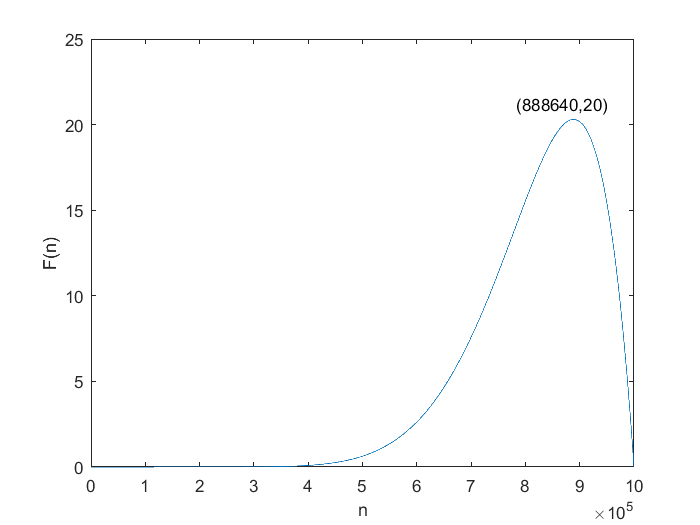
\includegraphics[width=3in]{png/F(n)-16000000.png}
	\caption{The value of $F(n)$ when $M=1M,K=16M$ and $H=11$}
	\label{fig:F(n)-16000000}
\end{figure}

\begin{figure}[!t]
	\centering
	\begin{minipage}{0.47\linewidth}
		\centering
		\subfloat[]{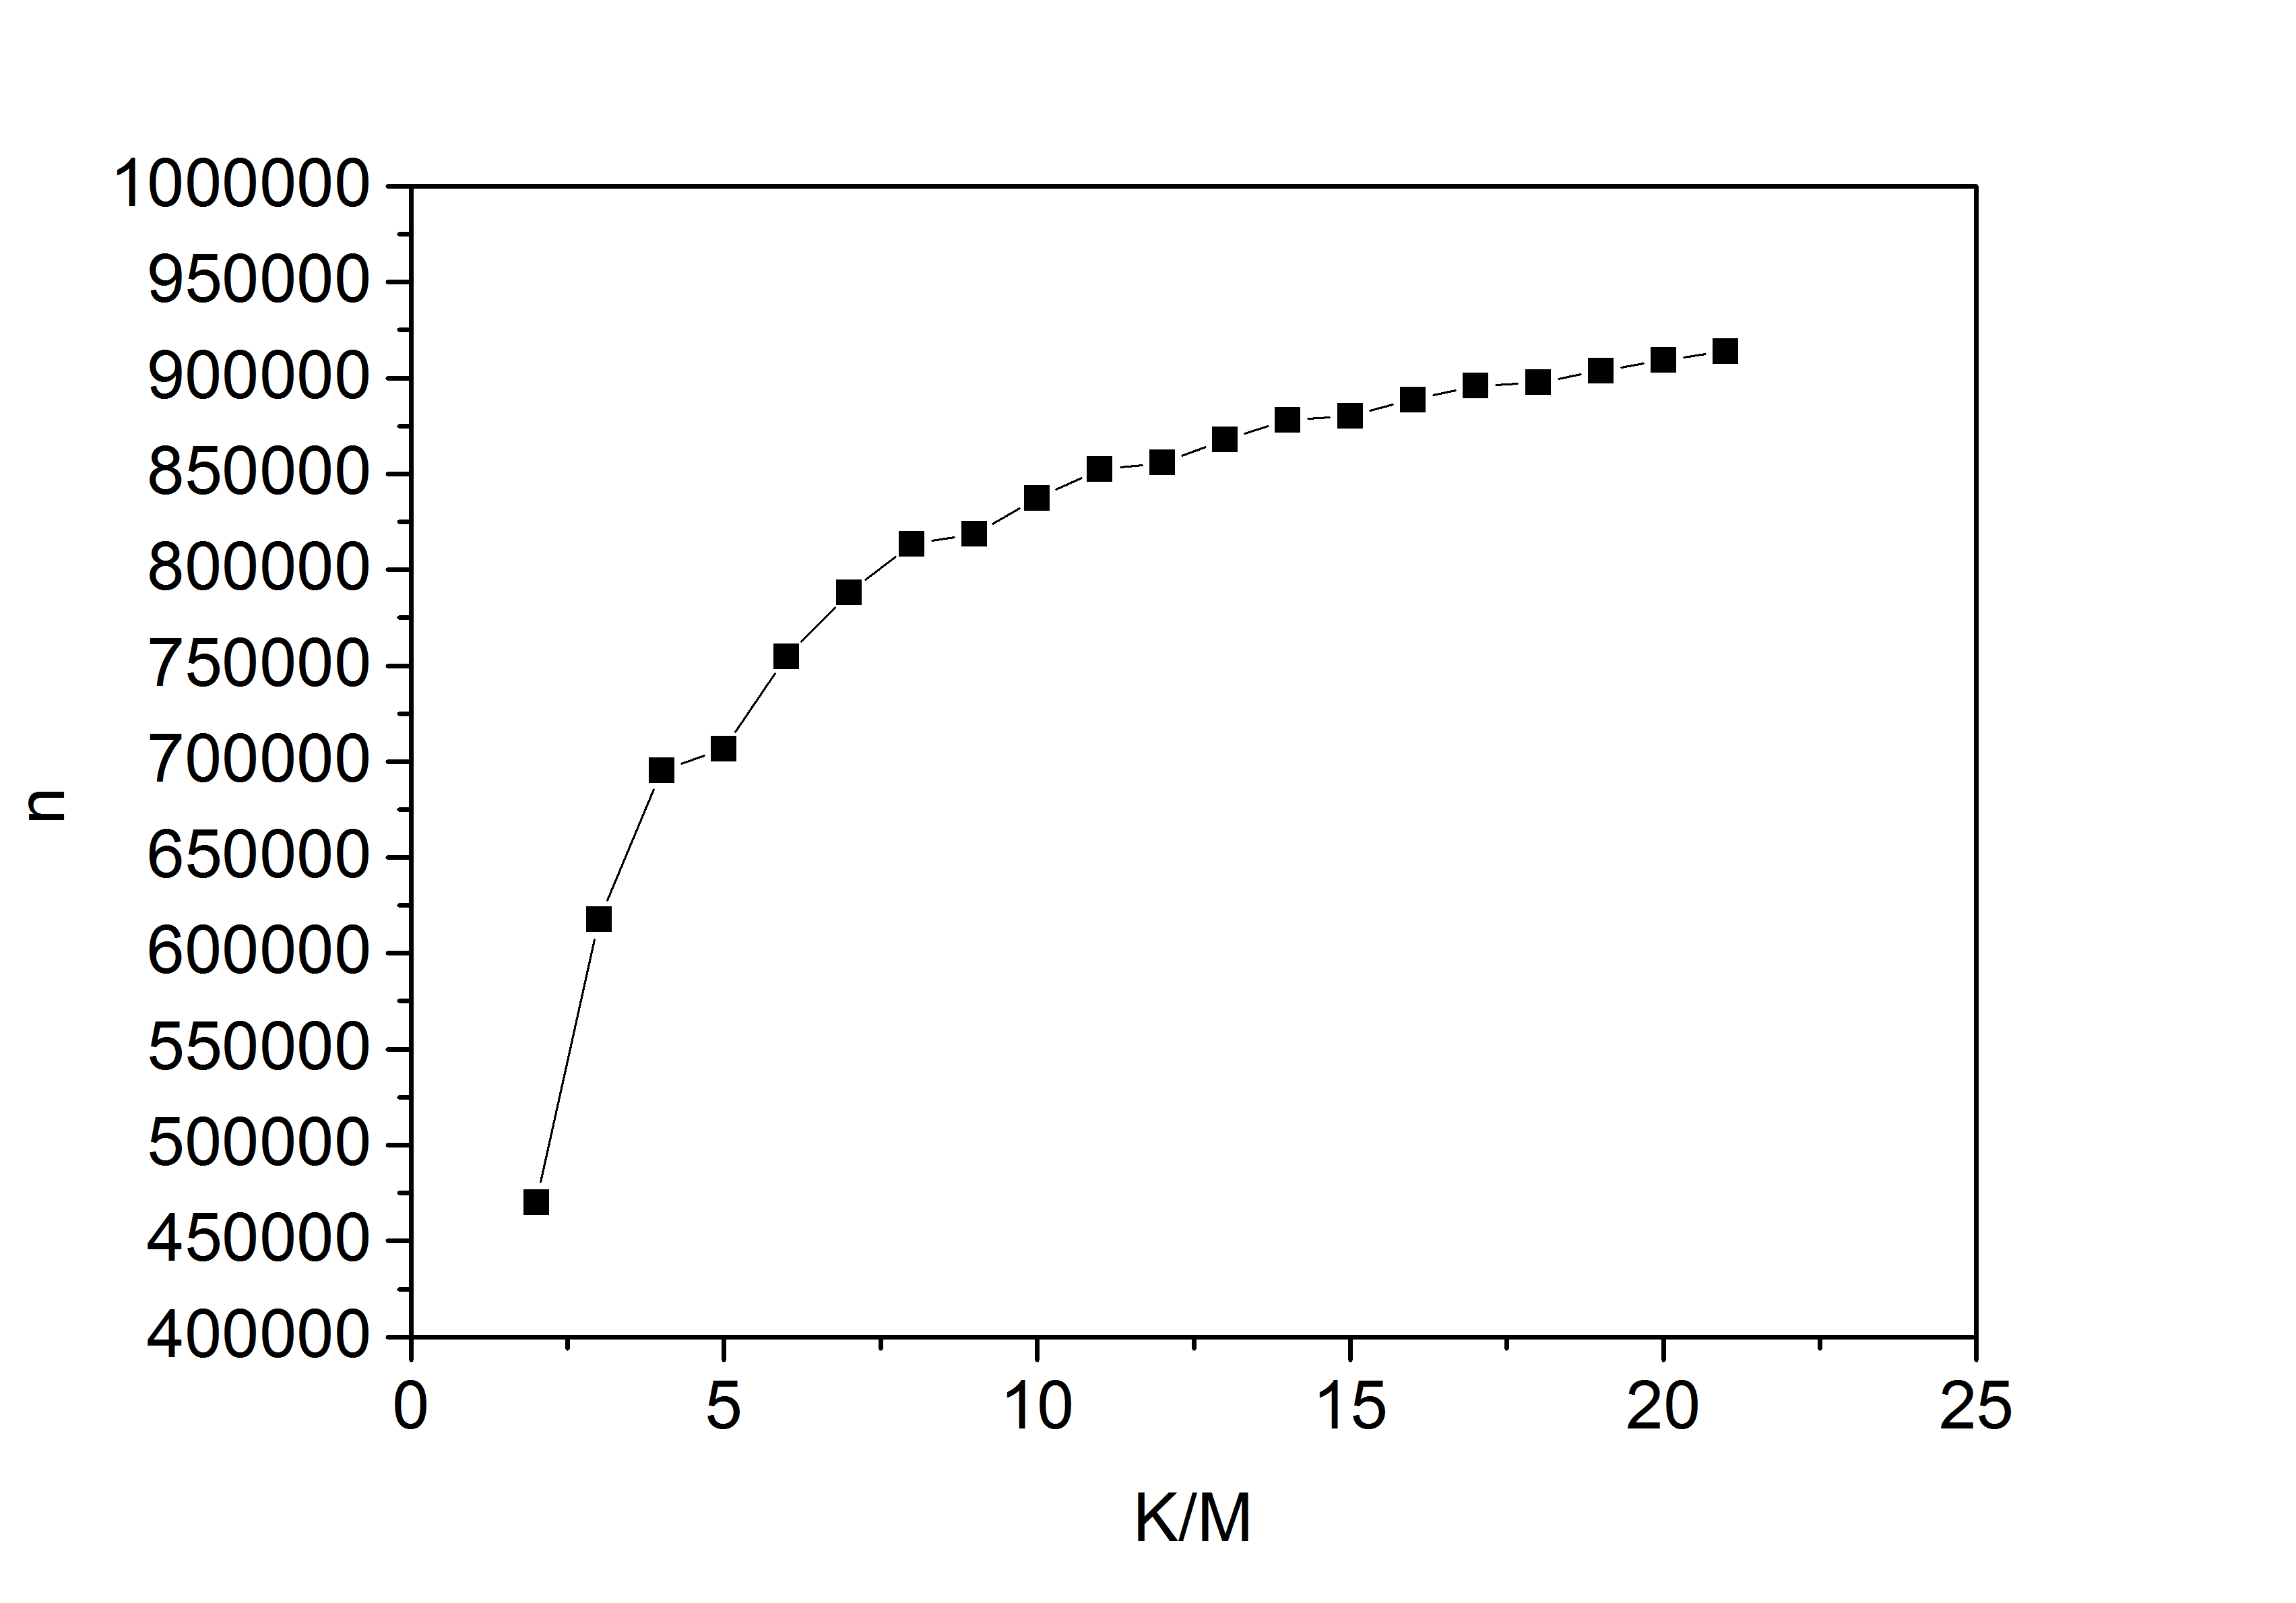
\includegraphics[width=1.9in]{png/n.png}\label{subfig:n}}
	\end{minipage}
	\begin{minipage}{0.47\linewidth}
		\centering
		\subfloat[]{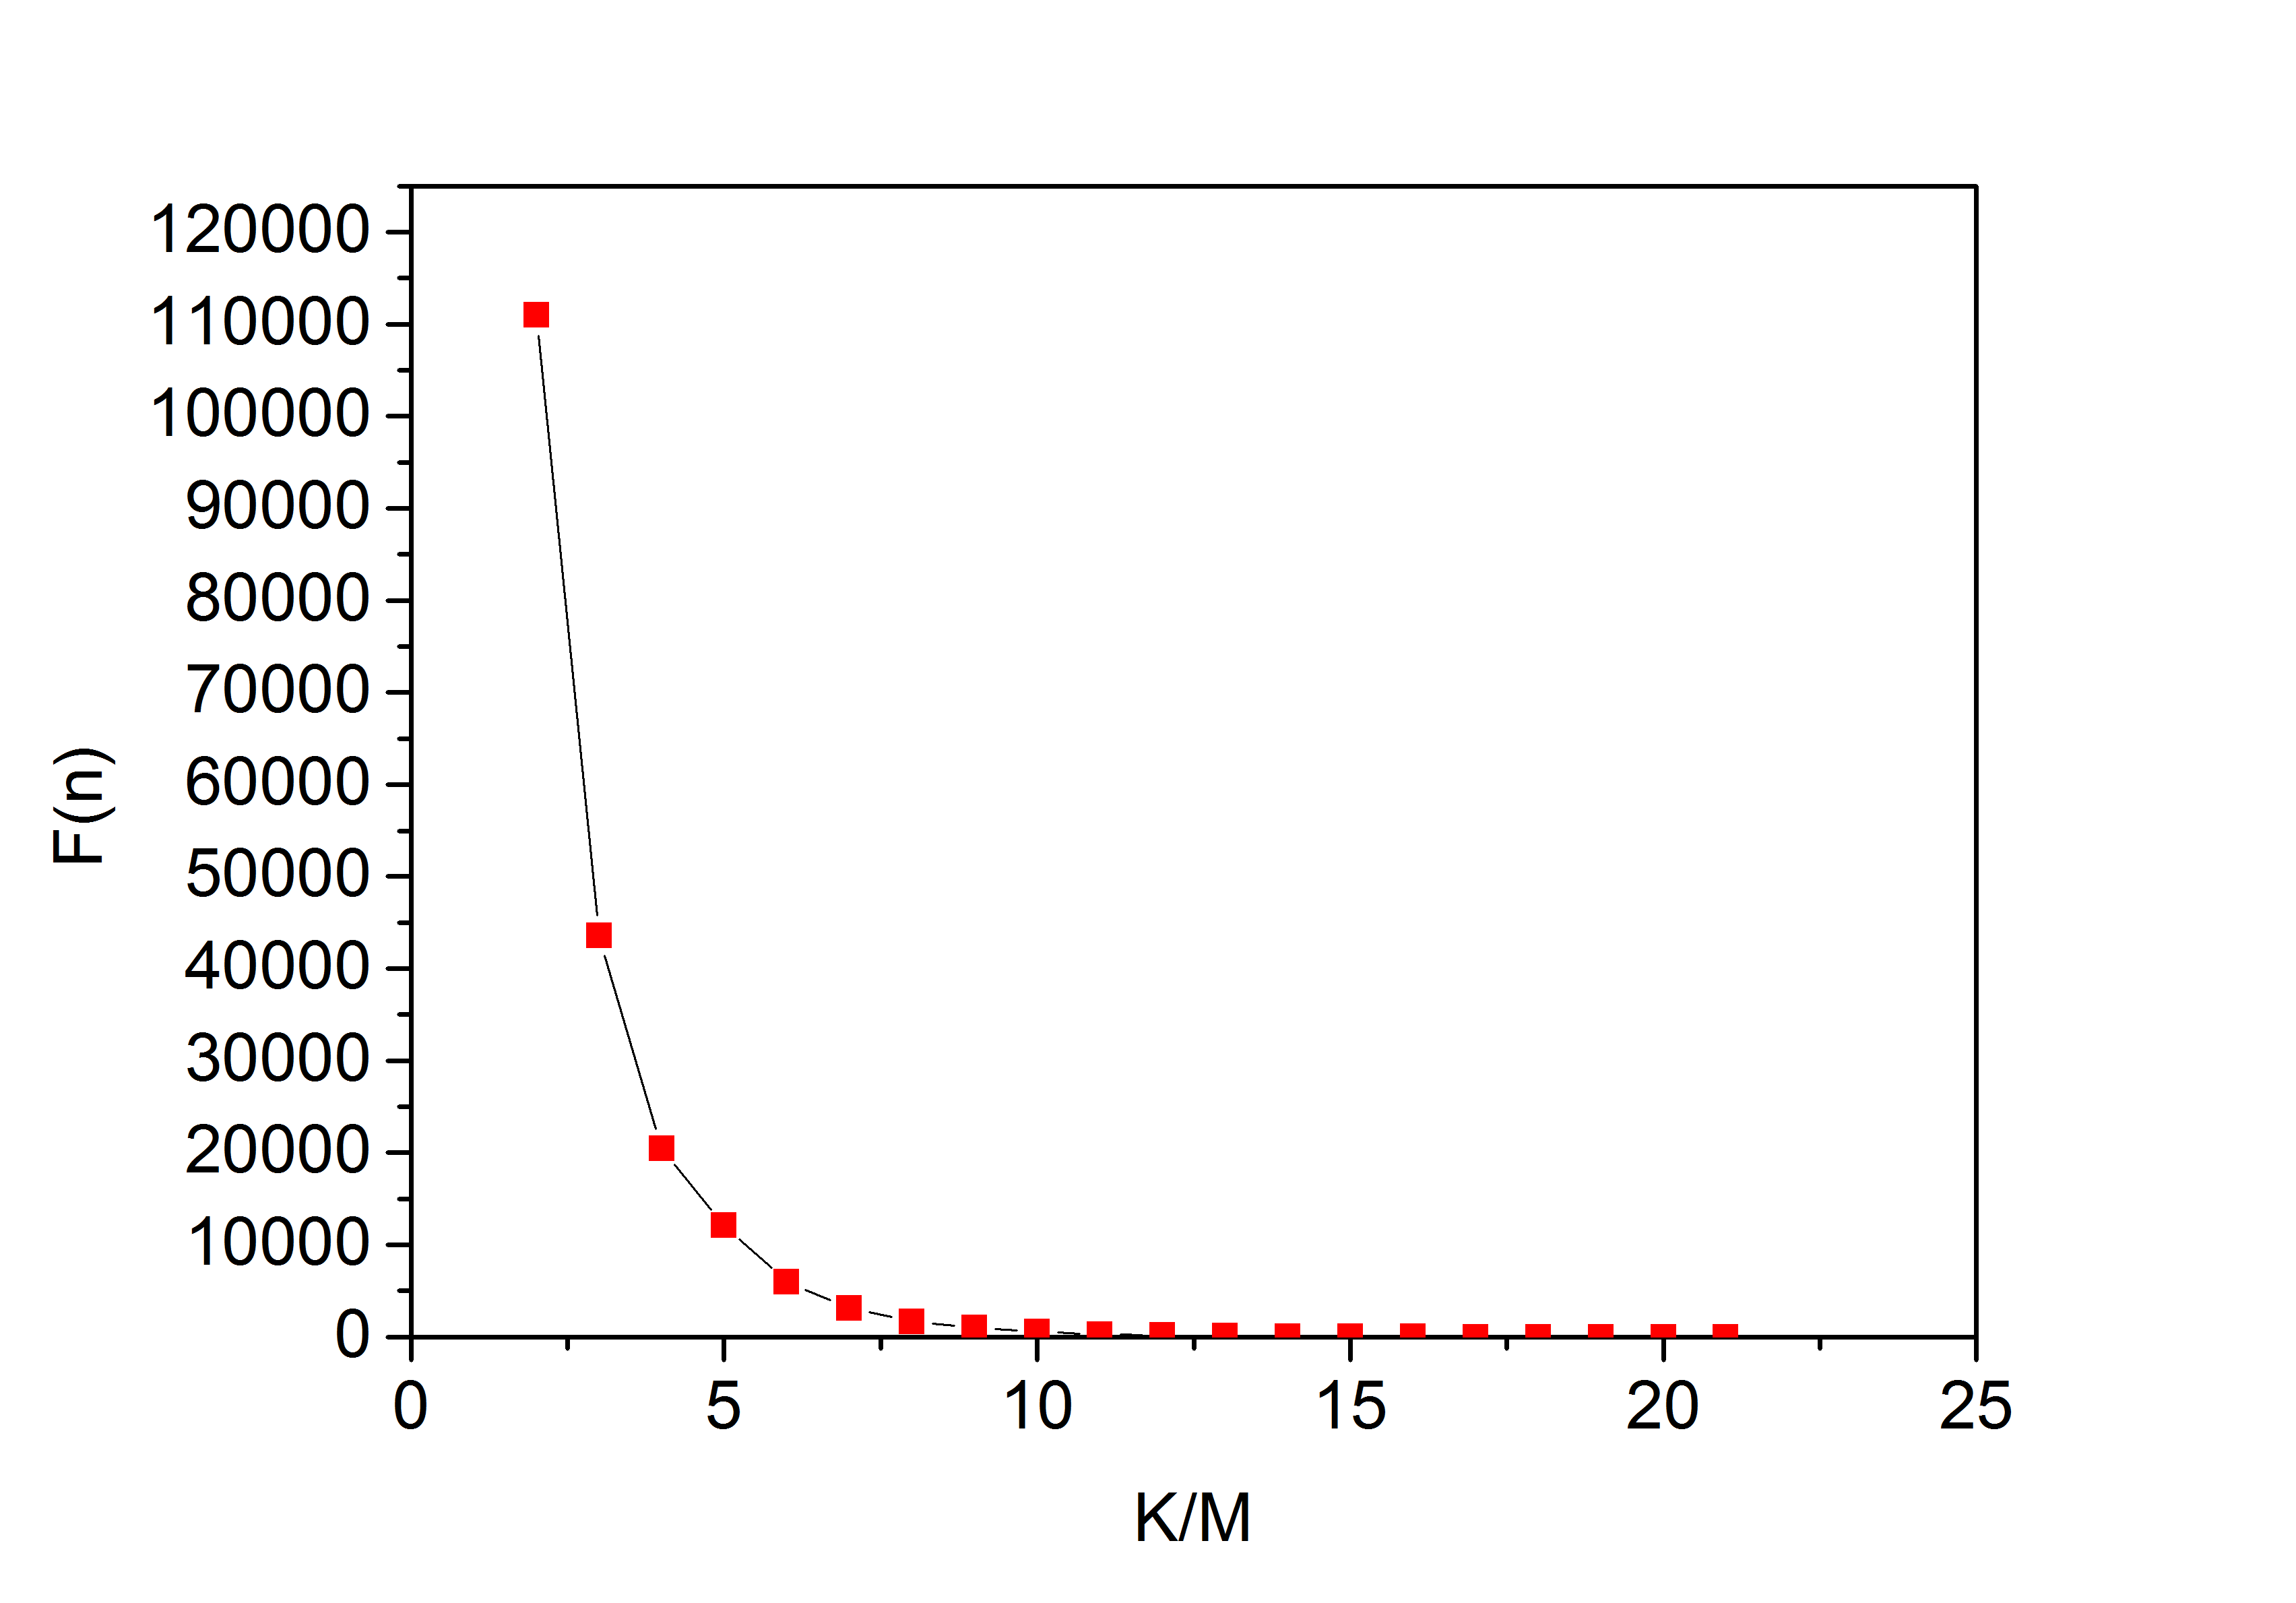
\includegraphics[width=1.9in]{png/F(n).png}\label{subfig:F(n)}}
	\end{minipage}
	\caption{The maximum value of $F(n)$ and the corresponding value of $n$ when $M=1M$ - Varying $\frac{K}{M}$.}
	\label{fig:n-F(n)}
\end{figure}

\begin{theorem}\label{thm:4}
The space complexity of \emph{BFSS} is $O(\lambda M+ min(\lceil\frac{1}{\epsilon}\rceil,M))$, where $\lambda\in N^*$, the value of which has been discussed above. 
\end{theorem}
\begin{IEEEproof}
The space complexity of \emph{BFSS} includes two part: i) the size of \emph{BF}, i.e. $K$. ii) the number of counters used in $D$, i.e. $m$. In order to get the minimum value of $E(\#FPs)$, the value of $K$ should be multiple times of the value of $M$, i.e. $K=\lambda M(\lambda\in N^*)$. From Algorithm \ref{alg:output}, we have $m\leq min(\lceil\frac{1}{\epsilon}\rceil,M)$. So the space complexity of \emph{BFSS} is $O(\lambda M+ min(\lceil\frac{1}{\epsilon}\rceil,M))$.
\end{IEEEproof}
In conclusion, there exists a trade off between the number of \emph{FPs} and the space consumption of \emph{BFSS}. Theoretically, once $M$ is confirmed, the larger the value of $\lambda$ is, the larger the value of $K$ will be, and the smaller the value of $E(\#FPs)$ will be.\par
Furthermore, consider a naive method to solve $s$\emph{-BLFE}: we simply allocate each item in $A$ a counter, and update the corresponding counter for each item in $S$, when a query comes, we just output the items with $f_S(e)\leq\lfloor sN\rfloor$. Obviously the method can maintain the low-frequency items precisely, and the space complexity of the method is $O(M)$. \emph{BFSS} has no advantage over the naive method in space complexity considering big O though, \emph{BFSS} needs not to store the exact value or the fingerprint of each item which may consume much space especially when the value is long string, like URL. The experimental results indicate \emph{BFSS} is much more space efficient.
\subsubsection{\textbf{Time complexity}}
In this section, we will discuss the time complexity of \emph{BFSS}.

\begin{theorem}\label{thm:5}
Processing each item needs $O(1)$ time, independent of $N$.
\end{theorem}

\begin{IEEEproof}
From Algorithm \ref{alg:bfss}, we know the processing time for each item has two parts: i) the time spent hasing each item into \emph{BF}. ii) the time spent updating the corresponding counter in $D$. Obviously, the time spent hashing each item into \emph{BF} is constant because $H$ is constant. Consider two cases in updating the corresponding counter in $D$: i) item $e$ is monitored in $D$, and we only have to update the corresponding counter. ii) item $e$ is not monitored in $D$, and we have to locate the counter with the minimum $f(e)$ first, then update it. Obviously, the time spent for any case is constant because $\lceil \frac{1}{\epsilon}\rceil$ is constant. Therefore, processing each item needs $O(1)$ time.
\end{IEEEproof}

\subsubsection{\textbf{Challenges to BFSS}}
In this section, we will identify the existing problems in \emph{BFSS}.\par
From the analysis in section \ref{sec:space}, we observe that $K$ should increase monotonically with $M$ in order to keep a low rate of \emph{FPs}, however, what if the space available is limited and small? The precision of \emph{BFSS} will be very low in this case.\par
Inspired by the algorithm proposed in \cite{IEEEexample:sbf}, we present the \emph{SBFSS} algorithm, which can find low-frequency items over data streams in limited and small space with a few \emph{FPs} together with theoretically bounded number of \emph{FNs}.\par

\subsection{The BFSS* Algorithm}
In this section, we will introduce \emph{BFSS*}, which approximately estimates the distribution of a data stream.\par
The goal of \emph{BFSS*} is to estimate the percentage of the number of the items whose frequency is above a user-specified support, denoted as $p_1$, and the percentage of the total frequencies of these items, denoted as $p_2$.\par 
\emph{BFSS*} and \emph{BFSS} share the same update process, and the query process of \emph{BFSS*} is described in Algorithm \ref{alg:bfss*}. For each item $e$ in $A$, we first check whether it is in \emph{BF}, if the item is in \emph{BF}, we increment the counter $n$, and if the item appears in $D$ and $f(e)>\lfloor sN\rfloor+\Delta(A[i])$, we increment $n'$ and add $f(e)-\Delta(e)$ to $f$. At last, we set $p_1'=n_s'/n'$ as the approximate value of $p_1$ and $p_2'=f'/N$ as the approximate value of $p_2$.

\begin{algorithm}[h]
	\caption{BFSS* Query Algorithm}
	\label{alg:bfss*}
	\begin{algorithmic}[1]
		\REQUIRE \emph{BF}, $D$, $s$, $A$, $N$, $M$
		\ENSURE The percentage of the items whose frequency is above $\lfloor s
		N\rfloor$ and the percentage of the total frequencies of these items
	    \STATE $flag=true,n_s'=0,n'=0,f_s'=0,p_1'=0,p_2'=0$;\COMMENT{\emph{flag}: indicate whether an item is in \emph{BF}, $n$: the number of distinct items in $S$, $n_s'$: the estimated number of the items whose frequency is above $\lfloor sN\rfloor$, $f_s'$: the estimated total frequencies of the items whose frequency is above $\lfloor sN\rfloor$, $p_1'$: the estimated percentage of the items whose frequency is above $\lfloor sN\rfloor$, $p_2'$: the estimated percentage of the total frequencies of these items.}
	    \FOR{$i=0$ to $M-1$}
    	\STATE $flag=true;$
    	\FOR{$j=1$ to $H$}
	    \IF{$BF[h_j(A[i])]==0$}
	    \STATE $flag=false;$
	    \STATE break;
	    \ENDIF
	    \ENDFOR
	    \IF{$flag==true$}
	    \STATE $n'=n'+1;$
	    \IF{$A[i]$ is monitored in $D$}
	    \IF{$f(A[i])> \lfloor s N\rfloor+\Delta(A[i])$}
	    \STATE $n_s'=n_s'+1;$
	    \STATE $f_s'=f_s'+(f(A[i])-\Delta(A[i]));$
	    \ENDIF
	    \ENDIF
	    \ENDIF
	    \ENDFOR
	    \STATE $p_1'=n_s'/n',p_2'=f_s'/N;$
	    \STATE Output $p_1',p_2';$
	\end{algorithmic}
\end{algorithm}

\subsection{Analysis of BFSS*}
In this section, we will give theoretical analysis of $p_1$ and $p_2$. Obviously, the time and space complexity of \emph{BFSS*} are the same as \emph{BFSS}, and we don't discuss here.
\subsubsection{\textbf{Analysis of $p_1$}}
From the defination of $p_1$, we know that $p_1=\frac{n_s}{n}$, in which $n_s$ denotes the exact number of the items whose frequency is above $s$. From Lemma \ref{lem:3} and Lemma \ref{lem:5}, we observe two facts: i) any item with $f_s(e)>\lfloor sN\rfloor+\lfloor \epsilon N\rfloor$ must satisfy $f(e)>\lfloor sN\rfloor+\Delta(e)$. ii) any item with $f_s(e)\leq\lfloor sN\rfloor$ must satisfy $f(e)\leq\lfloor sN\rfloor+\Delta(e)$. From the two facts, we know that only items with $\lfloor sN\rfloor<f_s(e)\leq \lfloor sN\rfloor+\lfloor \epsilon N\rfloor$ are likely to be neglected, which means $n_s\geq n_s'$. Let $\Delta(n_s)=n_s-n_s'$, and the maximum value of $\Delta(n_s)$  is the number of the items with $\lfloor sN\rfloor<f_s(e)\leq \lfloor sN\rfloor+\lfloor \epsilon N\rfloor$. Obviously, for any data stream, $\Delta(n_s)\leq\lfloor\frac{1}{s}\rfloor$, which is a very loose bound, and for data streams under Pareto distributions, we have $E(\Delta(n_s))\leq((\frac{f_S(e_m)}{\lfloor sN\rfloor})^\alpha-(\frac{f_S(e_m)}{\lfloor sN\rfloor+\lfloor \epsilon N\rfloor})^\alpha)n$, the proof of which can be found in the proof of Theorem \ref{thm:3}.\par
From Algorithm \ref{alg:bfss*}, we can get $n'\geq n$ because \emph{BF} causes no false negatives but only false positives. Let $\Delta(n)=n'-n$, and the value of $\Delta(n)$ equals to the number of the false positives caused by \emph{BF}. Therefore, we have $E(\Delta(n))=(M-n)(1-(1-\frac{1}{K})^{Hn})^H<M(1-(1-\frac{1}{K})^{HM})^H$, the proof of which can be found in the proof of Theorem \ref{thm:2}.\par
From above, $p_1'=\frac{n_s-\Delta(n_s)}{n+\Delta(n)}\leq p_1$, and we can theoretically get the upper bound of $E(\Delta(n_s))$ for data streams under Pareto distributions and the upper bound of $E(\Delta(n))$ for any data streams. Furthermore, we can minimum $E(\Delta(n))$ by selecting appropriate parameters, which has been discussed before. Experimental results in \cite{IEEEexample:overview,IEEEexample:overview_vldbj} show that \emph{Space Saving} has a very high precision (almost 1), which means the number of the items with $\lfloor sN\rfloor-\lfloor \epsilon N\rfloor<f_s(e)\leq\lfloor sN\rfloor$ wrongly output is very small, and if we set $s=s+\epsilon$, then the number of the items with $\lfloor sN\rfloor<f_s(e)\leq\lfloor sN\rfloor+\lfloor \epsilon N\rfloor$ wrongly output is vary small too, in other words, the value of $\Delta(n_s)$ is very small. In fact, the experimental results also show that $p_1'$ is nearly the same as $p_1$.
\subsubsection{\textbf{Analysis of $p_2$}}
From the defination of $p_2$, we can get $p_2=\frac{f_s}{N}$, in which $f_s$ denotes the exact total frequencies of the items whose frequency is above $\lfloor sN\rfloor$. Obviously, $f_s\geq f_s'$ because we may neglect some items with $\lfloor sN\rfloor<f_s(e)\leq\lfloor sN\rfloor+\lfloor \epsilon N\rfloor$ just like the analysis of $p_1$, besides, for the items with $f(e)>\lfloor sN\rfloor+\Delta(e)$, we just add $(f(e)-\Delta(e))(\leq f_s(e))$ to $f_s'$. Let $\Delta(f_s)=f_s-f_s'$, from above, $\Delta(f_s)$ consists of two parts: i) the total frequencies of the items with $\lfloor sN\rfloor<f_s(e)\leq\lfloor sN\rfloor+\lfloor \epsilon N\rfloor$ wrongly neglected, denoted as $\Delta_1(f_s)$. ii) the total missing frequencies of the items with $f(e)>\lfloor sN\rfloor+\Delta(e)$, denoted as $\Delta_2(f_s)$. For $\Delta_1(f_s)$, obviously, we have $\Delta_1(f_s)\leq\Delta(n_s)\times(\lfloor sN\rfloor+\lfloor \epsilon N\rfloor)$, in which $\Delta(n_s)$, for \emph{Space Saving}, is very small (nearly 0). For $\Delta_2(f_s)$, we have $\Delta_2(f_s)\leq\lceil\frac{1}{s}\rceil\times\lfloor\epsilon N\rfloor$ because there are at most $\lceil\frac{1}{s}\rceil$ items with $f(e)>\lfloor sN\rfloor+\Delta(e)$, then from Lemma \ref{lem:5} and Lemma \ref{lem:3}, we have $f_s(e)-(f(e)-\Delta(e))\leq\Delta(e)\leq\lfloor\epsilon N\rfloor$.\par
From above, $p_2'=\frac{f_s-(\Delta_1(f_s)+\Delta_2(f_s))}{N}\leq p_2$. Let $\Delta(p_2)=p_2-p_2'$, and we have $\Delta(p_2)\leq\frac{\Delta(n_s)\times(\lfloor sN\rfloor+\lfloor \epsilon N\rfloor)+\lceil\frac{1}{s}\rceil\times\lfloor\epsilon N\rfloor}{N}$. In fact, the experimental results show that $p_2'$ is a little smaller than $p_2$.

\subsection{The SBFSS Algorithm}\label{sec:sbfss}
In this section, we will introduce \emph{SBFSS}, which modifies \emph{BFSS} and can find low-frequency items in data streams using limited and small space.\par
The major difference between \emph{BFSS} and \emph{SBFSS} is the Bloom filter we use. Concretely speaking, \emph{BF} is a regular Bloom filter, while \emph{SBF} change bits in \emph{BF} into cells, each consisting of one or more bits. In addition, from the explaination above, the size of \emph{BF}, i.e. $K$, should increase monotonically with $M$, however, there can be no linear relationship between the size of \emph{SBF}, i.e. $K'$, and $M$, and $K'$ can be any integer predefined by users. Defination \ref{def:1} is the detailed defination of \emph{SBF}.\par  

\newtheorem{defn}{Definition}
\begin{defn}\label{def:1}
\emph{SBF} is defined as an array of integer $SBF[1],SBF[2],...,SBF[k]$ whose minimum value is 0 and maximum value is $max$. Each item of the array is allocated $d$ bits. The relation between $max$ and $d$ is then $max=2^d-1$. Compared to bits in a regular Bloom filter, each item of the \emph{SBF} is called a cell.
\end{defn}

Like \emph{BFSS}, \emph{SBFSS} consists of two phases: updating and quering. Algorithm \ref{alg:sbfss} and Algorithm \ref{alg:soutput} give the detailed descriptions of them. Due to the length limit, no more tautology here.


\begin{algorithm}[h]
	\caption{SBFSS Update Algorithm}
	\label{alg:sbfss}
	\begin{algorithmic}[1]
		\REQUIRE Stream $S$, support threshold $s$
		\STATE The form of the counters in $D$ is $(e,f(e),\Delta(e))$
		\FOR{$i=0$ to $k-1$}
		\STATE $SBF[i]=0$
		\ENDFOR
		\FOR{each item $e$ of stream $S$}
		\STATE Select $P$ different cells uniformly at random $SBF[j_1]...SBF[j_P]$, $P\in \{1,...,k\}$
		\FOR{each cell $SBF[j]\in\{SBF[j_1]...SBF[j_P]\}$}
		\IF{$SBF[j]\geq 1$}
		\STATE $SBF[j]=SBF[j]-1$
		\ENDIF
		\ENDFOR
	    \FOR{$i=1$ to $H$}
		\STATE $SBF[h_i(e)]=max$
		\ENDFOR
		\IF{$e$ is monitored in $D$}
		\STATE $f(e)=f(e)+1$;
		\ELSIF{$m<C$}
		\STATE Assign a new counter $(e,1,0)$ to it
		\STATE $m=m+1$
		\ELSE
		\STATE Let $e_m$ be the item with least hits, $min$
		\STATE Replace $e_m$ with $e$ in $D$
		\STATE $f(e)=min+1,\Delta(e)=min$
		\ENDIF
		\STATE $N=N+1$;
		\ENDFOR
	\end{algorithmic}
\end{algorithm}

\begin{algorithm}[h]
	\caption{SBFSS Query Algorithm}
	\label{alg:soutput}
	\begin{algorithmic}[1]
		\REQUIRE \emph{SBF}, $D$, $s$, $A$, $N$, $M$
		\ENSURE low-frequency items with threshold $s$
		\STATE $flag=true$; \COMMENT{ \emph{flag}: indicate whether an item is in \emph{SBF} or not}
		\FOR{$i=0$ to $M-1$}
		\STATE $flag=true$
		\FOR{$j=1$ to $H$}
		\IF{$SBF[h_j(A[i])]==0$}
		\STATE $flag=false$
		\STATE break;
		\ENDIF
		\ENDFOR
		\IF{$flag==true$}
		\IF{$A[i]$ is monitored in $D$}
		\IF{$f(A[i])\leq\lfloor sN\rfloor+\Delta(A[i])$}
		\STATE output $A[i]$ as a low-frequency item
		\ENDIF
		\ELSE
		\STATE output $A[i]$ as a low-frequency item
		\ENDIF
		\ENDIF
		\ENDFOR
	\end{algorithmic}
\end{algorithm}

From Algorithm \ref{alg:sbfss}, we observe that there are two kinds of operation on \emph{SBF}. First randomly decrement $P$ cells by 1 so as to make room for fresh items; then set the same $H$ cells as in the update process to $max$.\par 
Intuitively, due to the random deletion operation, \emph{SBF} does not exceed its capacity in a data stream scenario, however, false negatives may come up as well.

\subsection{Analysis of SBFSS}
Like \emph{BFSS}, we will give theoretical analysis of \emph{SBFSS} in this section, including the equivalence of \emph{SBF'} (the \emph{SBF} used in \cite{IEEEexample:sbf}) and \emph{SBF}, \emph{FNs}, \emph{FPs}, parameters setting, and time complexity.\par
\subsubsection{\textbf{Analysis of the equivalence of SBF' and SBF}}
\emph{SBF'} is used to detect duplicates over data streams, in fact, from Algorithm \ref{alg:sbfss} and Algorithm \ref{alg:soutput}, we can observe that \emph{SBF} is used to filter out the items that never appeared in $S$, and we check whether the item in $A$ is duplicated one by one, if the item is a duplicate, we just claim it appeared in $S$, in this sense, \emph{SBF'} and \emph{SBF} share the same function. So the properties of \emph{SBF'}, including the probability of a false positive and a false negative of \emph{SBF'}, are fully applicable to \emph{SBF}.\par

\subsubsection{\textbf{Analysis of FPs}}
In this section, we will give a theoretically upper bound of the expectation of the number of \emph{FPs} in the ouput of \emph{SBFSS}.\par
The detailed proof of Lemma \ref{lem:8} can be found in \cite{IEEEexample:sbf}. Because of the limitation of length, no more tautology here.
\begin{lemma}\label{lem:8}
The probability of a false positive (FP) of \emph{SBF} is no greater than :
\begin{equation}
(1-(\frac{1}{1+\frac{1}{P(1/H-1/m)}})^{max})^H
\end{equation}
\end{lemma}

\begin{theorem}\label{thm:6}
Assuming no specific data distribution, the expectation of the number of \emph{FPs} in the output of \emph{SBFSS}, denoted as $E'(\#FPs)$, satisfies:
\begin{eqnarray}\label{eq:17}
E'(\#FPs)<M \min \{(1-(\frac{1}{1+\frac{1}{P(1/H-1/m)}})^{max})^H,\\\nonumber
	(1-(1-\frac{1}{k})^{HM})^H\} + \lceil\frac{1}{s}\rceil
\end{eqnarray}
\end{theorem}

\begin{IEEEproof}
From Fig. \ref{fig:sbfss}, we notice that the \emph{FPs} of \emph{SBFSS} has two parts: i) the false positives of \emph{SBF}, i.e. $II$; ii) the items with $f_S(e)>\lfloor sN\rfloor$ wrongly output, i.e. $VI$. In fact, $V$ is the only difference between the \emph{FPs} of \emph{SBFSS} and the \emph{FPs} of \emph{BFSS}, for \emph{BFSS}, the items in $V$ will be output, however, due to the false negatives of \emph{SBF} in \emph{SBFSS}, i.e. $IV+V+VIII$, the items in $V$ will be neglected by \emph{SBFSS}, in this sense, the false negatives of \emph{SBF} inversely reduce the number of \emph{FPs} of \emph{SBFSS}. \par
In fact, the posibility of a false positive of \emph{SBF} must be smaller than that of \emph{BF} under the same conditions because \emph{SBF} brings in decrement operation. For the first case, we can get the upper bound of the expectation of the number of the false positives of \emph{SBF} through Lemma \ref{lem:7} and Lemma \ref{lem:8}. For the second case, it is clearly to see from Fig. \ref{fig:sbfss} that the maximum of the area of $VI$ is $\lceil\frac{1}{s}\rceil$, which is the area of the square surrounded by dotted lines, and obviously it is a loose bound. The residual derivation is obvious and exactly the same as Theorem \ref{thm:2}, and no more tautology here.
\end{IEEEproof}
Like \emph{BFSS}, a tighter bound of the area of $VI$ can be obtained if we assume the distribution of $S$, and the bound is $(\frac{f_S(e_m)}{\lfloor sN\rfloor})^\alpha(1-\frac{1}{2^\alpha})M$, the derivation of which is exactly the same as E.q. \ref{eq:10}, if the distribution is Pareto. In addition, due to the exsitence of $V$, the number of the elemens with $f_S(e)>\lfloor sN\rfloor$ wrongly output is smaller than that of \emph{BFSS} regardless of the data distribution of $S$. 
\begin{figure}
	\centering
	\includegraphics[width=3.5in]{png/sbfss.png}
	\caption{The schematic diagram of the analysis of \emph{SBFSS}}
	\label{fig:sbfss}
\end{figure}

\subsubsection{\textbf{Analysis of FNs}}
In this section, unlike \emph{BFSS}, we will give a theoretically upper bound of the expectation of the number of \emph{FNs} in the ouput of \emph{SBFSS}. \par
From Fig. \ref{alg:sbfss}, we can see that the \emph{FNs} of \emph{SBFSS}, $IV$, is a portion of the false negatives of \emph{SBF}, $IV+V+VIII$. Therefore the upper bound of the number of \emph{FNs} in the output of \emph{SBFSS} is the number of the false negatives of \emph{SBF}.\par
First, let us consider the probability of a false negative of \emph{SBF} which is an error when an item in $S$ wrongly filtered out by \emph{SBF}. Therefore only the items in $S$ can generate false negatives, obviously the number of false negatives is related to the input data distribution.\par
Suppose an item $A[i]$ appearing in $S$ whose last appearence in $S$ before a query comes is $e_{i-\delta_i}$, where $\delta_i$ represents the number of items in $S$ during the time between the last appearance of $A[i]$ and a query, is hashed into $H$ cells, $SBF[C_{i1}],...,SBF[C_{iH}]$. A false negative happens if any of those $H$ cells is decremented to 0 during the $\delta_i$ iterations when a query comes. Let $PR_0(\delta_i,p'_{ij})$ be the probability that cell $C_{ij} (j = 1...H)$ is decremented to 0 within the $\delta_i$ iterations, and $A_l$ denotes the event that within the $N$ iterations the most recent setting operation applied to the cell occurs at iteration $N-l$, and $A'_N$ denotes the event that cell has never been set within the whole $N$ iterations. $PR_0(\delta_i,p'_{ij})$ can be computed as:
\begin{equation}\label{eq:18}
\begin{split}
PR_0(\delta_i,p'_{ij})=\sum_{l=max}^{\delta_i-1}[Pr(SBF_{\delta_i}=0|A_l)Pr(A_l)]\\
+Pr(SBF_{\delta_i}=0|A_{\delta_i})Pr(A'_{\delta_i})
\end{split}
\end{equation}
where 
\setlength{\arraycolsep}{0.0em}
\begin{eqnarray}\label{eq:19}
Pr(SBF_{\delta_i}=0|A_l)&=&\sum_{j=max}^{l}\left(^l_j\right)p^j(1-p)^{l-j}\\
Pr(A_l)&=&(1-p'_{ij})^lp'_{ij}\\
Pr(SBF_{\delta_i}=0|A'_{\delta_i})&=&\sum_{j=max}^{\delta_i}\left(^{\delta_i}_j\right)p^j(1-p)^{\delta_i-j}\\
Pr(A'_{\delta_i})&=&(1-p'_{ij})^{\delta_i}
\end{eqnarray}
\setlength{\arraycolsep}{5pt}
Based on E.q \ref{eq:18}, the expected value of the false negatives of \emph{SBF}, $E(\#FN)$, can be easily derived, and the tailed derivation of E.q \ref{eq:18} and Lemma \ref{lem:9} can be found in \cite{IEEEexample:sbf}, therefore no more tautology here.\par

\begin{lemma}\label{lem:9}
There must be an "average" $\widehat{\delta}$ and an "average" $\widehat{p'}$ such that: 
\begin{equation}\label{eq:20}
E(\#FN)=n[1-(1-PR_0(\widehat{\delta},\widehat{p'}))^H]
\end{equation}
\end{lemma}

\begin{theorem}\label{thm:7}
	Assuming no specific data distribution, the expectation of the number of \emph{FNs} in the output of \emph{SBFSS}, denoted as $E'(\#FNs)$, satisfies:
	\begin{equation}\label{eq:24}
	E'(\#FNs)\leq M[1-(1-PR_0(\widehat{\delta},\widehat{p'}))^H]
	\end{equation}
\end{theorem}

\begin{IEEEproof}
Like \emph{FPs}, two kinds of items contribute to \emph{FNs}: i) the elemtents with $0<f_S(e)\leq\lfloor sN\rfloor$ wrongly filtered out by \emph{SBF}; ii) the elemtents with $f_S(e)\leq\lfloor sN\rfloor$ monitored in $D$ wrongly neglected. In fact, the items with $f_S(e)\leq\lfloor sN\rfloor$ must satisfy $f(e)\leq\lfloor sN\rfloor+\Delta(e)$, which means no items with $f_S(e)\leq\lfloor sN\rfloor$ monitored in $D$ wrongly neglected. For the first case, we assume that the false negatives are all items with $0<f_S(e)\leq\lfloor sN\rfloor$, i.e. neglecting $V+VIII$ in Fig. \ref{fig:sbfss}, which is the worst case, and in this way we have $E(\#FN)=E(\#FNs)=n[1-(1-PR_0(\widehat{\delta},\widehat{p'}))^H]\leq M[1-(1-PR_0(\widehat{\delta},\widehat{p'}))^H]$.
\end{IEEEproof}
From E.q \ref{eq:17}, we observe that the upper bound of $E'(\#FPs)$ is completely related to \emph{SBF} once the parameter $s$ is confirmed, and the upper bound of $E'(\#FNs)$ is totally related to \emph{SBF} which can be observed from E.q \ref{eq:24}. In this way, we will give some analysis of how to choose appropriate parameters of \emph{SBF} next.

\subsubsection{\textbf{Parameters setting}}
In this section, we will discuss how to choose appropriate parameters of \emph{SBF} in \emph{SBFSS}.\par 
For \emph{SBFSS}, users will specify $s$, $\#FPs$ and memory limit $L$. The memory consumption of \emph{SBFSS} mainly contains two parts: \emph{SBF} and $D$. From Algorithm \ref{alg:sbfss}, we know that there are at most $\lceil\frac{1}{s}\rceil$ counters in $D$, and in this way we can estimate the memory available for \emph{SBF}, and through E.q \ref{eq:17}, we can estimate the FP rate, in fact, the FP rate can be a little larger than the caculated one beacause only a part of items cause false positives. Therefore our goal is to choose a combination of $max,H$ and $P$ that minimizes the number of FNs under the condition that the FP rate is within a confirmed threshold and a fix amount of space.\par
In fact, a detailed discussion of how to choose these parameters has been given in \cite{IEEEexample:sbf}, which can concluded as: A formula can be obtained to compute the value of $P$ from other parameters provided that $max$ and $H$ have been chosen already; then find the optimal values of $H$ for each case of $max(1,3,7)$ by trying limited number$(\leq 10)$ of values of $H$ on the FN rate formulas; Last, $max$ can be set empirically, and specially in the case that no prior knowledge of the input data is available, $max$ was suggested to be 1; 

\subsubsection{\textbf{Time complexity}}
In this section, we will analyze the time complexity of \emph{SBFSS}.\par
For \emph{SBFSS}, the amount of space has been confirmed, so we just focus on time complexity.

\begin{theorem}\label{thm:8}
For \emph{SBFSS}, Processing each data stream item needs $O(1)$ time, independent of the size of space and the stream.
\end{theorem}

\begin{IEEEproof}
Like \emph{BFSS}, the processing time for each item also consists two parts: i) the time spent updating \emph{SBF}; ii) the time spent updating $D$. In fact, from Algorithm \ref{alg:bfss} and Algorithm \ref{alg:sbfss}, we can see that \emph{BFSS} and \emph{SBFSS} share the same operations on $D$, so for \emph{SBFSS}, the time spent updating $D$ is constant once $s$ is confirmed, which means the size of space has no impact on it. For the first part, a detailed explaination has been given in \cite{IEEEexample:sbf} to prove that the time spent updating \emph{SBF} is O(1), independent of the size of space and the stream. Therefore the time complexity of \emph{SBFSS} is O(1).
\end{IEEEproof}
\begin{table} 
	\centering
	\caption{The maximum value of $F(n)$ and the corresponding value of $n$ under various $K$ and $H$ combinations when $M$=89753.}
	\begin{tabular}{|c|c|c|c||c|c|c|c|}
		\hline
		$K$ & $H$& $n$ & $F(n)$ & $K$ & $H$ & $n$ &$F(n)$\\ 
		\hline
		179506&1&42191&9962&897530&7&75154&49\\
		\hline
		269259&2&55448&3909&987283&8&76505&28\\
		\hline
		359012&3&62432&1835&1077036&8&76809&17\\
		\hline
		448765&3&63423&1087&1166789&9&77890&9\\
		\hline
		538518&4&67742&538&1256542&10&78794&5\\
		\hline
		628271&5&70752&281&1346295&10&79006&3\\
		\hline
		718024&6&72992&152&1436048&11&79758&2\\
		\hline
		807777&6&73467&90&1525801&12&80406&1\\
		\hline
	\end{tabular}
	\label{tab:89753}
\end{table}

\section{Experiments}
In this section, we first describe our data sets and the implementation details of \emph{BFSS} and \emph{SBFSS}, then we tested the performance of \emph{BFSS} under different parameter settings on both real and synthetic data sets, then we compared the results against the method \emph{nCount} and the method \emph{rCount}. We were insterested in the \emph{recall}, the number of correct items found as a percentage of the number of correct items, and the \emph{precision}, the number of correct items found as a percentage of the entire output, then we calculated $F_1$. We also measured the space used by \emph{BFSS}, \emph{nCount} and \emph{rCount}, which is essential to handle data streams, however, due to the page limit, we can not show the results of synthetic data here. For \emph{SBFSS}, we compared the recall and precision against the method \emph{lCount} on real data in different size of limited space. The detailed implementations of \emph{nCount}, \emph{rCount} and \emph{lCount} will be given later. Last, we give a summarization of the experimental results. All the algorithms were compiled using the same compiler, and were run on a AMD Opteron(tm) 2.20GHz PC, with 64GB RAM, and 1.8TB Hard disk.\par

\begin{figure*}[!t]
\centering
	\begin{minipage}{0.31\linewidth}
		\centering
		\subfloat[Recall for $1\%$-BLFE]{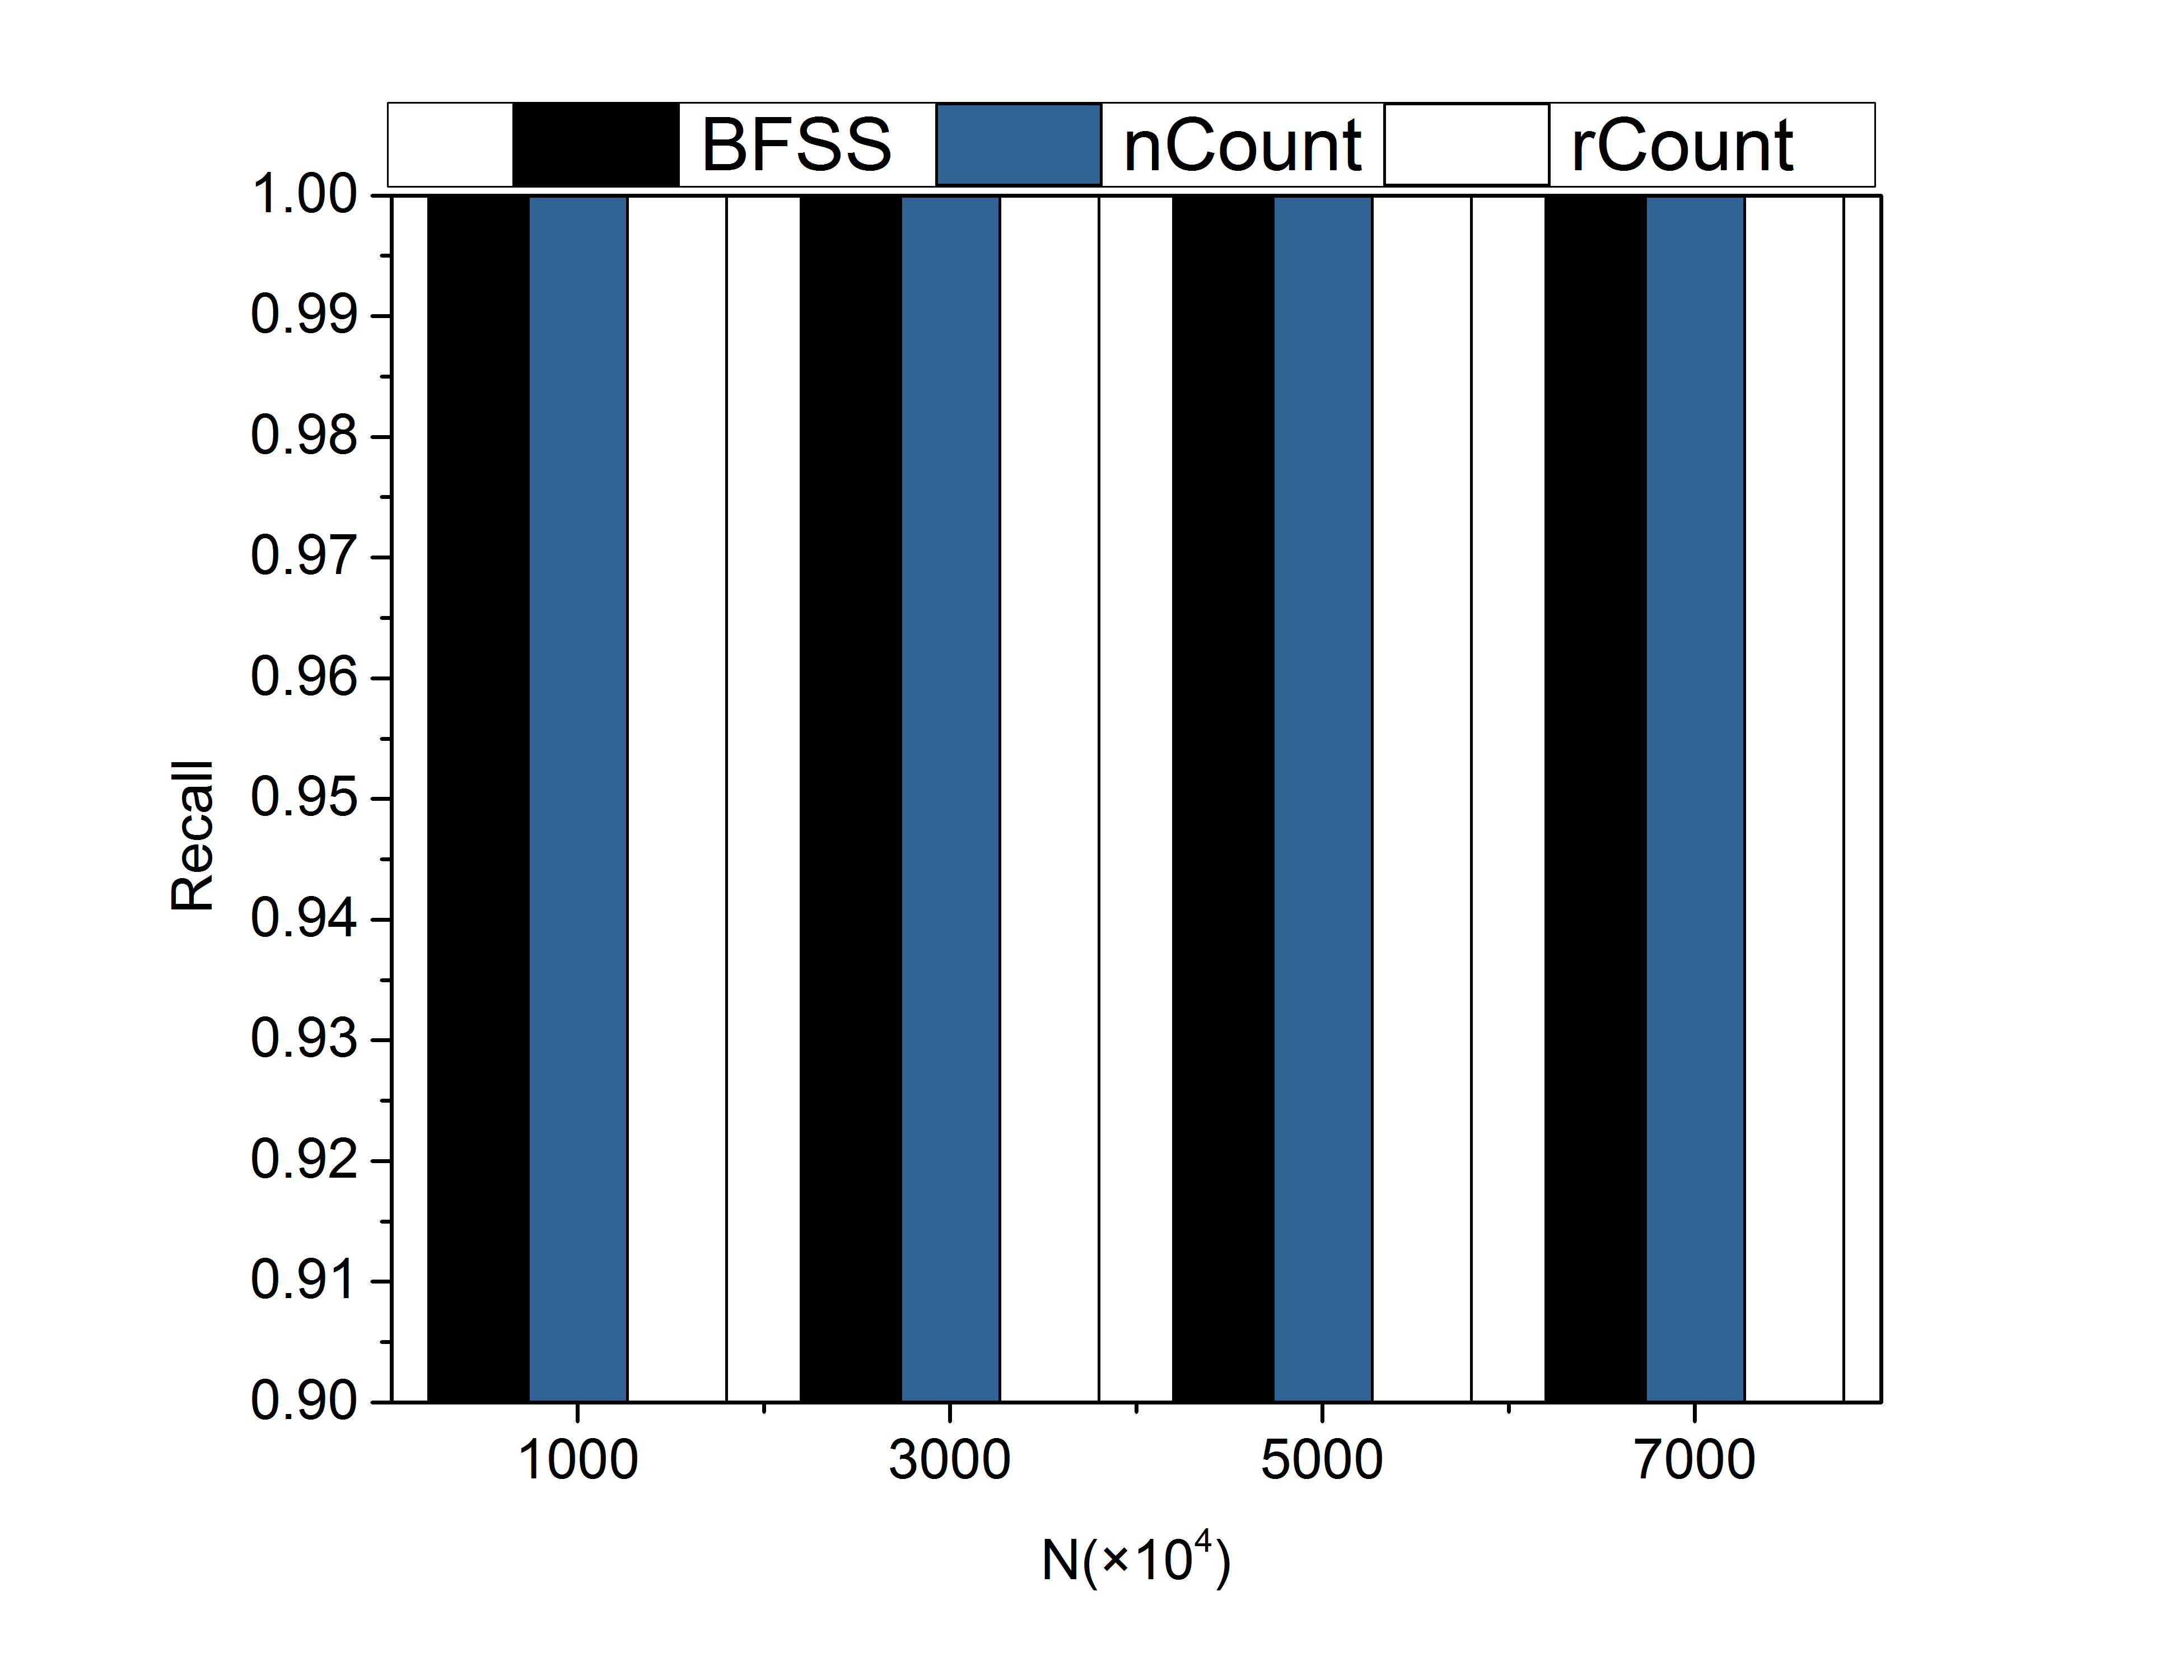
\includegraphics[width=2.6in]{png/001_recall.png}\label{subfig:001_recall}}
	\end{minipage}
	\begin{minipage}{0.31\linewidth}
		\centering
		\subfloat[Recall for $0.2\%$-BLFE]{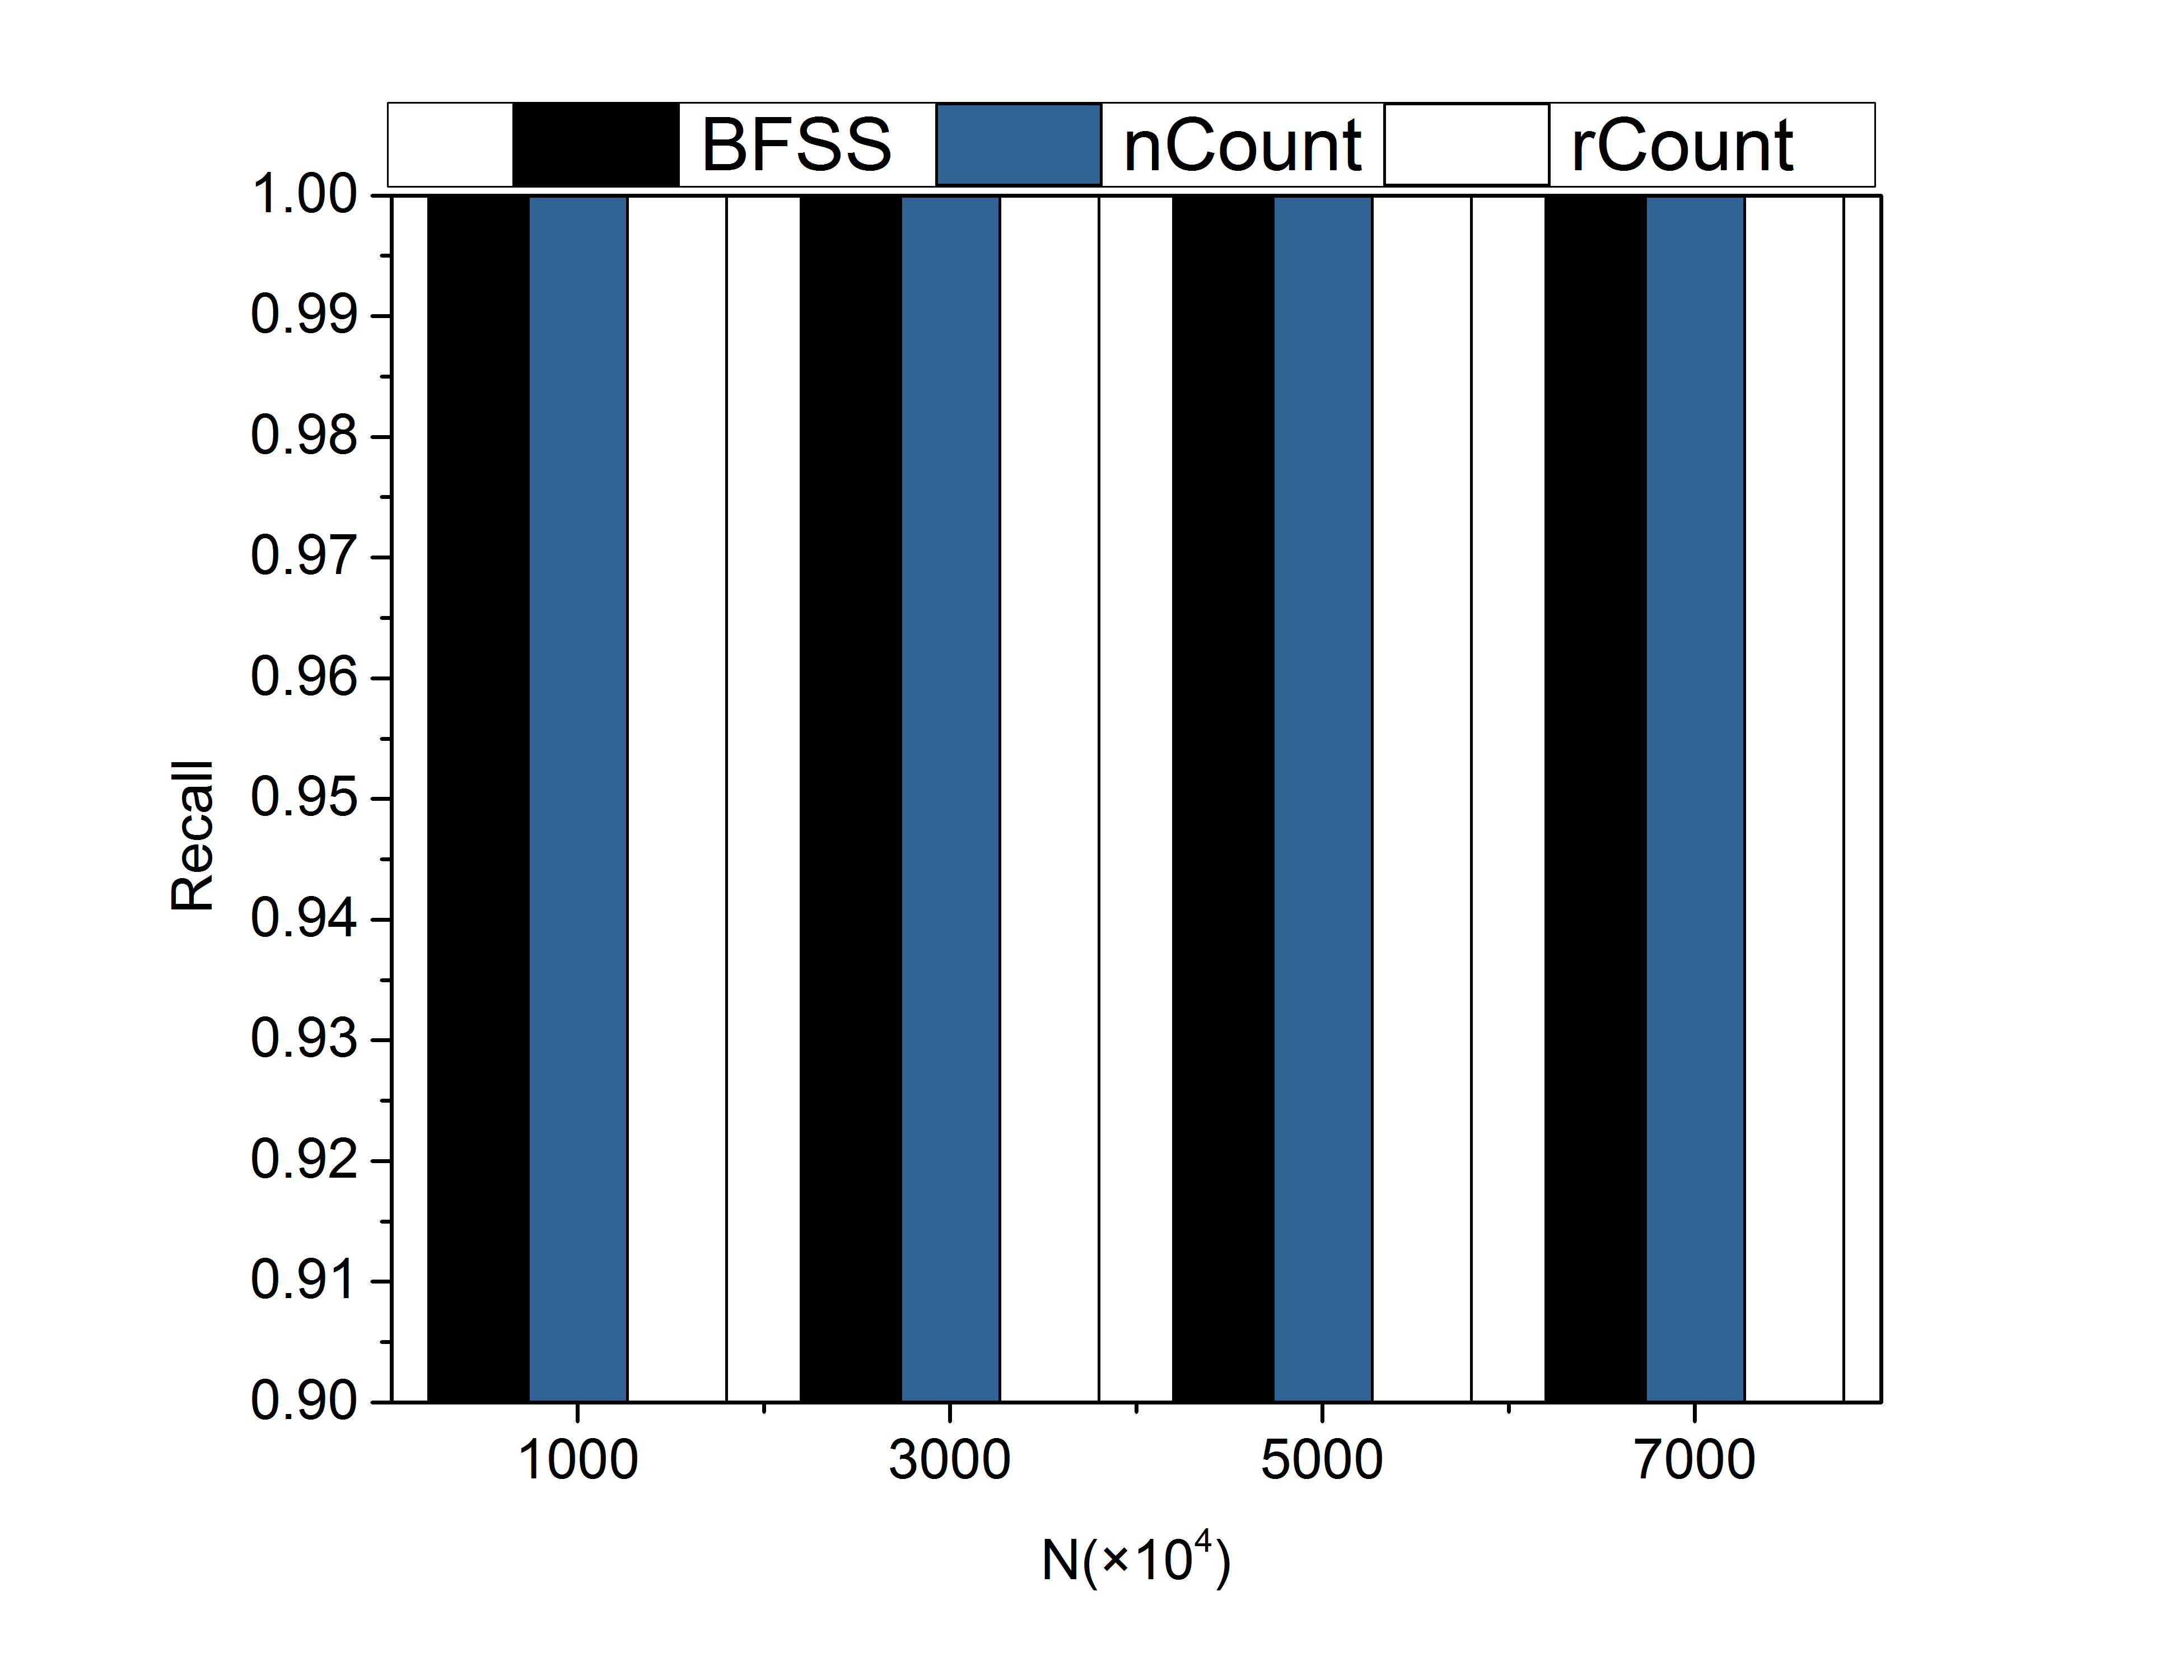
\includegraphics[width=2.6in]{png/0002_recall.png}\label{subfig:0002_recall}}
	\end{minipage}
	\begin{minipage}{0.31\linewidth}
		\centering
		\subfloat[Recall for $0.1\%$-BLFE]{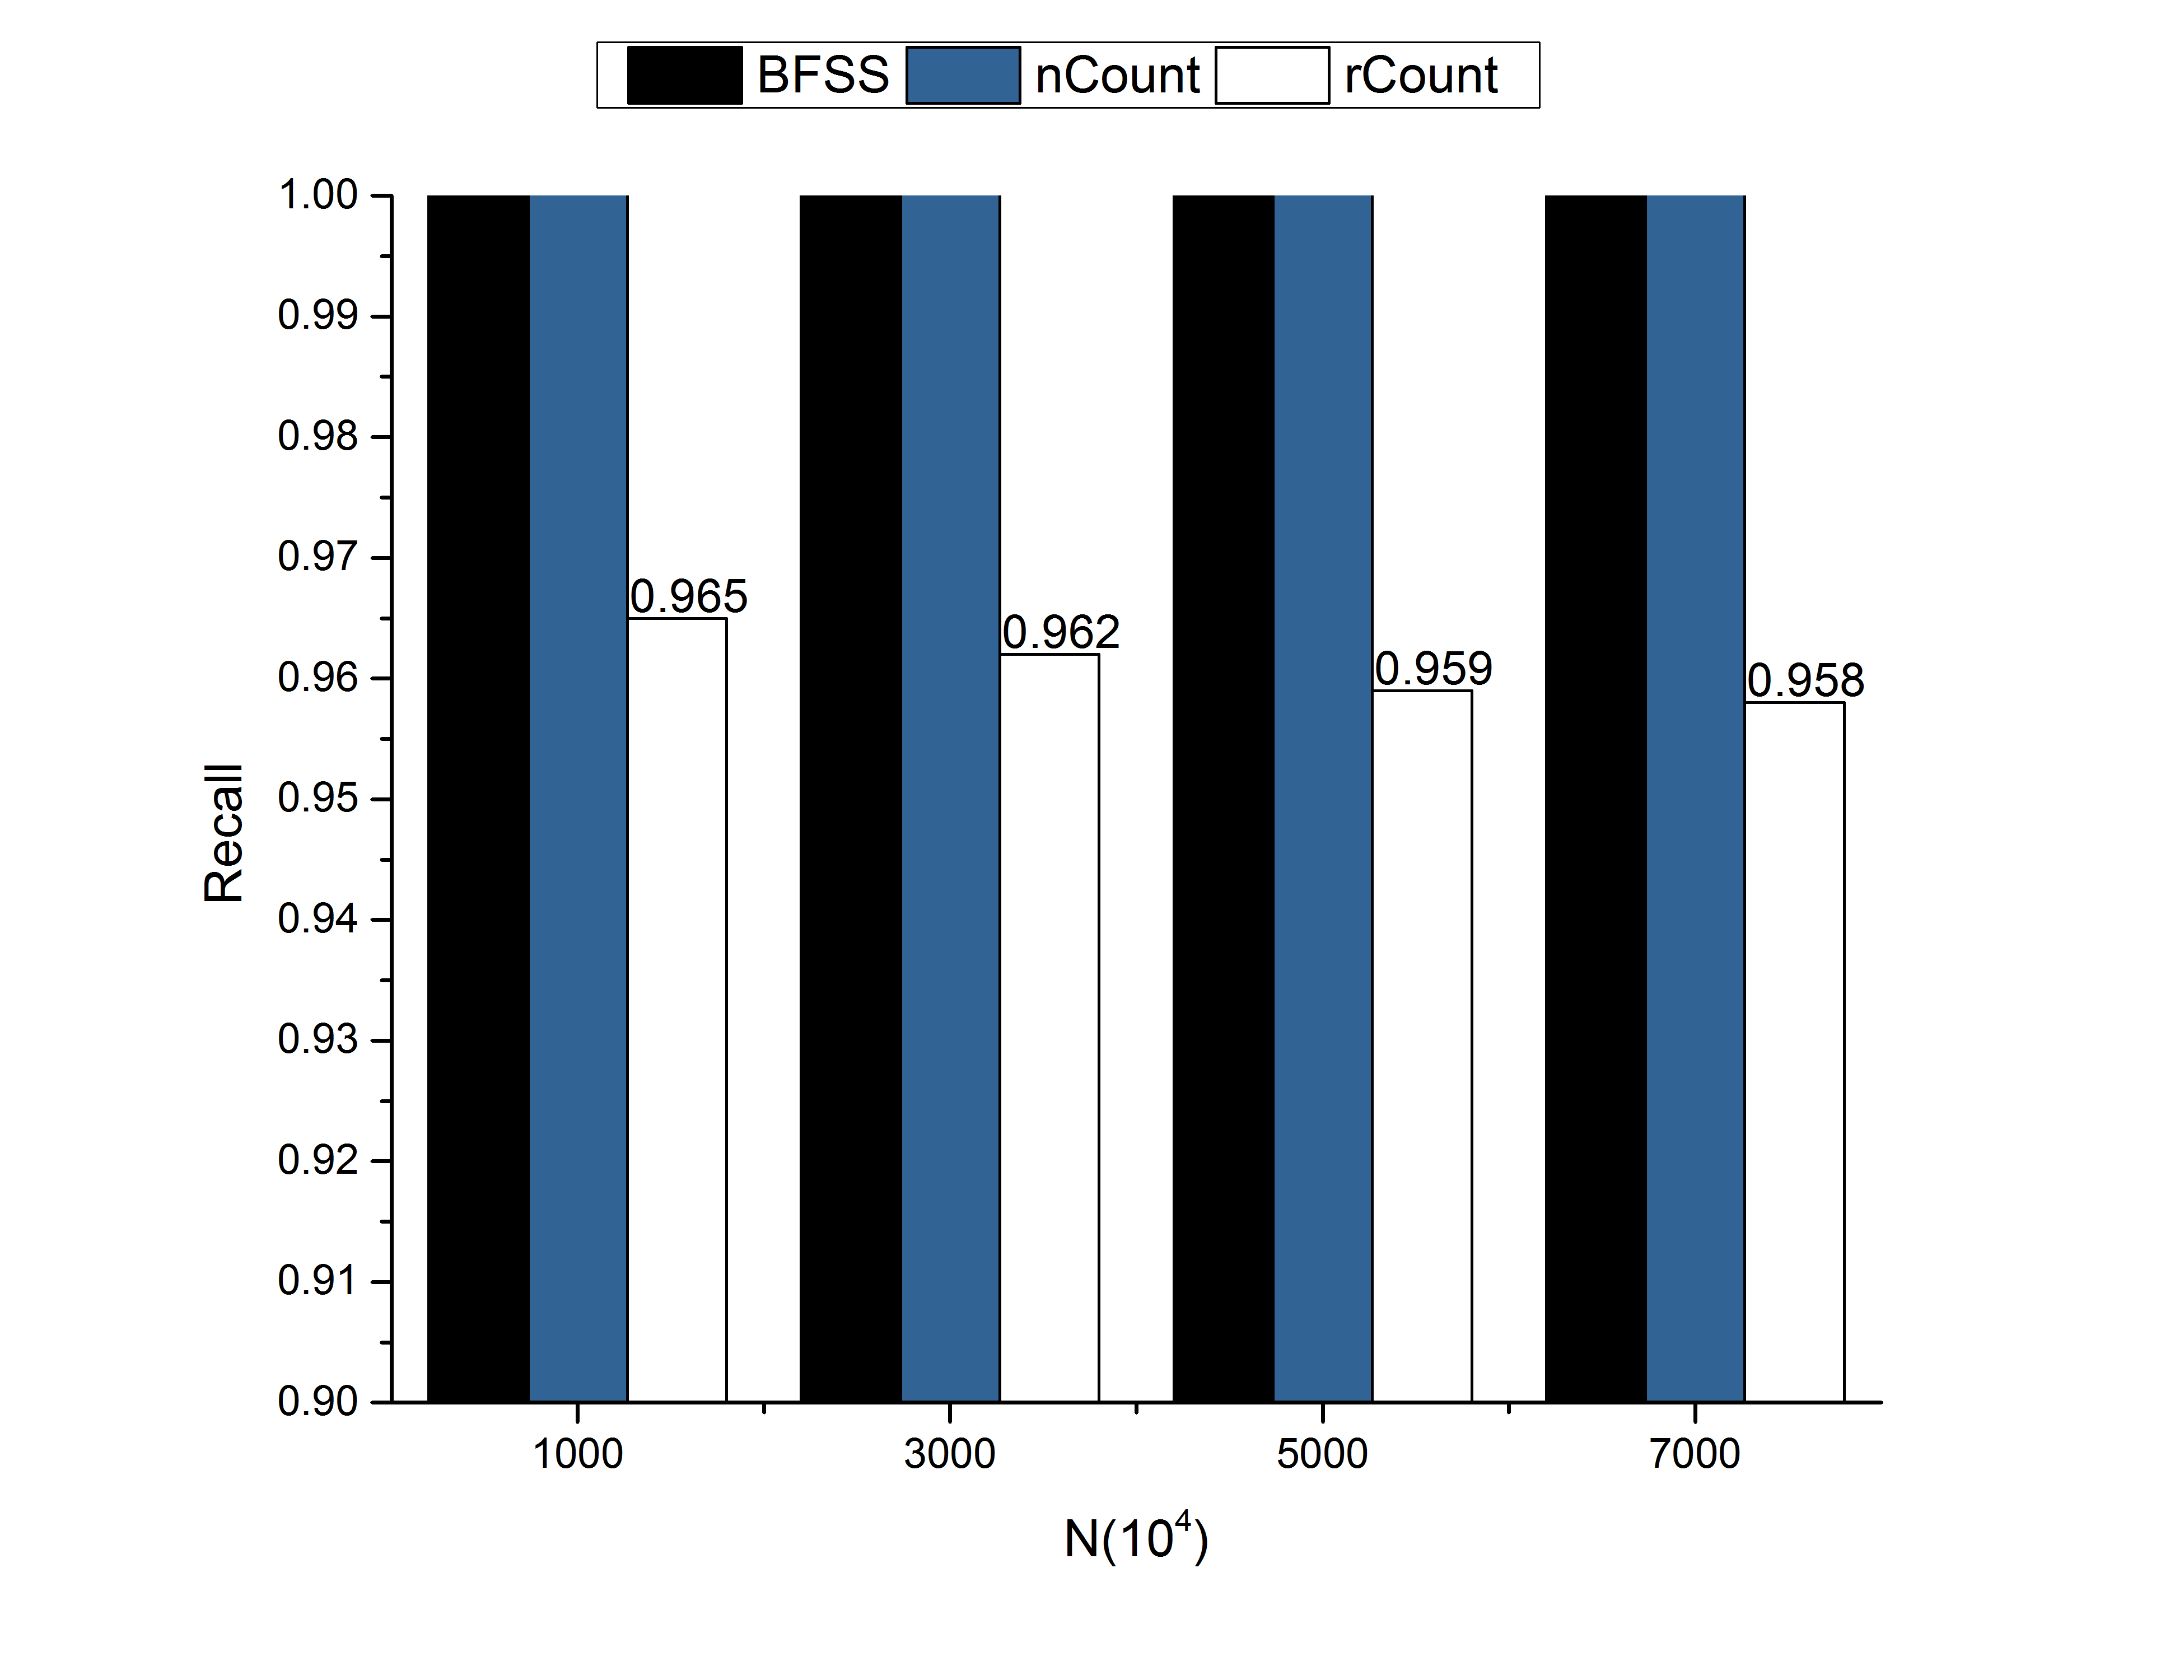
\includegraphics[width=2.6in]{png/recall.png}\label{subfig:0001_recall}}
	\end{minipage}
	
	\begin{minipage}{0.31\linewidth}
		\centering
		\subfloat[Precision for $1\%$-BLFE]{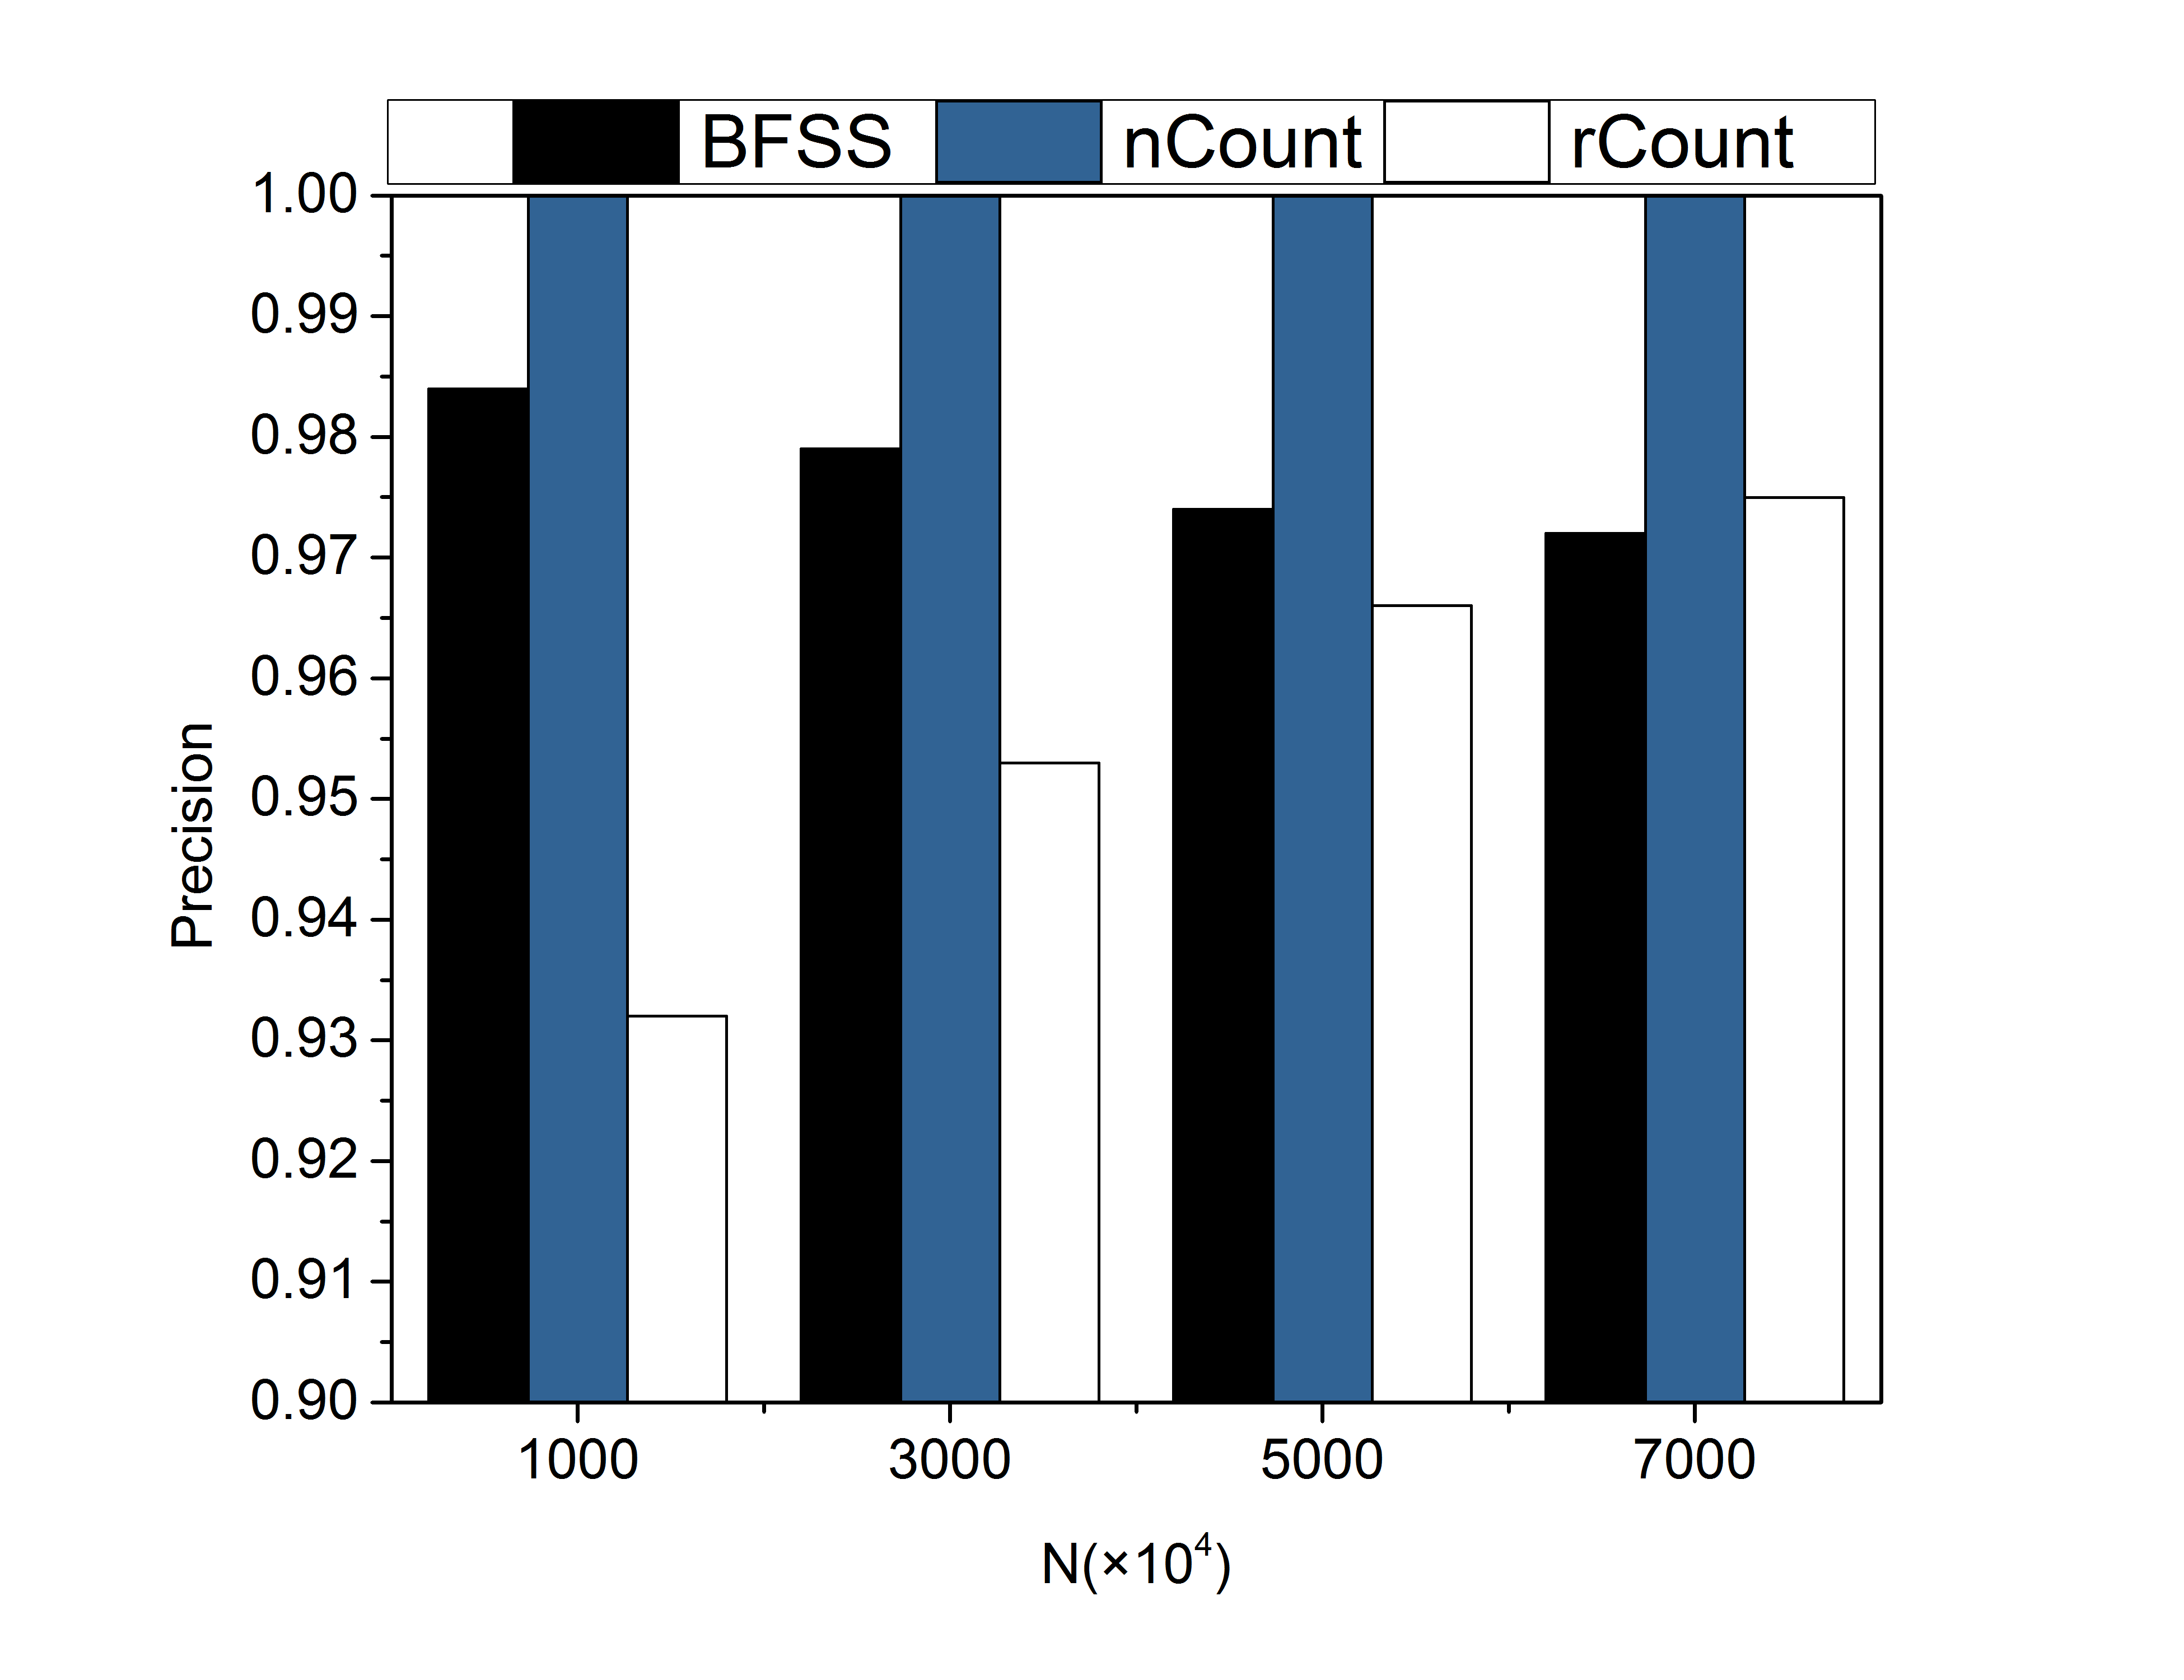
\includegraphics[width=2.6in]{png/001_precision.png}\label{subfig:001_precison}}
	\end{minipage}
	\begin{minipage}{0.31\linewidth}
		\centering
		\subfloat[Precision for $0.2\%$-BLFE]{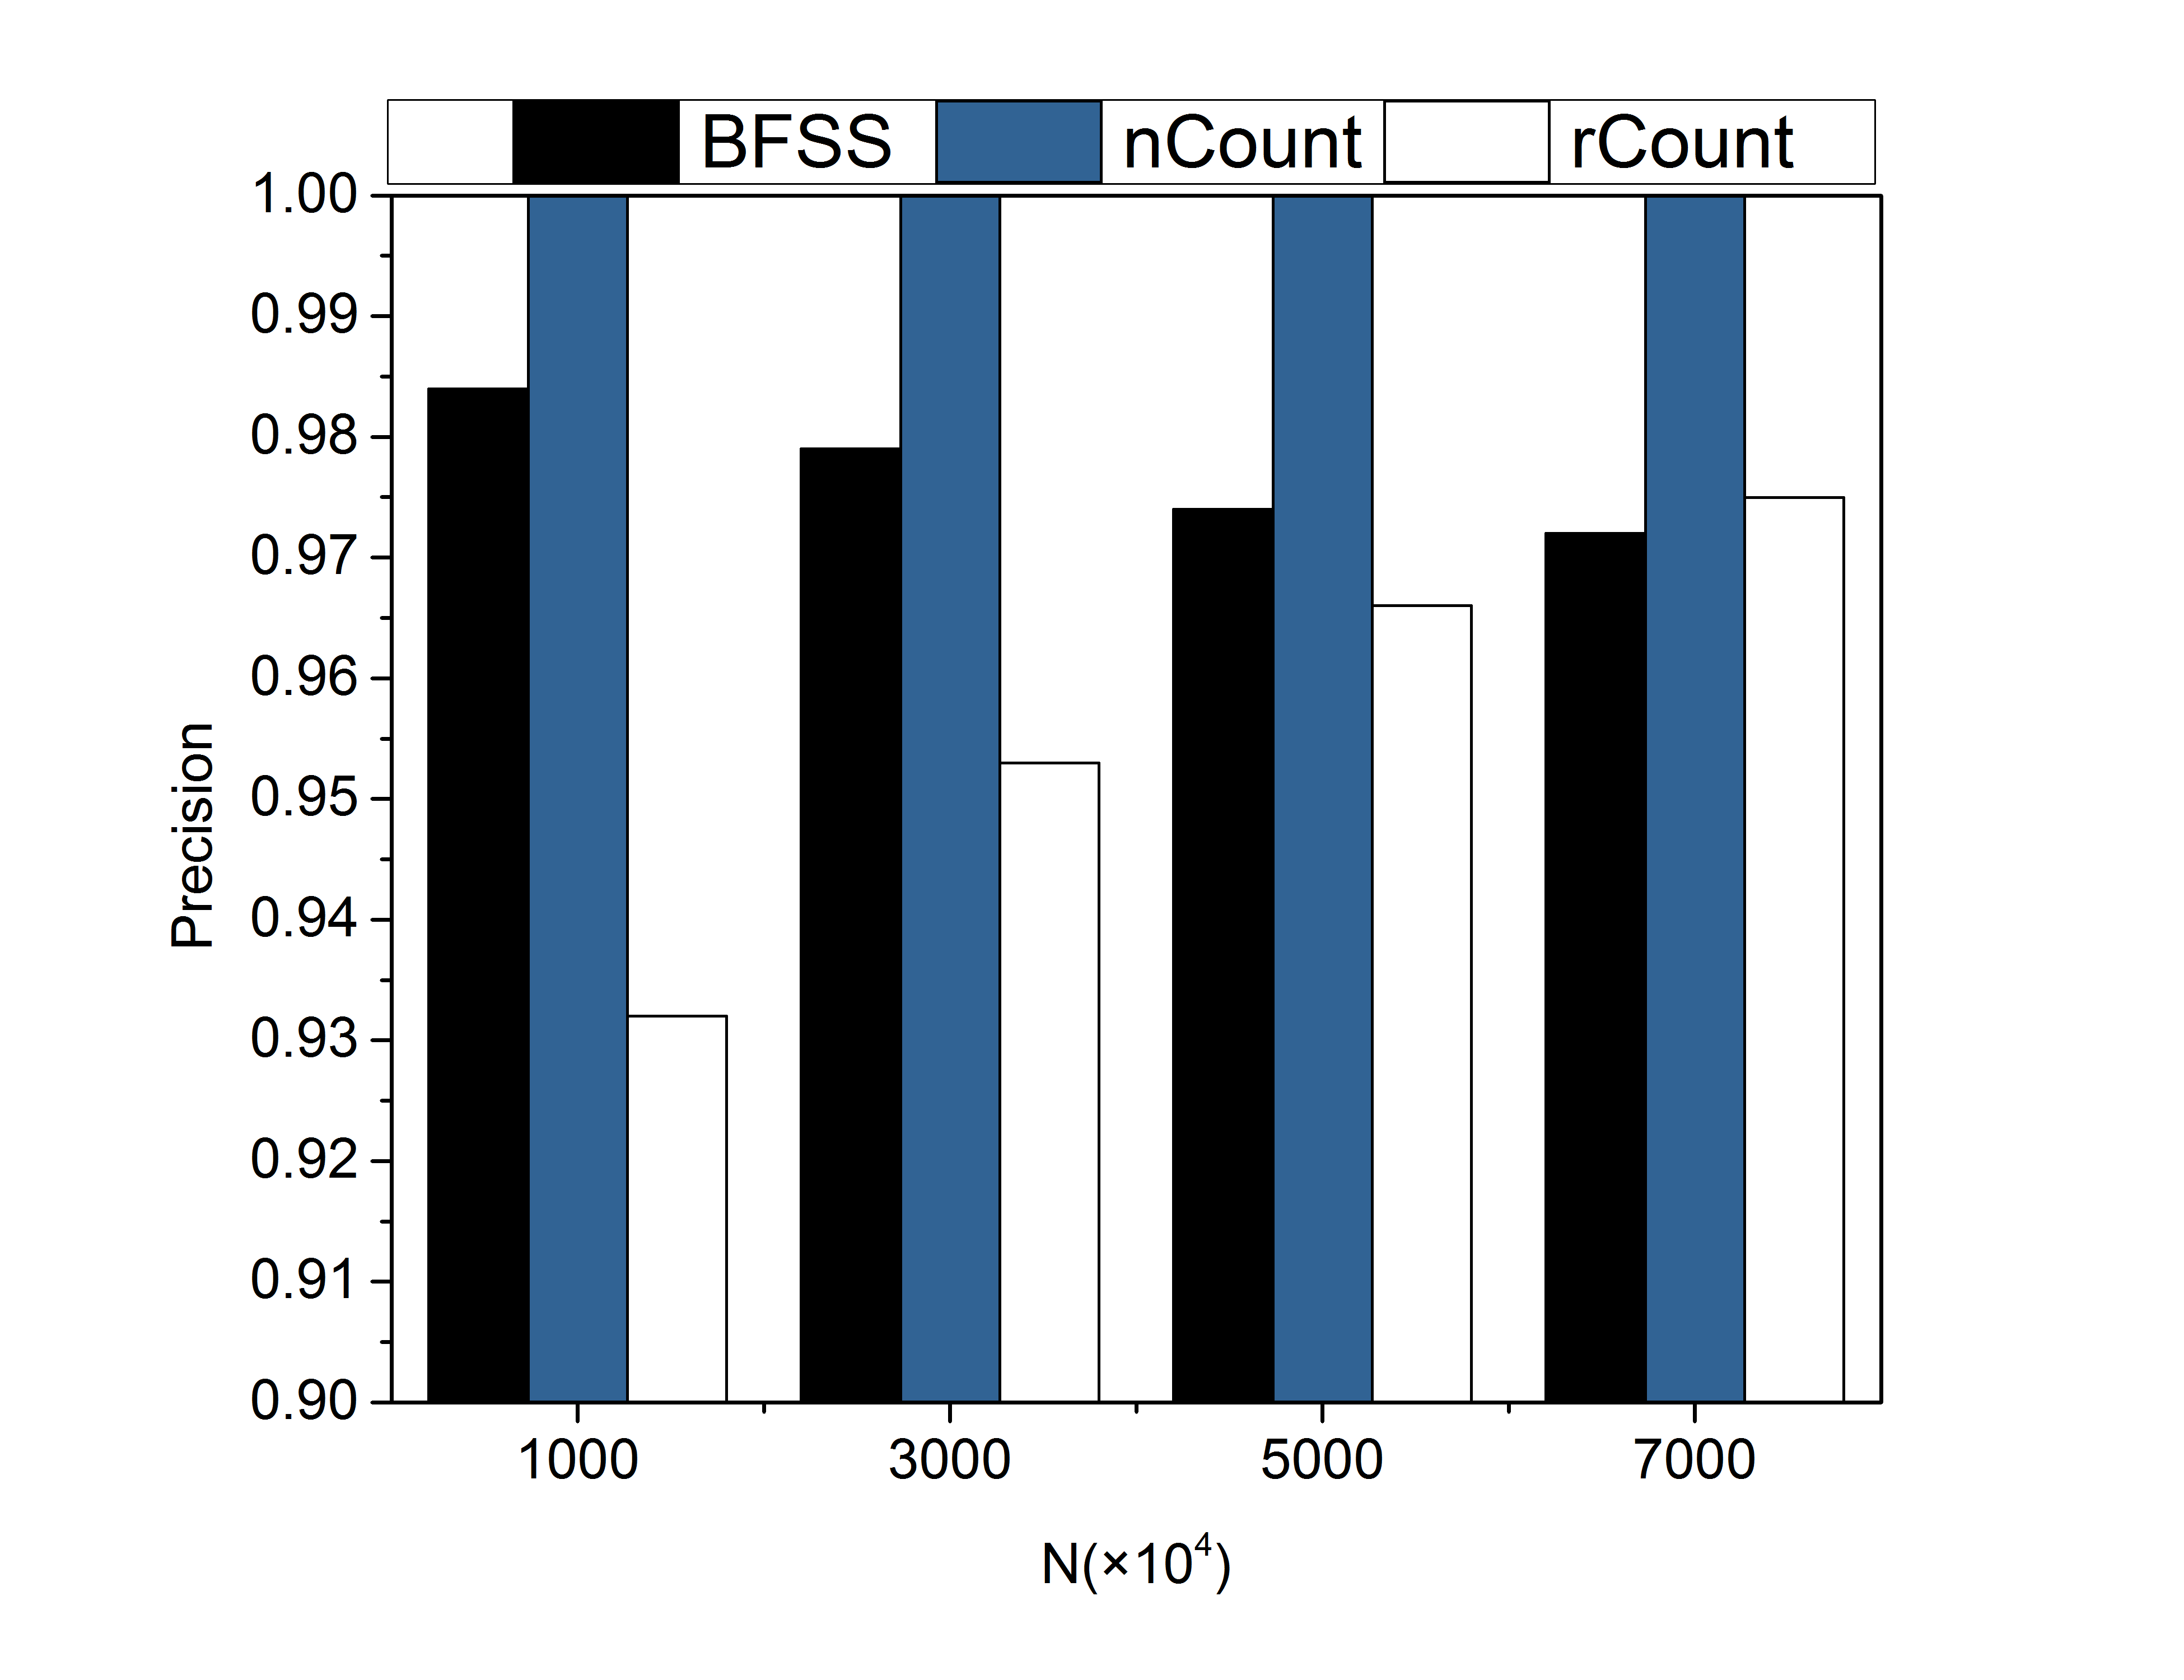
\includegraphics[width=2.6in]{png/0002_precision.png}\label{subfig:0002_precison}}
	\end{minipage}
	\begin{minipage}{0.31\linewidth}
		\centering
		\subfloat[Precision for $0.1\%$-BLFE]{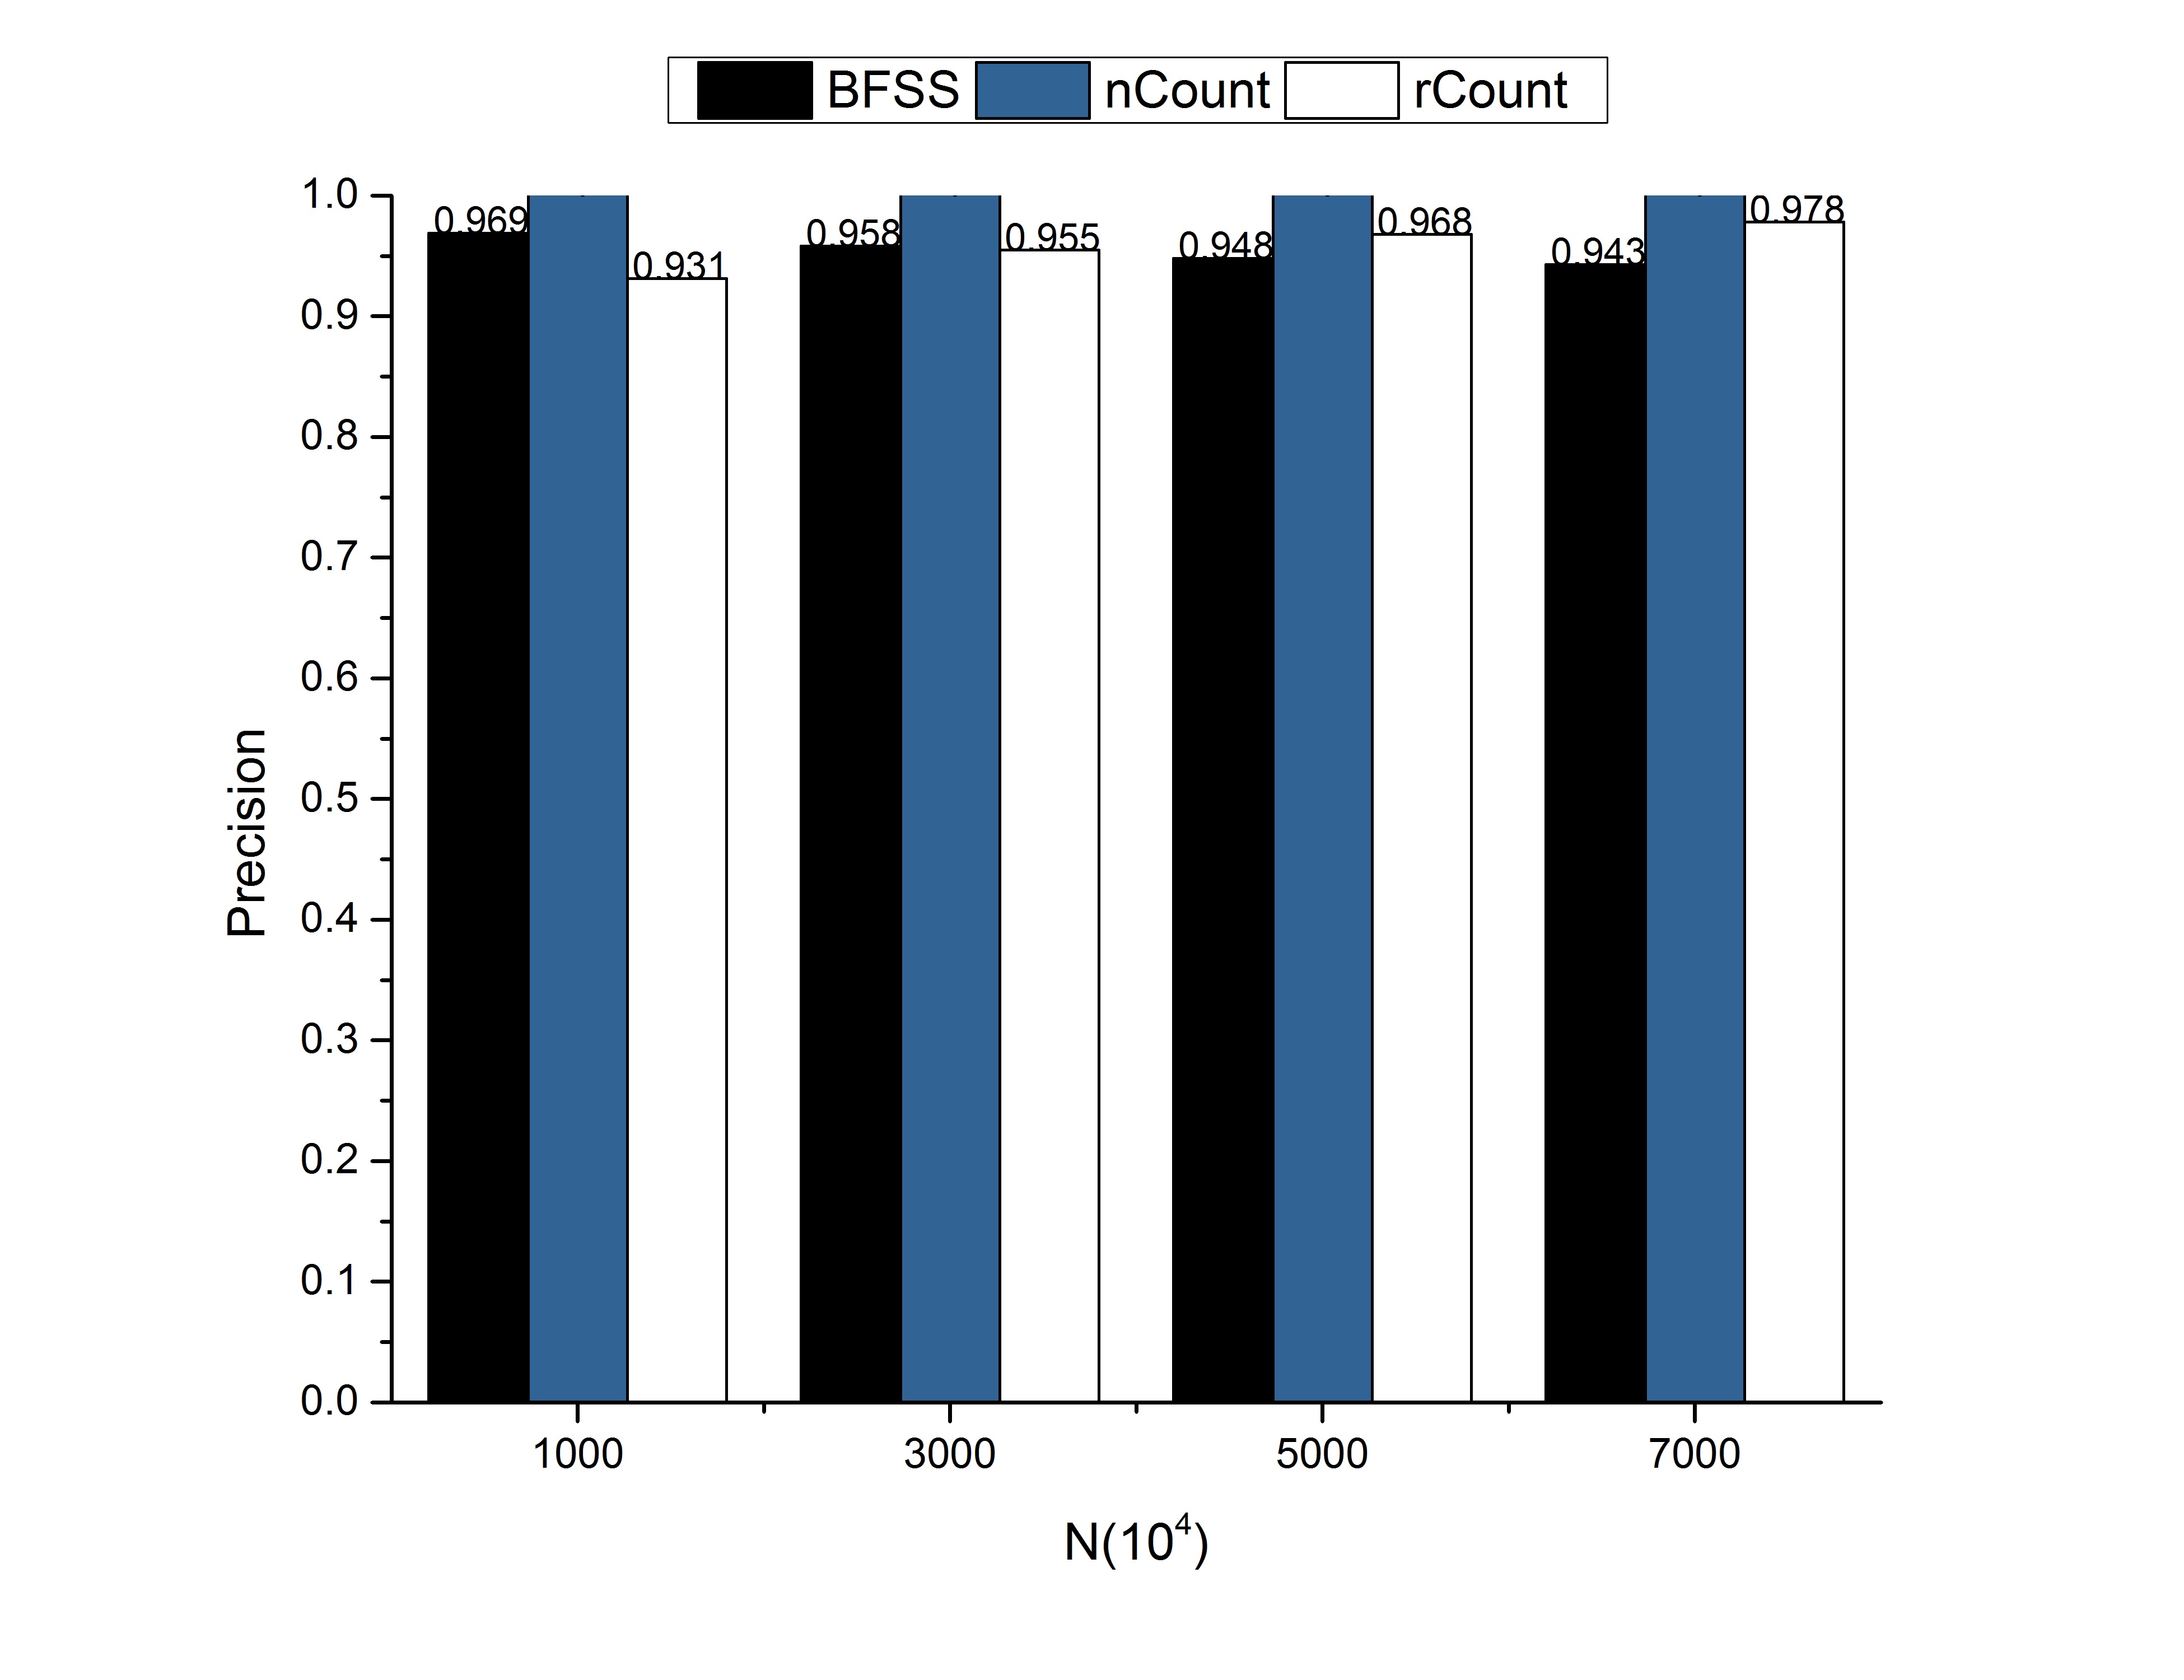
\includegraphics[width=2.6in]{png/precision.png}\label{subfig:0001_precison}}
	\end{minipage}
	
	\begin{minipage}{0.31\linewidth}
		\centering
		\subfloat[$F_1$ for $1\%$-BLFE]{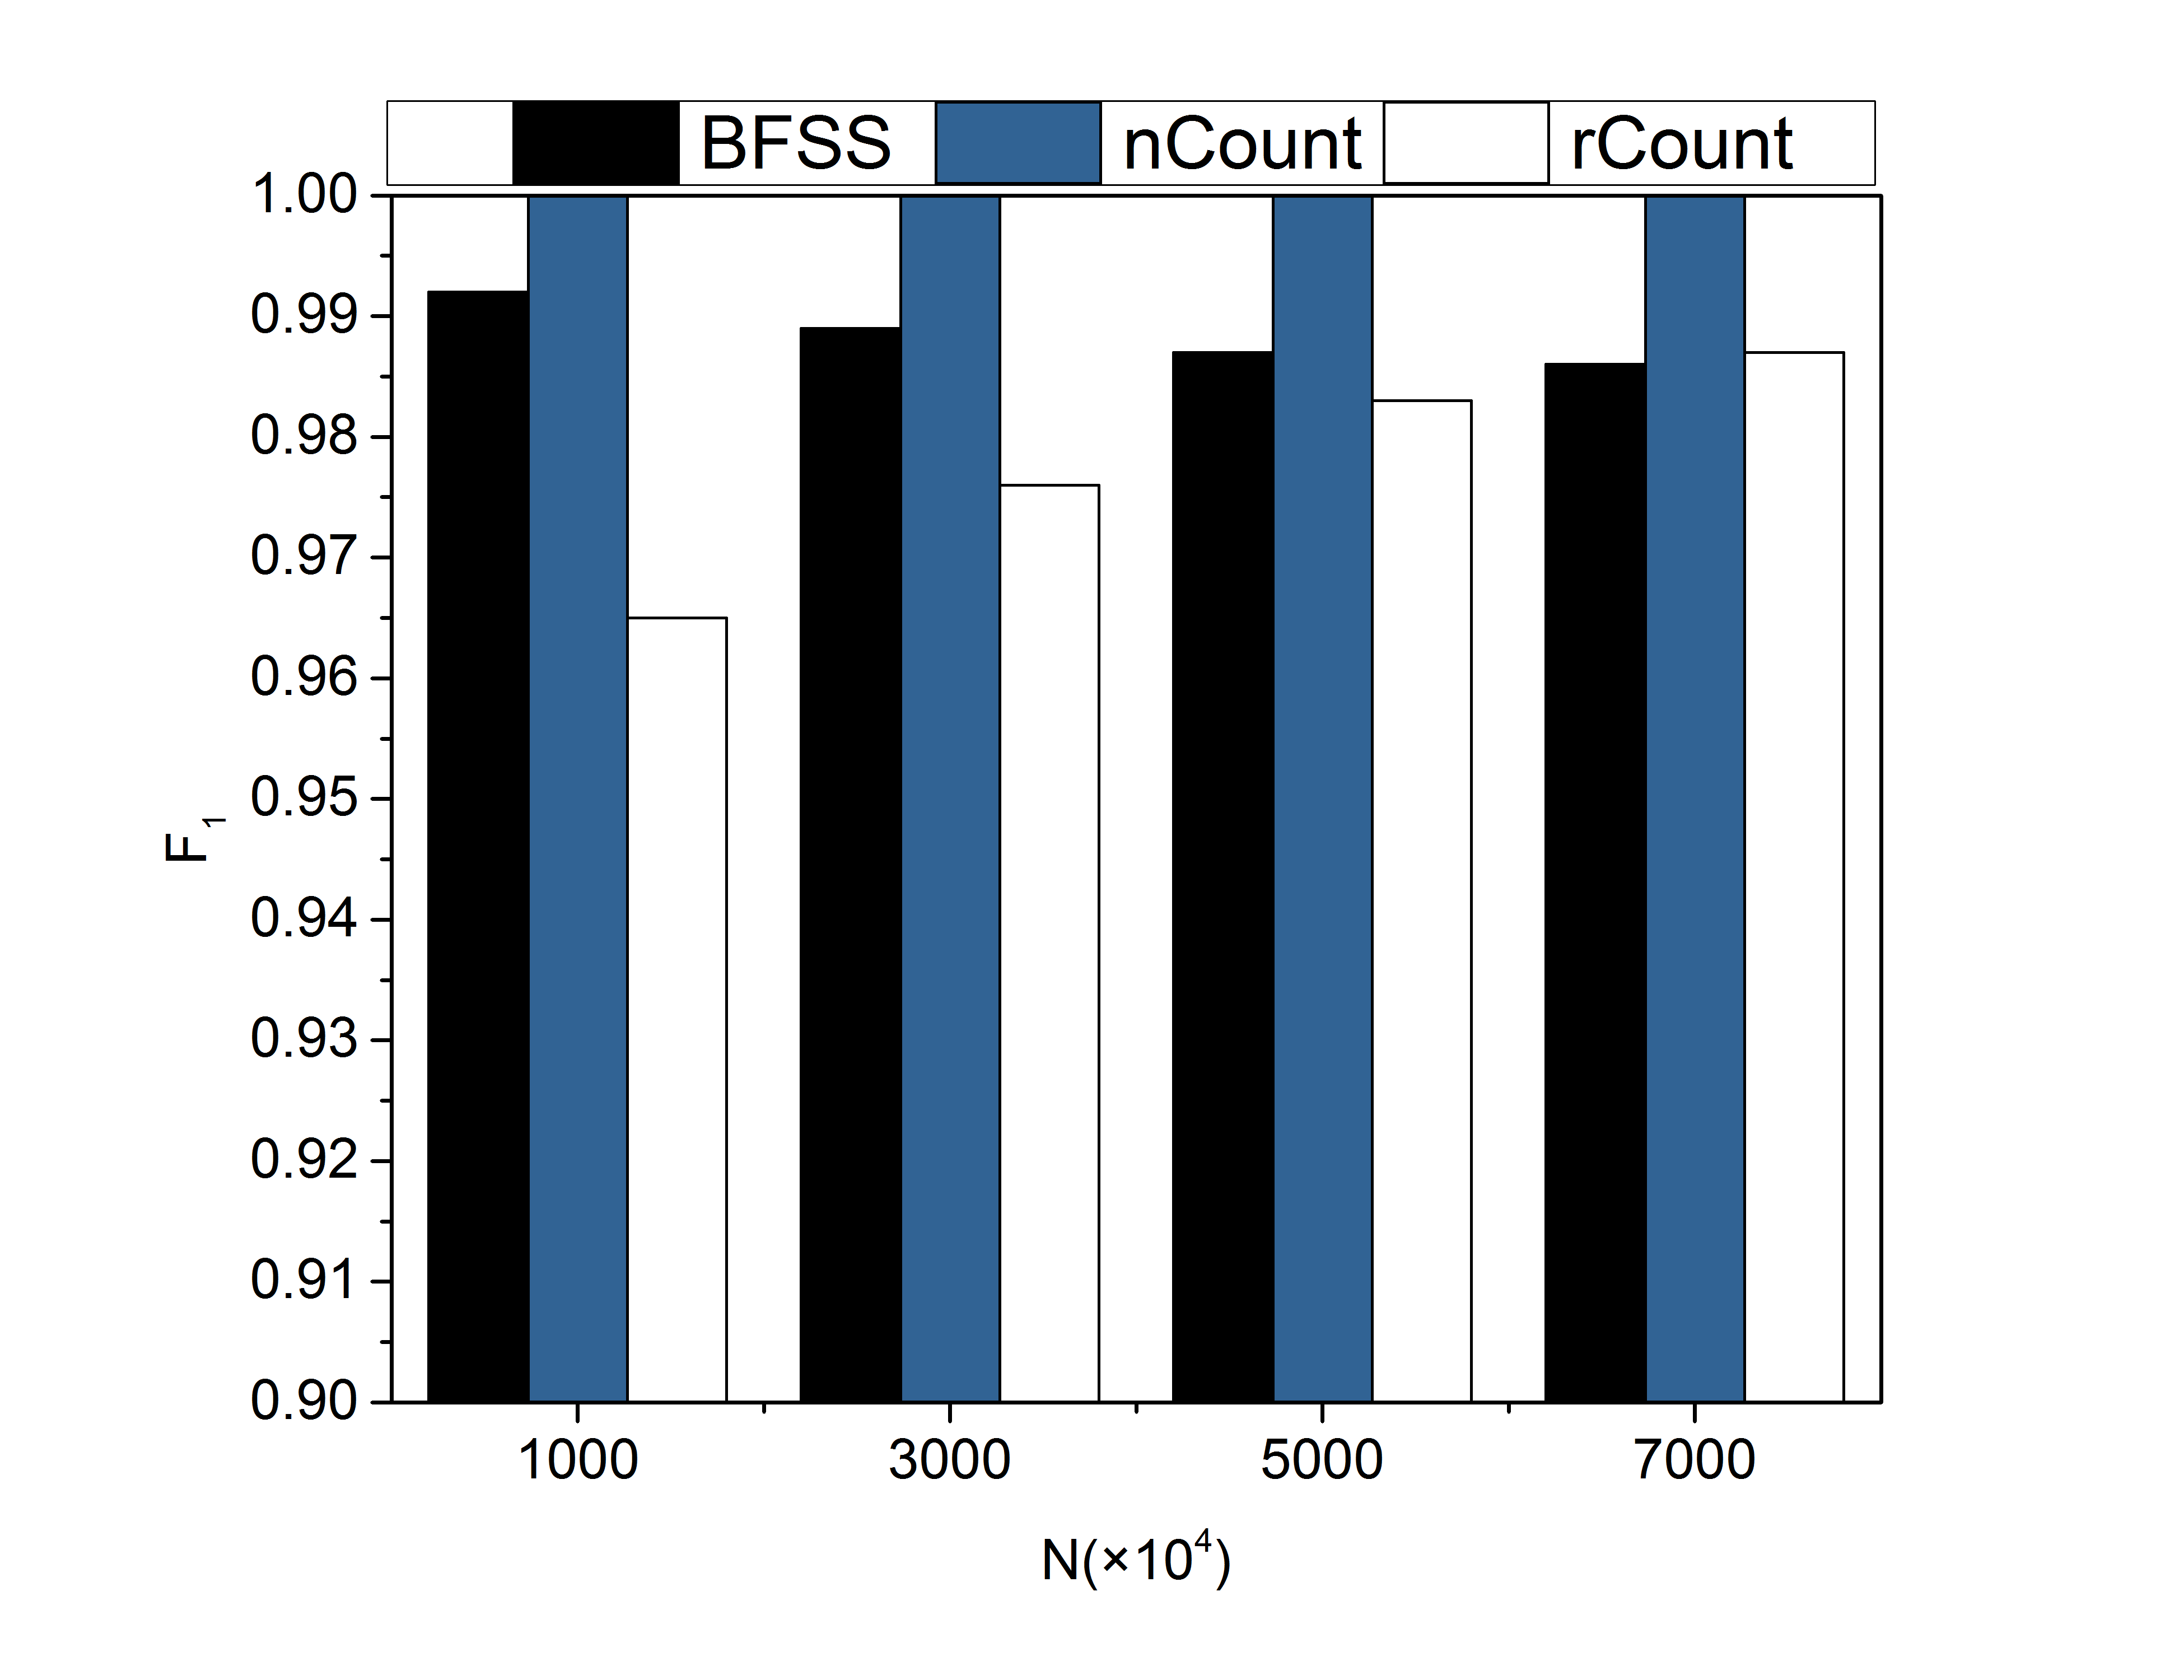
\includegraphics[width=2.6in]{png/001_f1.png}\label{subfig:001_f1}}
	\end{minipage}
	\begin{minipage}{0.31\linewidth}
		\centering
		\subfloat[$F_1$ for $0.2\%$-BLFE]{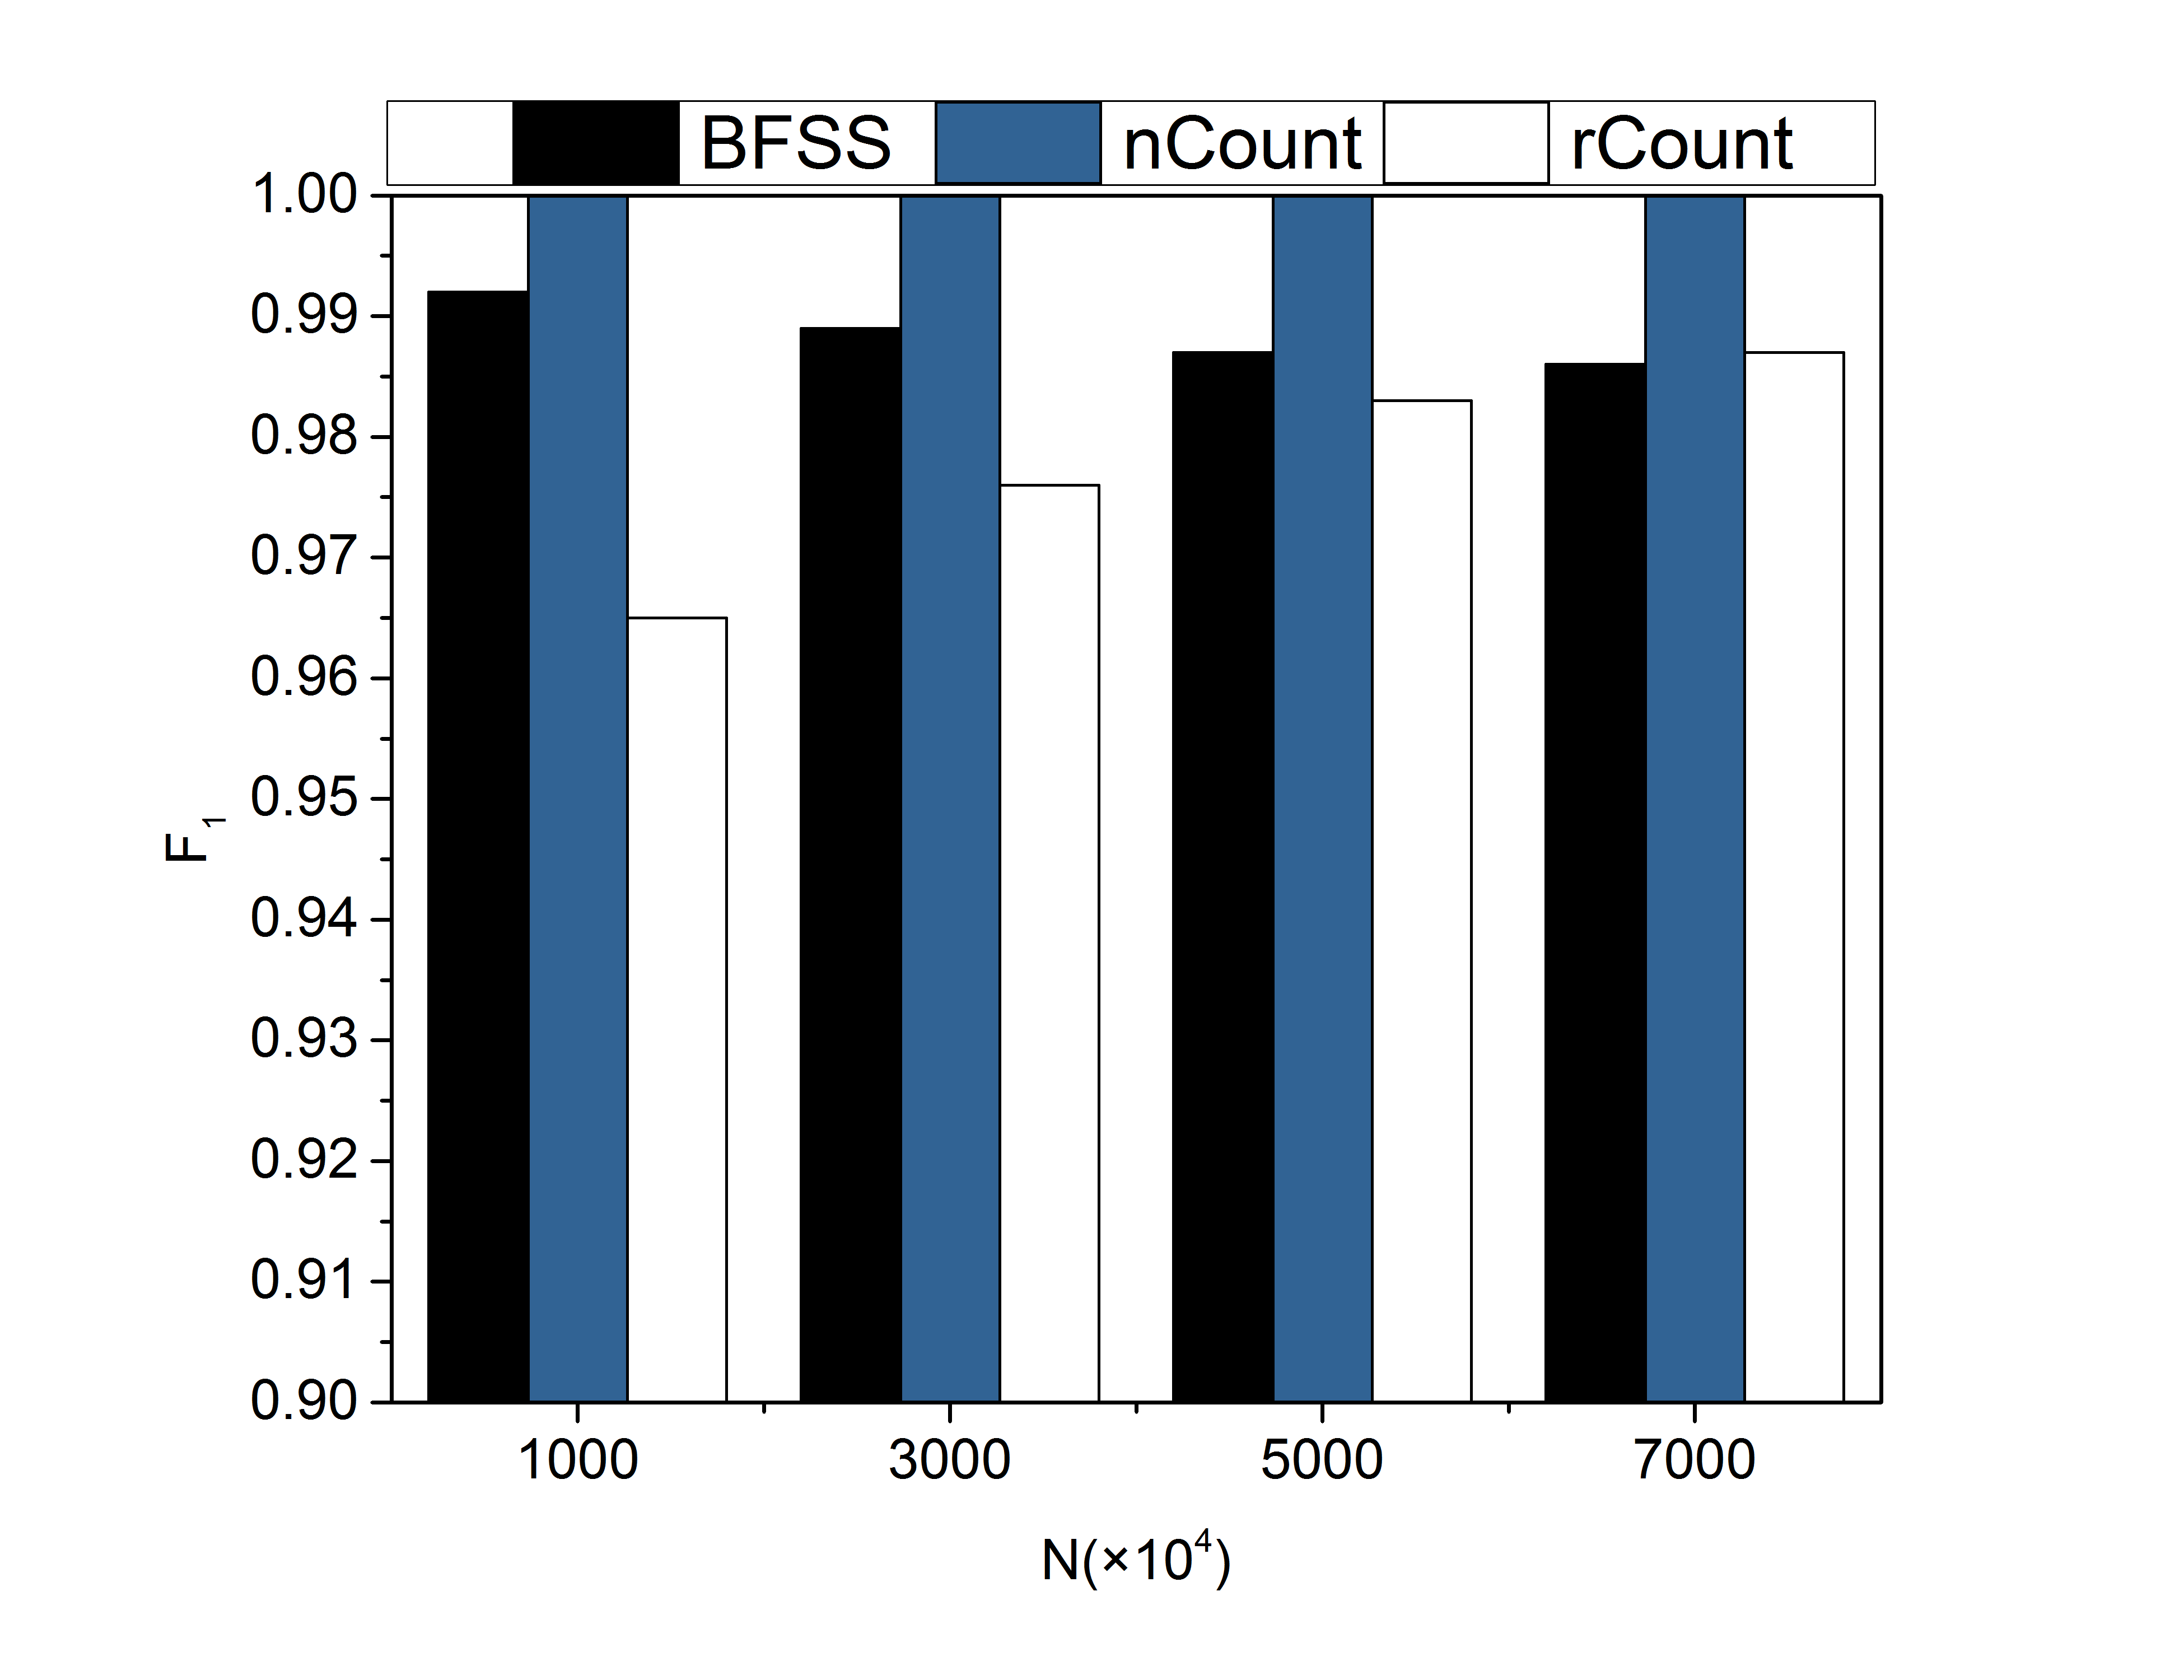
\includegraphics[width=2.6in]{png/0002_f1.png}\label{subfig:0002_f1}}
	\end{minipage}
	\begin{minipage}{0.31\linewidth}
		\centering
		\subfloat[$F_1$ for $0.1\%$-BLFE]{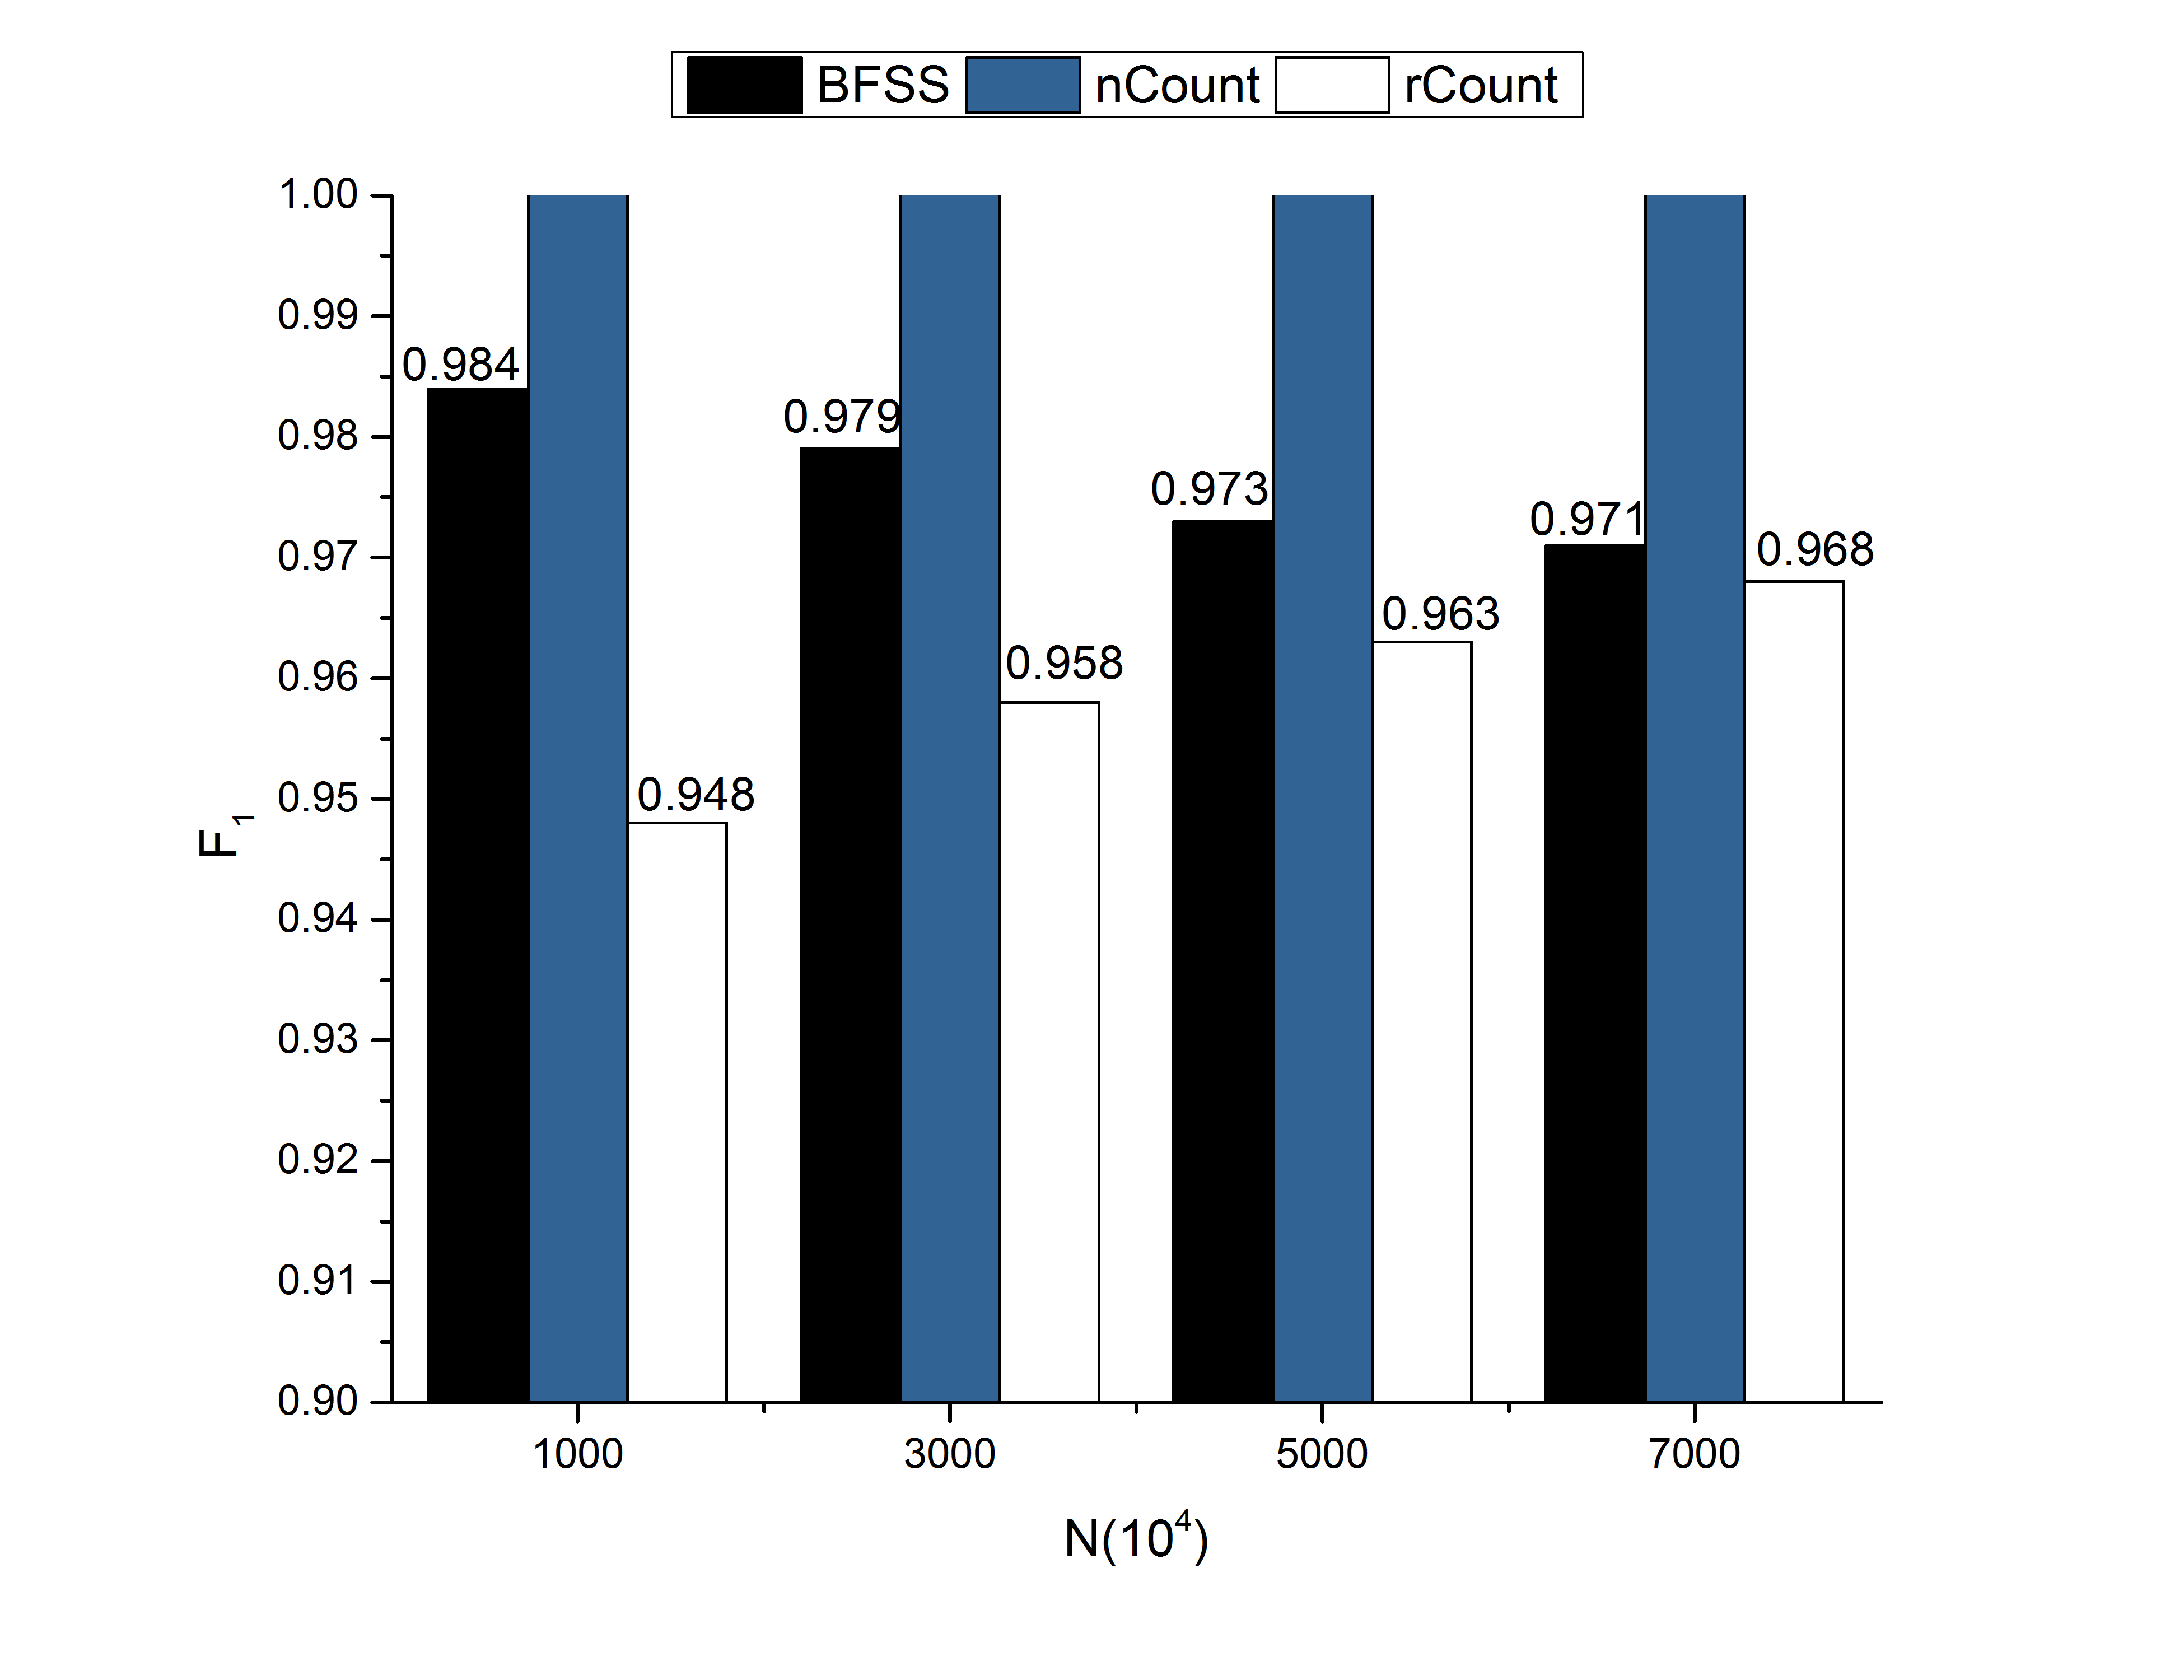
\includegraphics[width=2.6in]{png/f1.png}\label{subfig:0001_f1}}
	\end{minipage}
	
	\begin{minipage}{0.31\linewidth}
		\centering
		\subfloat[Space for $1\%$-BLFE]{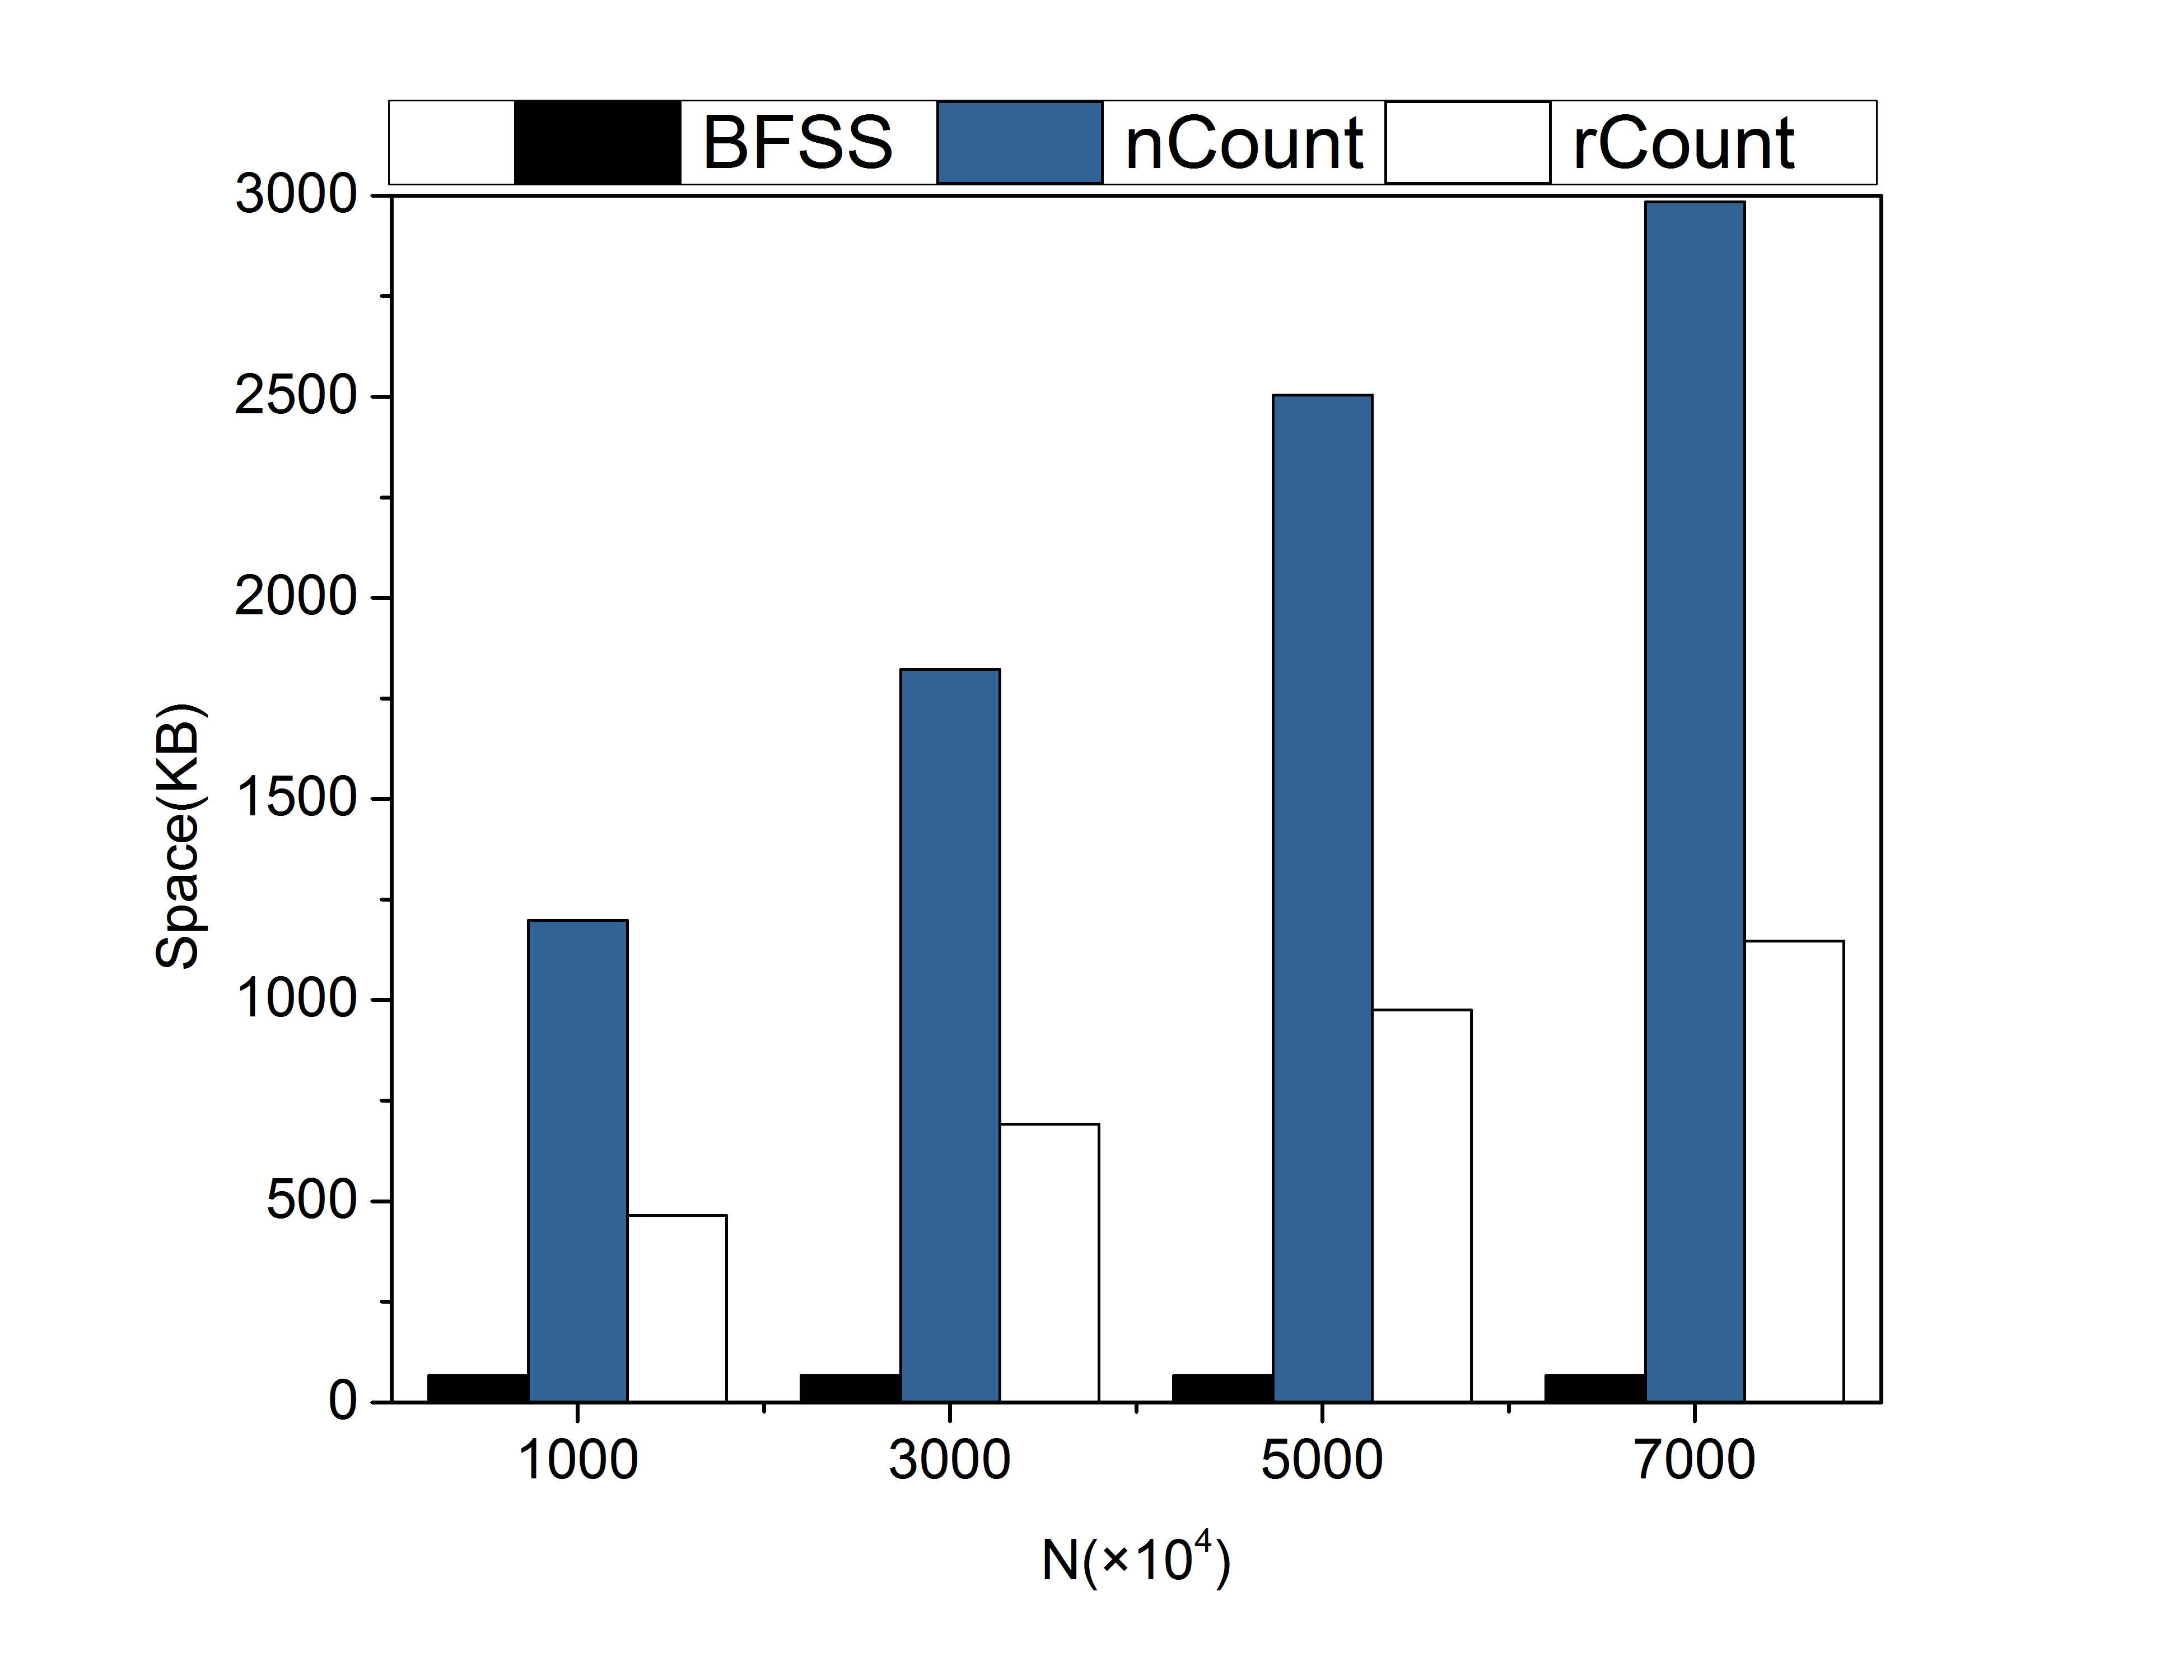
\includegraphics[width=2.6in]{png/001_space.png}\label{subfig:001_space}}
	\end{minipage}
	\begin{minipage}{0.31\linewidth}
		\centering
		\subfloat[Space for $0.2\%$-BLFE]{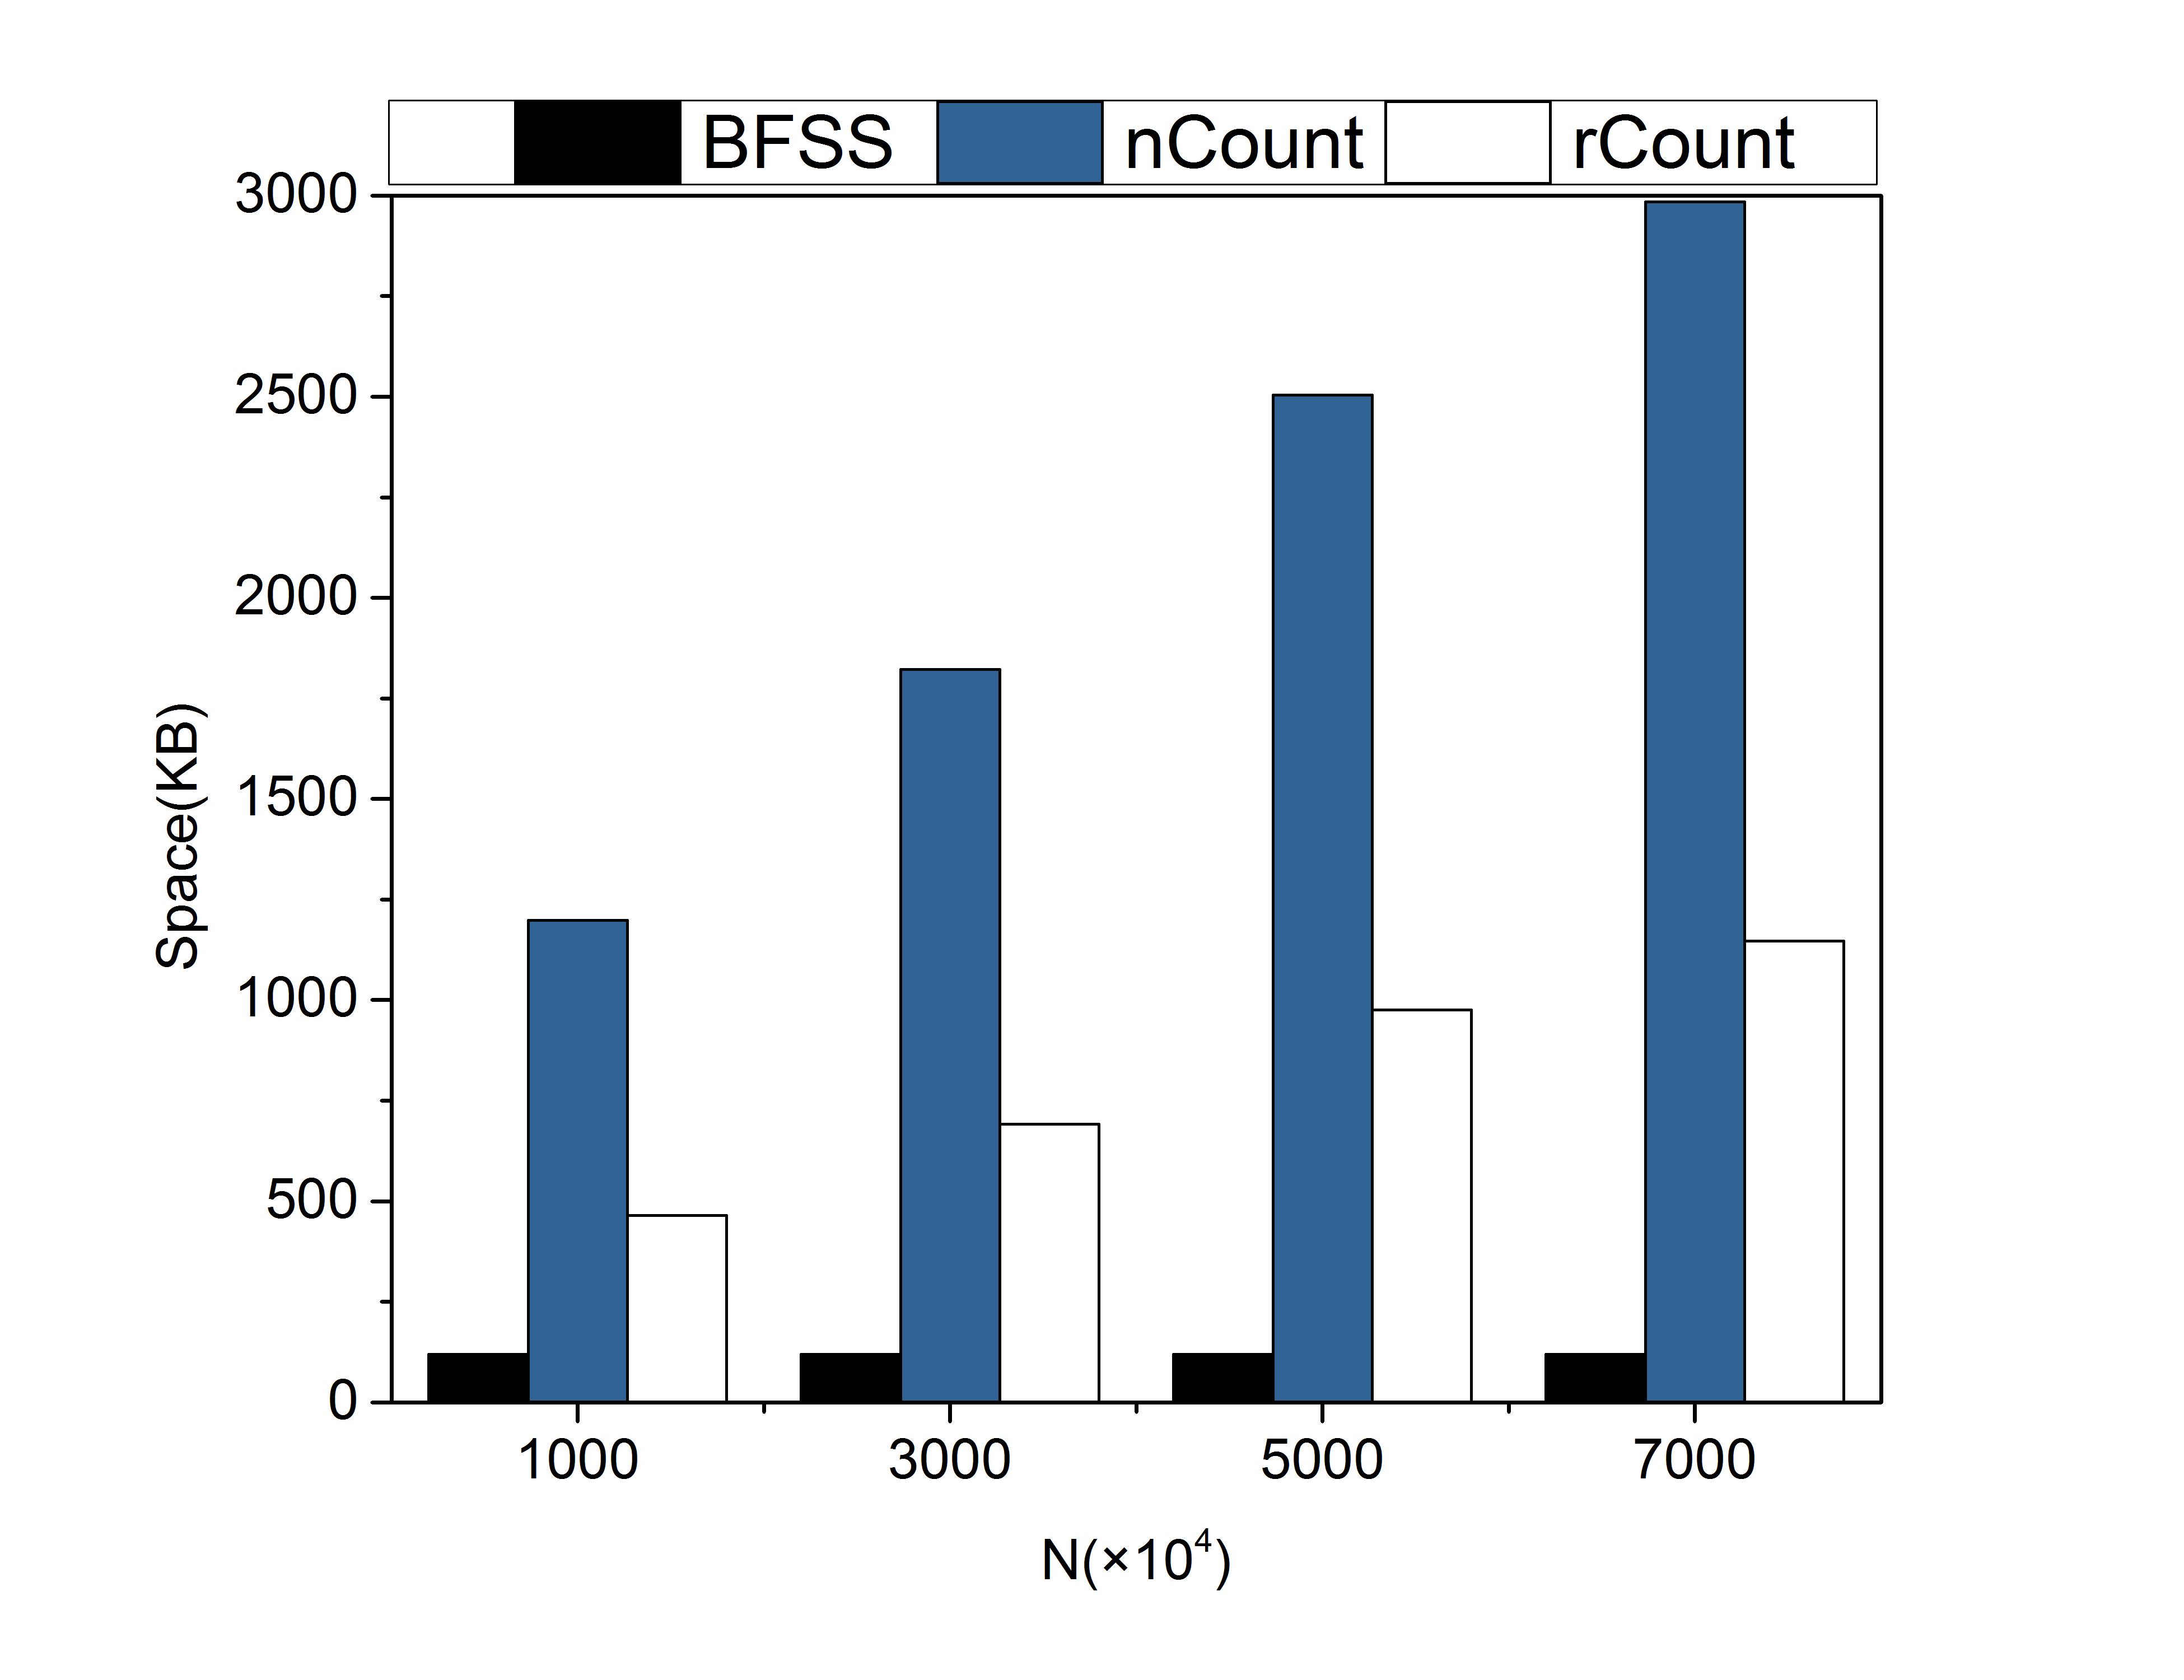
\includegraphics[width=2.6in]{png/0002_space.png}\label{subfig:0002_space}}
	\end{minipage}
	\begin{minipage}{0.31\linewidth}
	   \centering
	   \subfloat[Space for $0.1\%$-BLFE]{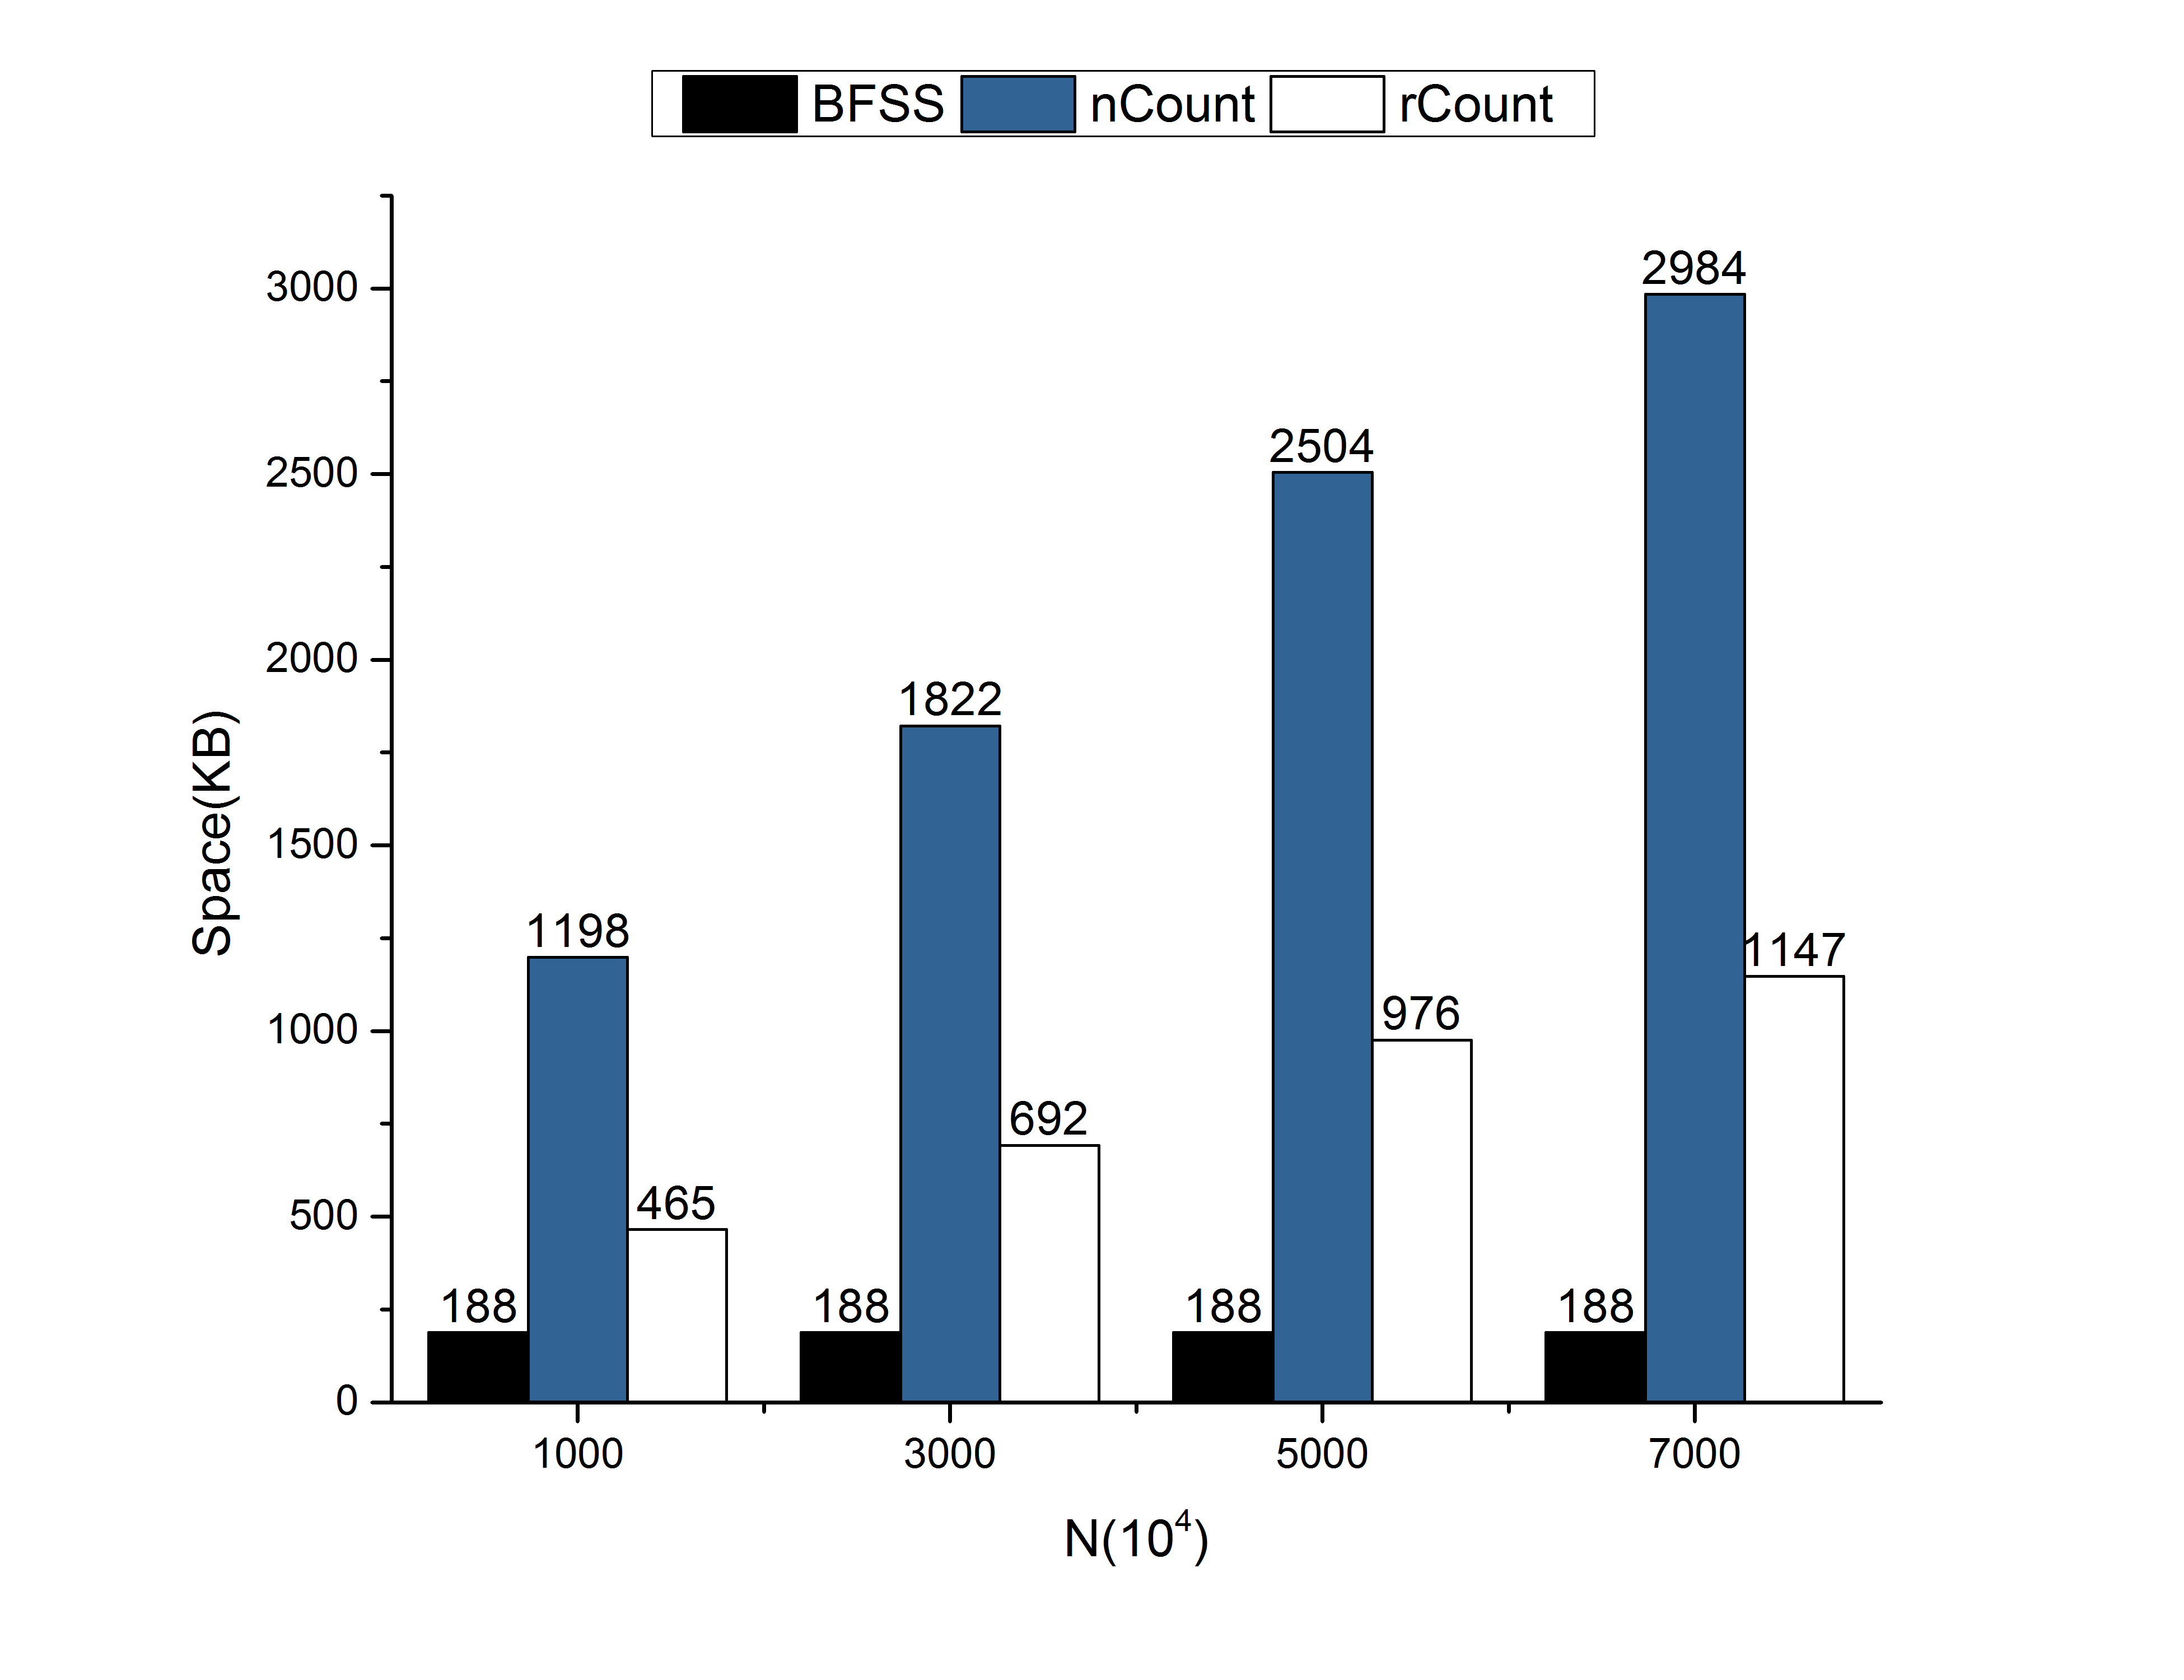
\includegraphics[width=2.6in]{png/space.png}\label{subfig:0001_space}}
	\end{minipage}
	\caption{ Performance Comparison between \emph{BFSS}, \emph{nCount} and \emph{rCount} on $W$ - Varying $s,\epsilon$ and $N$ }
	\label{fig:performance comparison of BFSS}
\end{figure*}

\begin{table*}[!t] 
\centering 
\caption{ Performance of \emph{BFSS} Using Real Data - Varying $s$, $\epsilon$, $K$ and $N$ } 
\label{tab:bfss} 
\begin{IEEEeqnarraybox}[\IEEEeqnarraystrutmode\IEEEeqnarraystrutsizeadd{2pt}{0pt}]{v/c/Vx/c/Vx/c/Vx/c/Vx/c/v/c/v/c/v/c/v}
\hline
&&&&&&&&&&&&&\IEEEeqnarraymulticol{7}{t}{Precision}&\\ &\hfill\raisebox{-2pt}[0pt][0pt]{$s$}\hfill&&&\hfill\raisebox{-2pt}[0pt][0pt]{$\epsilon$}\hfill&&&\hfill\raisebox{-2pt}[0pt][0pt]{$K$}\hfill&&&\hfill\raisebox{-2pt}[0pt][0pt]{Space}\hfill&&\IEEEeqnarraymulticol{9}{h}{}%
\IEEEeqnarraystrutsize{0pt}{0pt}\\ 
&&&&&&&&&&&&&\hfill N=10^7\hfill&&\hfill N=3\times 10^7\hfill&&\hfill N=5\times 10^7\hfill&&\hfill N=7\times 10^7\hfill&\IEEEeqnarraystrutsizeadd{0pt}{2pt}\\ 
\IEEEeqnarraydblrulerowcut\\ 
&\hfill\raisebox{-13pt}[0pt][0pt]{$1\%$}\hfill
&&&\hfill\raisebox{-13pt}[0pt][0pt]{$1\%$}\hfill
\IEEEeqnarraystrutsize{0pt}{0pt}\\
&&&&&&&270000&&&49KB&&&0.970&&0.959&&0.949&&0.944&\\ 
&&&&&&&400000&&&66KB&&&0.984&&0.979&&0.974&&0.972&\\ 
&&&&&&&800000&&&116KB&&&0.996&&0.994&&0.992&&0.992&\\ 
\hline
&\hfill\raisebox{-13pt}[0pt][0pt]{$1\%$}\hfill
&&&\hfill\raisebox{-13pt}[0pt][0pt]{$0.1\%$}\hfill
\IEEEeqnarraystrutsize{0pt}{0pt}\\
&&&&&&&270000&&&193KB&&&0.970&&0.959&&0.949&&0.944&\\ 
&&&&&&&400000&&&210KB&&&0.984&&0.979&&0.974&&0.972&\\ 
&&&&&&&800000&&&260KB&&&0.996&&0.994&&0.993&&0.992&\\ 
\hline
&\hfill\raisebox{-13pt}[0pt][0pt]{$0.2\%$}\hfill
&&&\hfill\raisebox{-13pt}[0pt][0pt]{$0.2\%$}\hfill
\IEEEeqnarraystrutsize{0pt}{0pt}\\
&&&&&&&270000&&&103KB&&&0.969&&0.959&&0.949&&0.943&\\ 
&&&&&&&400000&&&120KB&&&0.984&&0.978&&0.974&&0.972&\\ 
&&&&&&&800000&&&170KB&&&0.996&&0.994&&0.993&&0.992&\\ 
\hline
&\hfill\raisebox{-13pt}[0pt][0pt]{$0.2\%$}\hfill
&&&\hfill\raisebox{-13pt}[0pt][0pt]{$0.1\%$}\hfill
\IEEEeqnarraystrutsize{0pt}{0pt}\\
&&&&&&&270000&&&193KB&&&0.969&&0.959&&0.949&&0.943&\\ 
&&&&&&&400000&&&210KB&&&0.984&&0.978&&0.974&&0.972&\\ 
&&&&&&&800000&&&260KB&&&0.996&&0.994&&0.993&&0.992&\\ 
\hline
&\hfill\raisebox{-13pt}[0pt][0pt]{$0.1\%$}\hfill
&&&\hfill\raisebox{-13pt}[0pt][0pt]{$0.1\%$}\hfill
\IEEEeqnarraystrutsize{0pt}{0pt}\\
&&&&&&&270000&&&193KB&&&0.969&&0.958&&0.948&&0.943&\\ 
&&&&&&&400000&&&210KB&&&0.984&&0.978&&0.974&&0.972&\\ 
&&&&&&&800000&&&260KB&&&0.996&&0.994&&0.993&&0.992&\\ 
\IEEEeqnarrayrulerow
\end{IEEEeqnarraybox} 
\end{table*} 

\begin{table*}[!t] 
\centering 
\caption{ Performance Comparison between \emph{SBFSS} and \emph{lCount} on $W$ in Limited Space - Varying $s,N$ } 
\label{tab:sbfss} 
\begin{IEEEeqnarraybox}[\IEEEeqnarraystrutmode\IEEEeqnarraystrutsizeadd{2pt}{0pt}]{v/c/Vx/c/Vx/c/v/c/v/c/v/c/Vx/c/v/c/v/c/v/c/v}
\hline
&&&&&&&\IEEEeqnarraymulticol{7}{t}{Precision (SBFSS / lCount)}&&&\IEEEeqnarraymulticol{7}{t}{Recall (SBFSS / lCount)}&\\ &\hfill\raisebox{-2pt}[0pt][0pt]{$s$}\hfill&&&\hfill\raisebox{-2pt}[0pt][0pt]{Space}\hfill&&\IEEEeqnarraymulticol{18}{h}{}%
\IEEEeqnarraystrutsize{0pt}{0pt}\\ 
&&&&&&&\hfill N=10^7\hfill&&\hfill N=3\times 10^7\hfill&&\hfill N=5\times 10^7\hfill&&\hfill N=7\times 10^7\hfill&&&\hfill N=10^7\hfill&&\hfill N=3\times 10^7\hfill&&\hfill N=5\times 10^7\hfill&&\hfill N=7\times 10^7\hfill&\IEEEeqnarraystrutsizeadd{0pt}{2pt}\\ 
\IEEEeqnarraydblrulerowcut\\ 
&\hfill\raisebox{-13pt}[0pt][0pt]{$1\%$}\hfill
\IEEEeqnarraystrutsize{0pt}{0pt}\\
&&&&54KB&&&0.999/0.916&&1/0.919&&0.999/0.926&&0.999/0.949&&&0.386/0.242&&0.268/0.155&&0.190/0.115&&0.165/0.095&\\ 
&&&&72KB&&&1/0.920&&1/0.930&&0.999/0.940&&0.999/0.959&&&0.419/0.315&&0.287/0.202&&0.209/0.153&&0.177/0.126&\\ 
\hline
&\hfill\raisebox{-13pt}[0pt][0pt]{$0.2\%$}\hfill
\IEEEeqnarraystrutsize{0pt}{0pt}\\
&&&&54KB&&&0.981/0.828&&0.982/0.842&&0.984/0.855&&0.983/0.859&&&0.279/0.220&&0.189/0.137&&0.137/0.103&&0.127/0.086&\\ 
&&&&72KB&&&0.997/0.886&&0.996/0.906&&0.999/0.922&&0.998/0.907&&&0.334/0.294&&0.232/0.186&&0.163/0.141&&0.145/0.117&\\
\hline
&\hfill\raisebox{-13pt}[0pt][0pt]{$0.1\%$}\hfill
\IEEEeqnarraystrutsize{0pt}{0pt}\\
&&&&54KB&&&0.981/0.828&&0.982/0.842&&0.984/0.855&&0.983/0.859&&&0.279/0.220&&0.189/0.137&&0.137/0.103&&0.127/0.086&\\ 
&&&&72KB&&&0.997/0.886&&0.996/0.906&&0.999/0.922&&0.998/0.907&&&0.334/0.294&&0.232/0.186&&0.163/0.141&&0.145/0.117&\\
\IEEEeqnarrayrulerow
\end{IEEEeqnarraybox} 
\end{table*} 
\begin{figure*}[!t]
	\centering
	\begin{minipage}{0.23\linewidth}
		\centering
		\subfloat[$s$=0.01, Space=54KB]{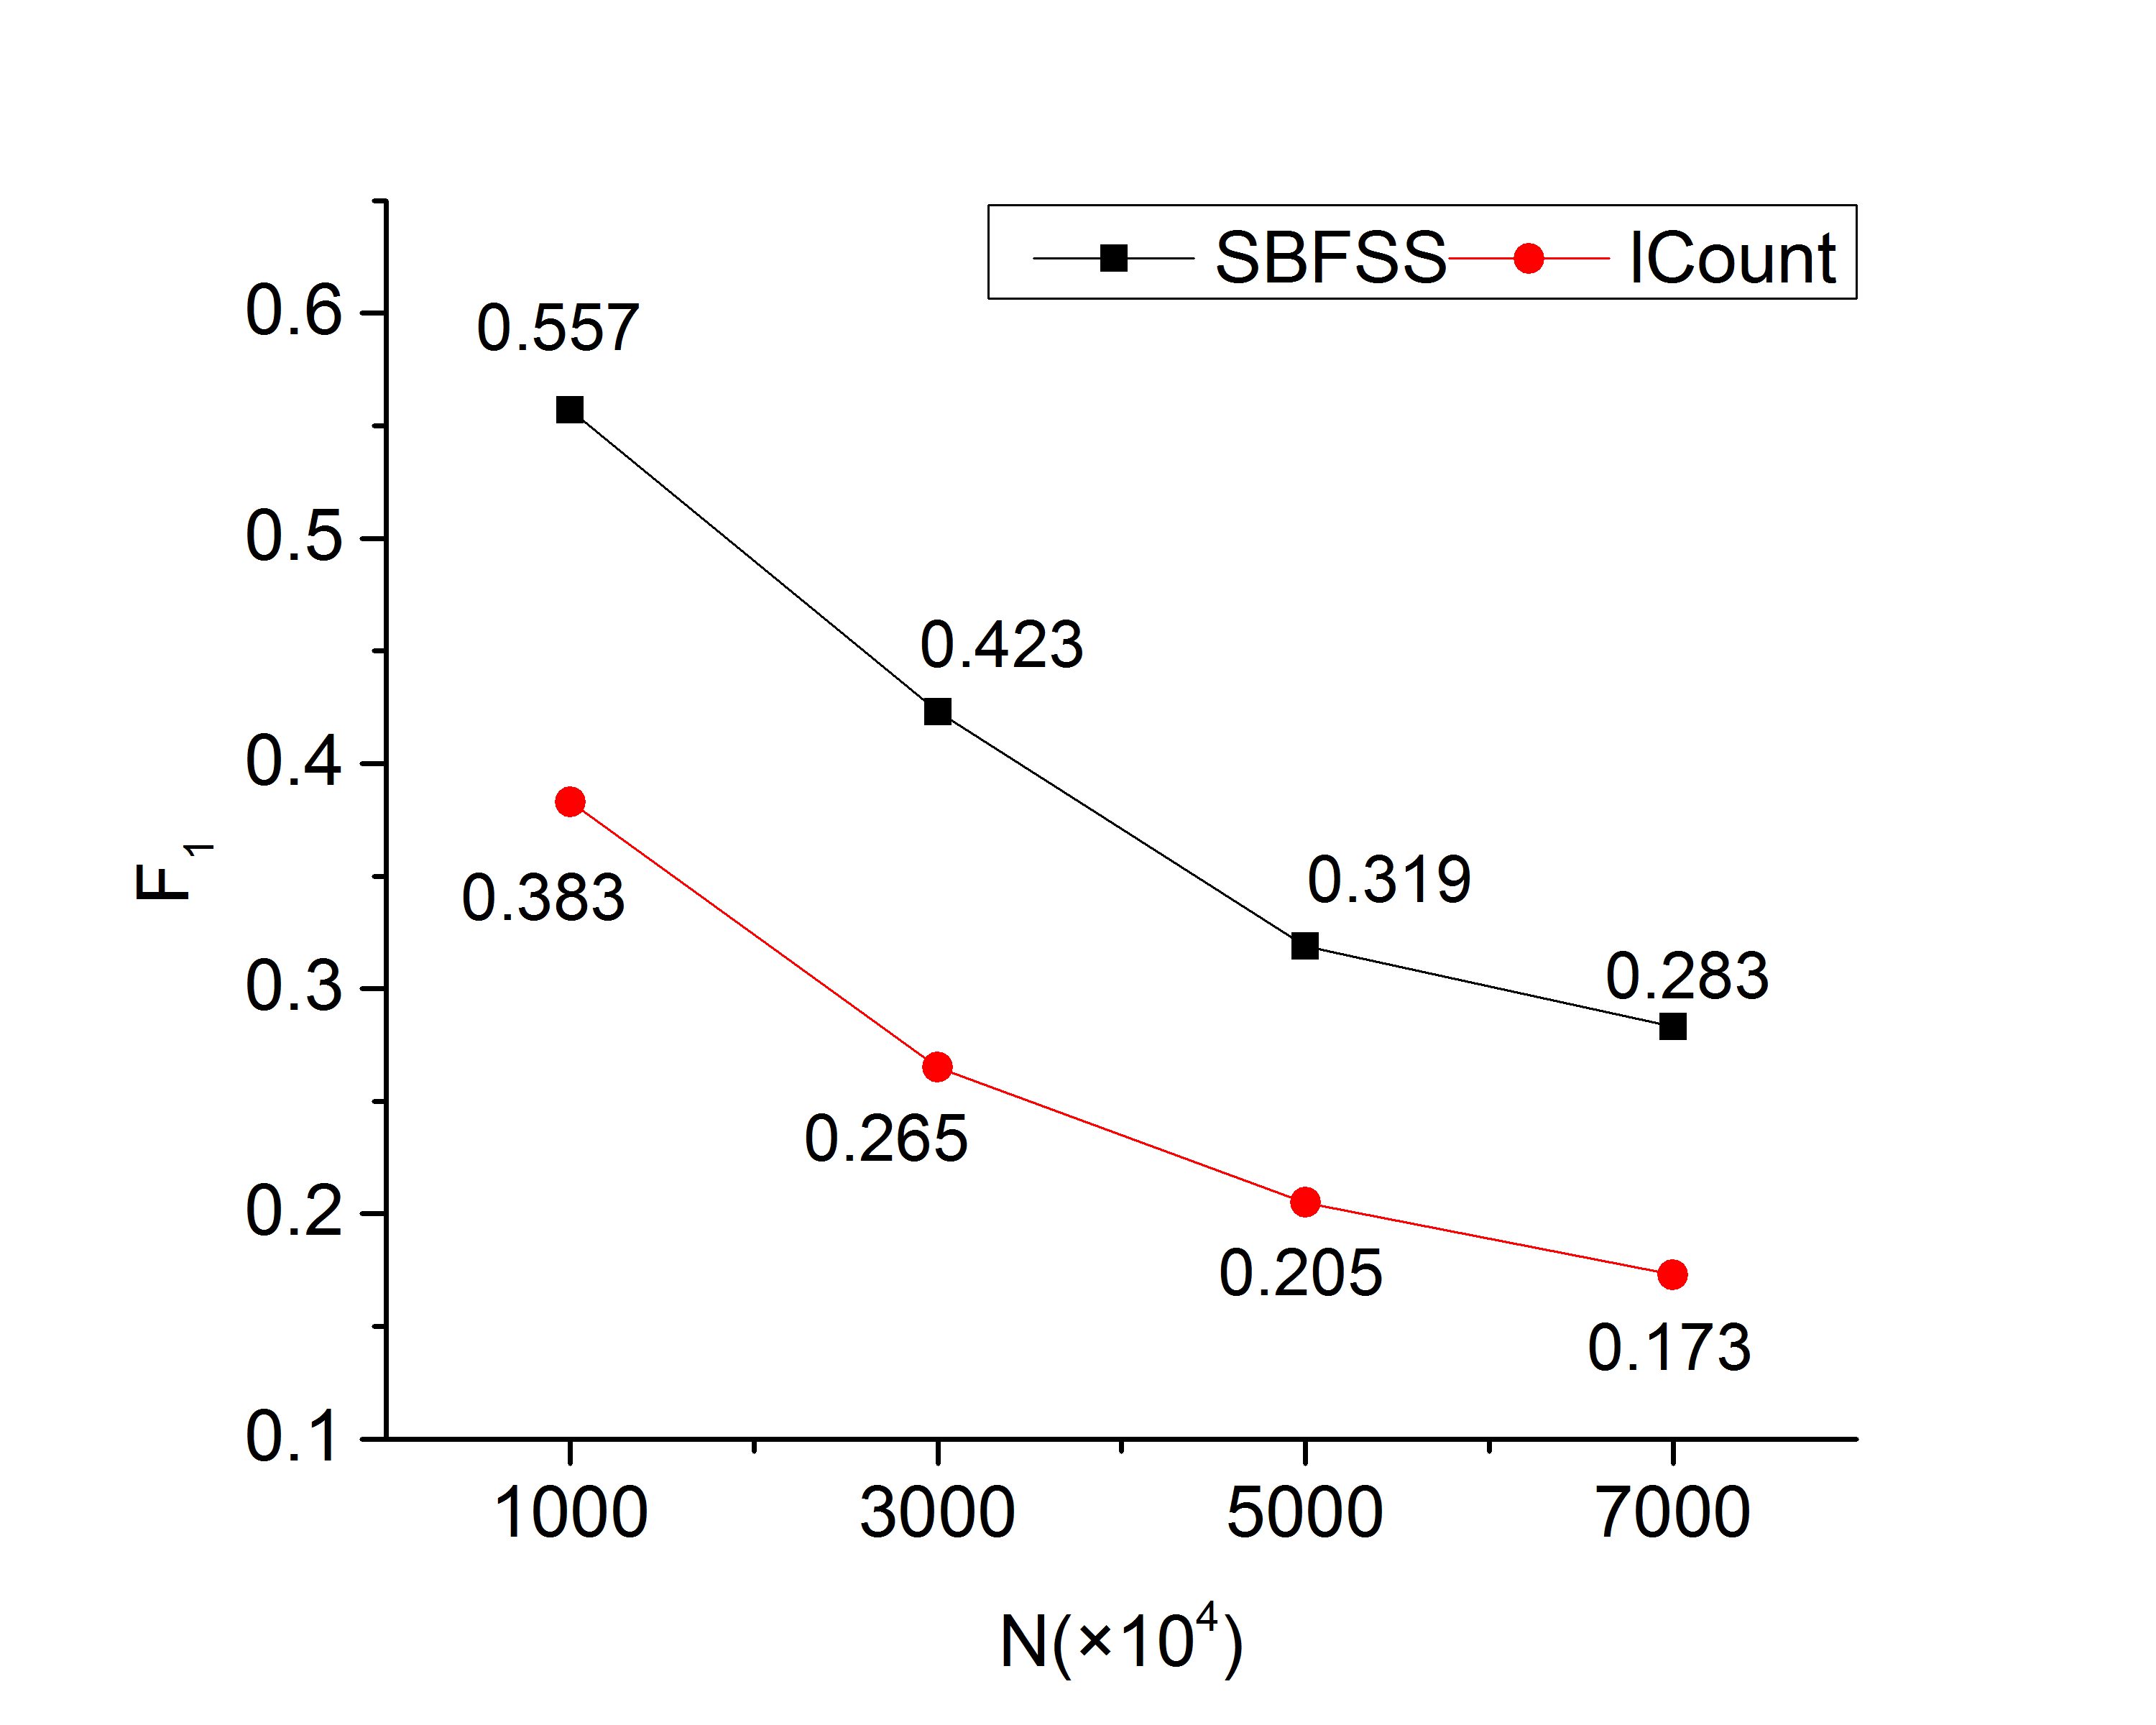
\includegraphics[width=1.95in]{png/001_54KB.png}}
	\end{minipage}
	\begin{minipage}{0.23\linewidth}
		\centering
		\subfloat[$s$=0.01, Space=72KB]{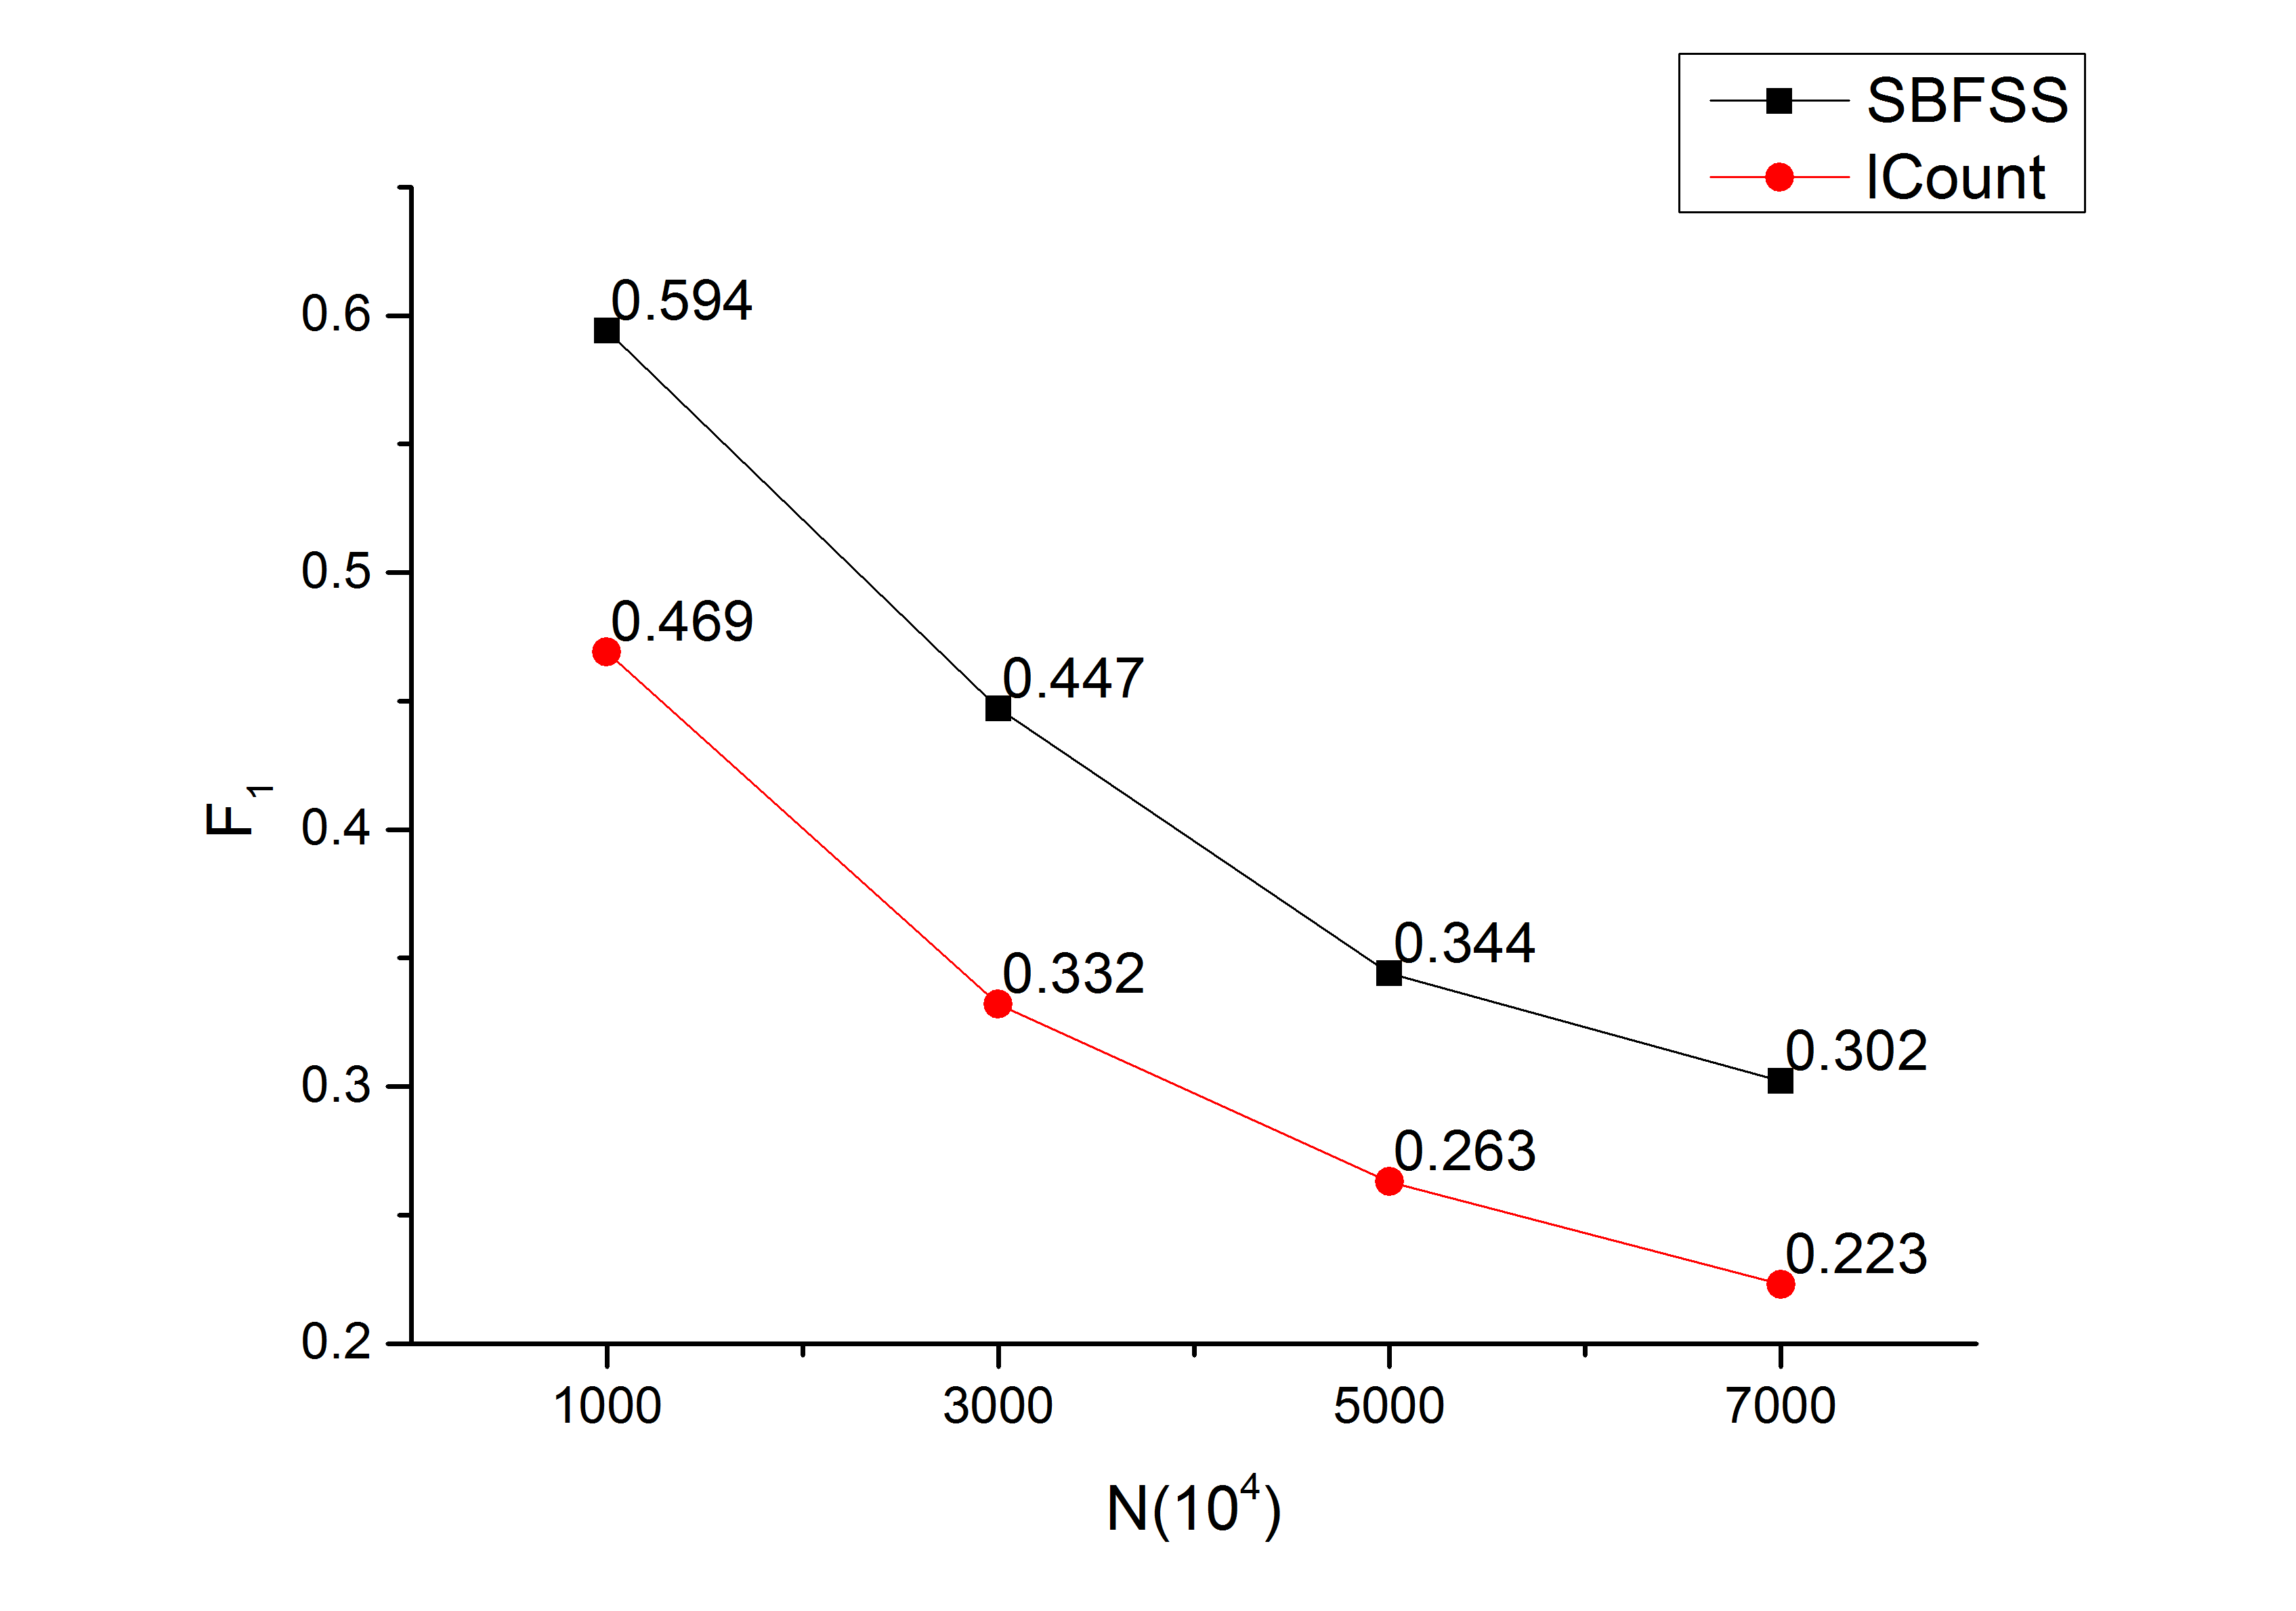
\includegraphics[width=1.95in]{png/001_72KB.png}}
	\end{minipage}
	\begin{minipage}{0.23\linewidth}
		\centering
		\subfloat[$s$=0.001, Space=54KB]{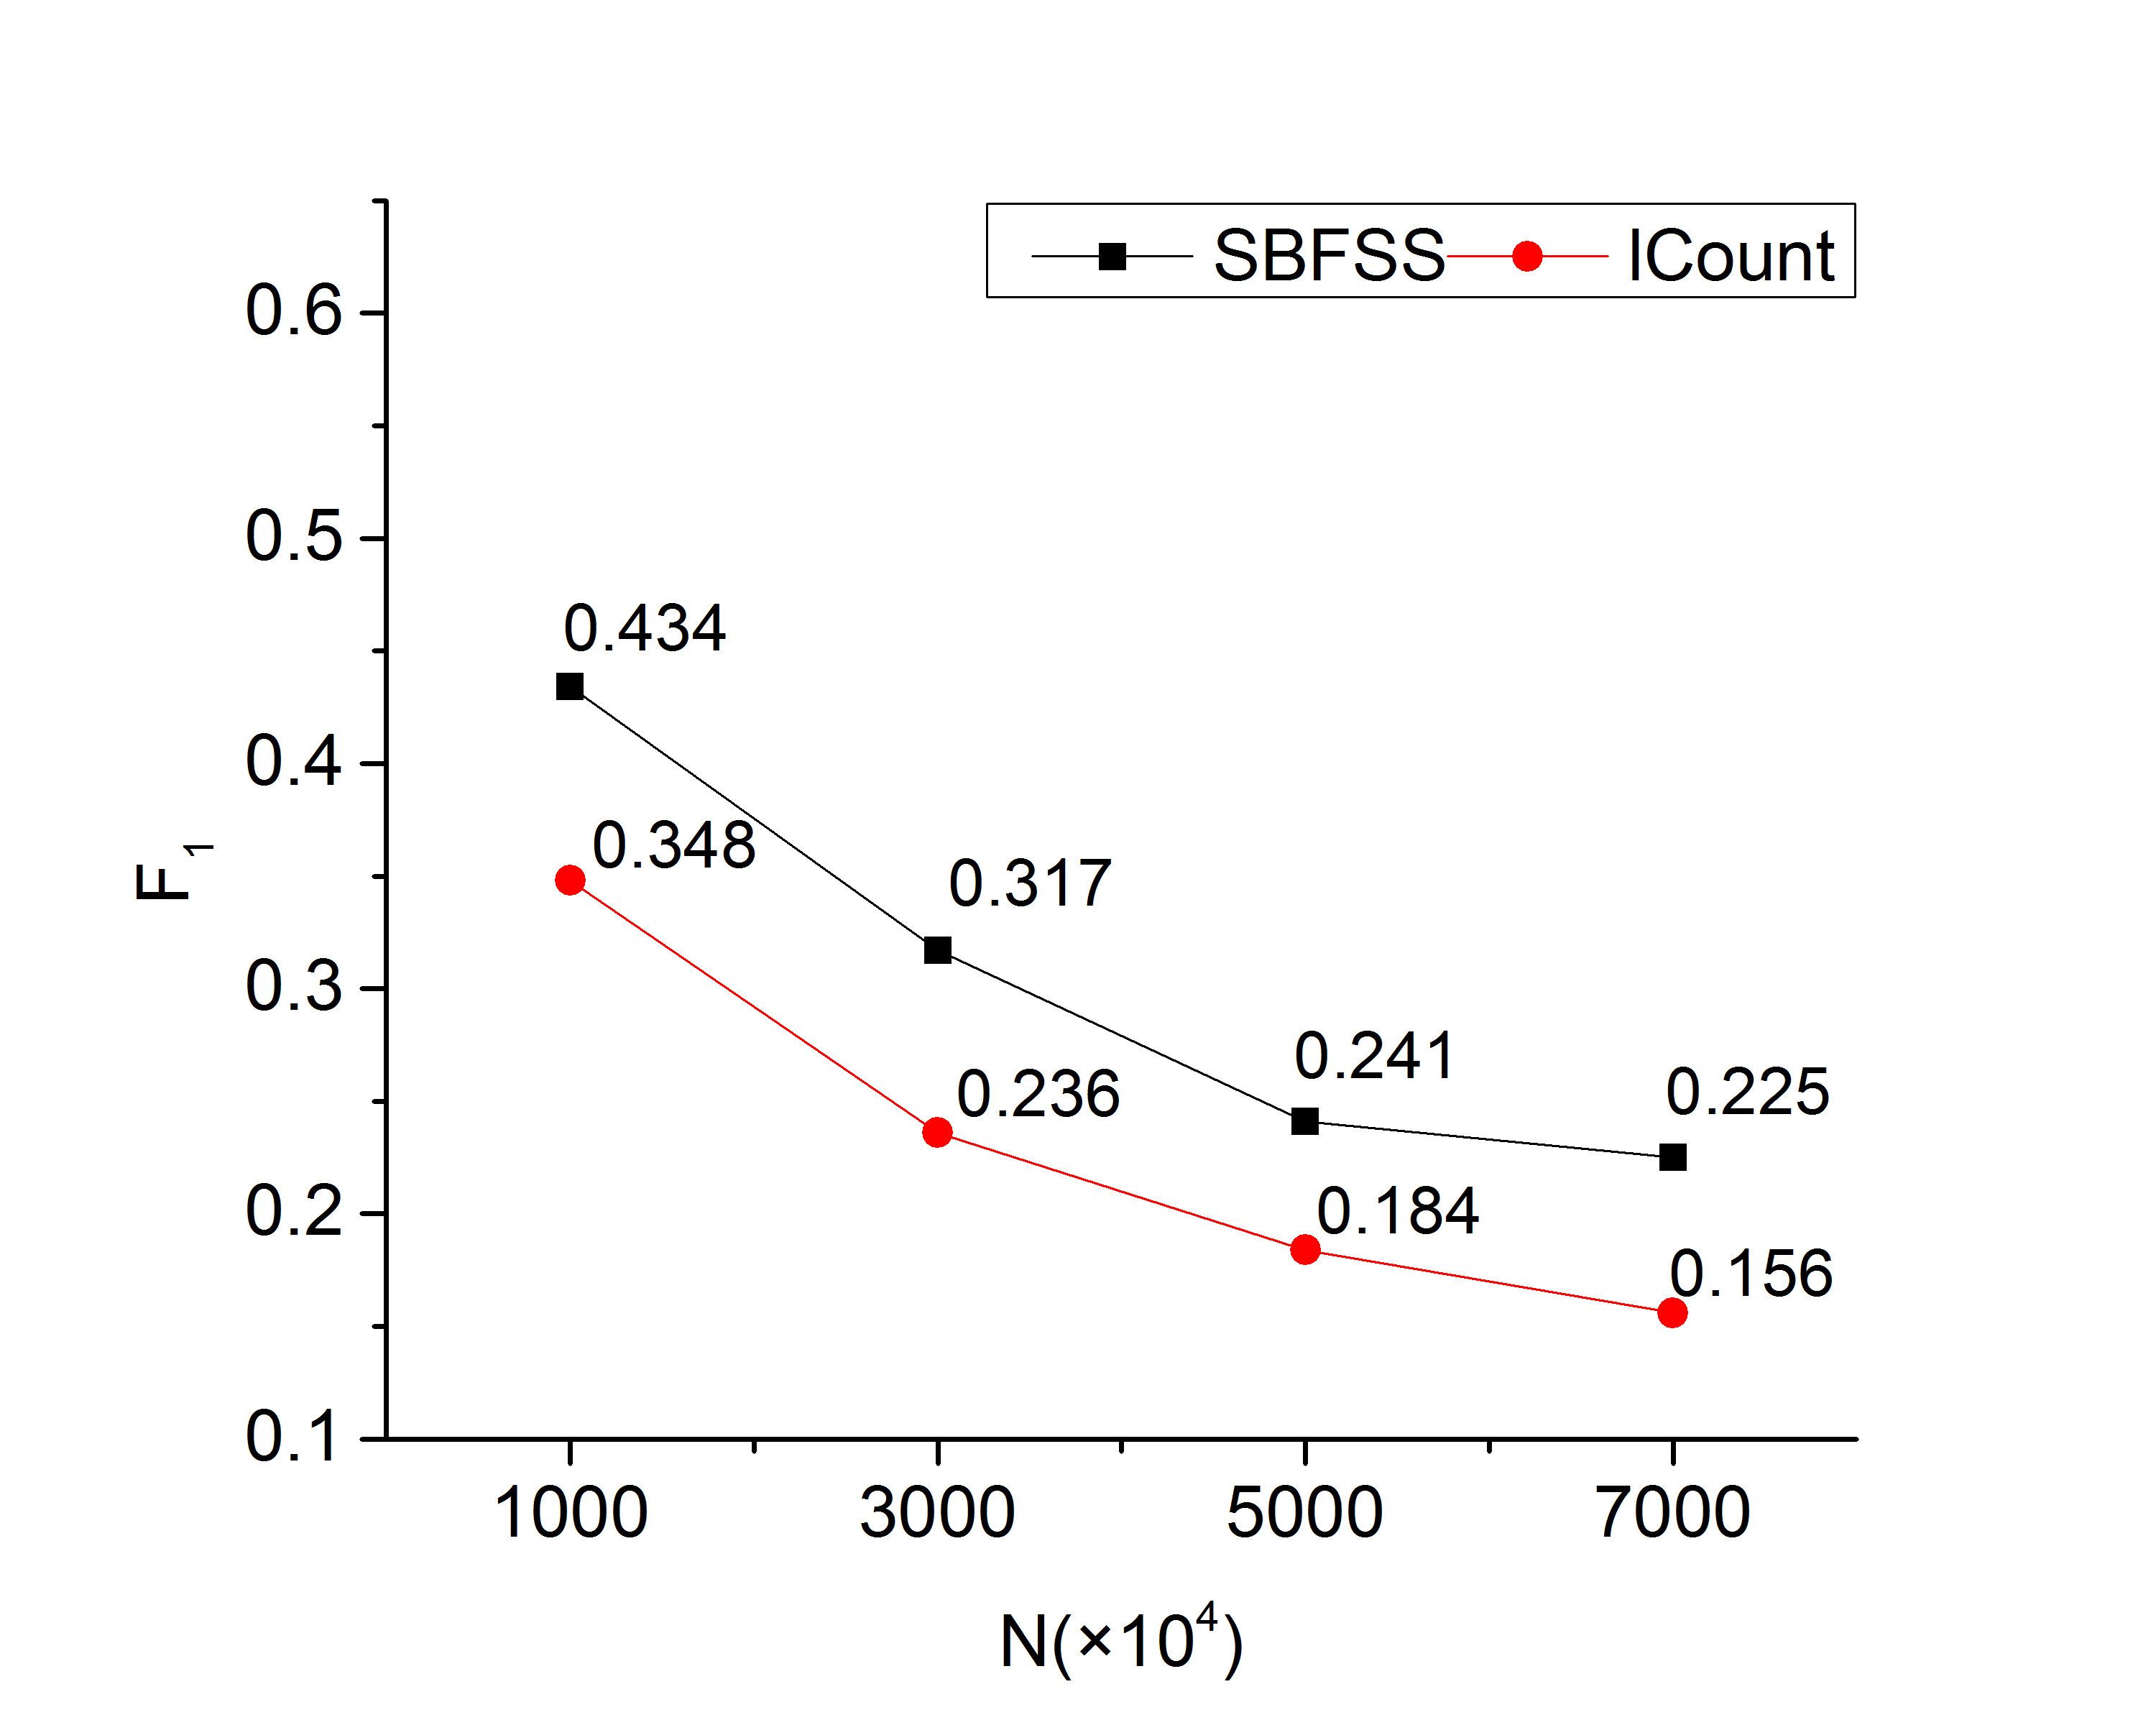
\includegraphics[width=1.95in]{png/0001_54KB.png}}
	\end{minipage}
	\begin{minipage}{0.23\linewidth}
		\centering
		\subfloat[$s$=0.001, Space=72KB]{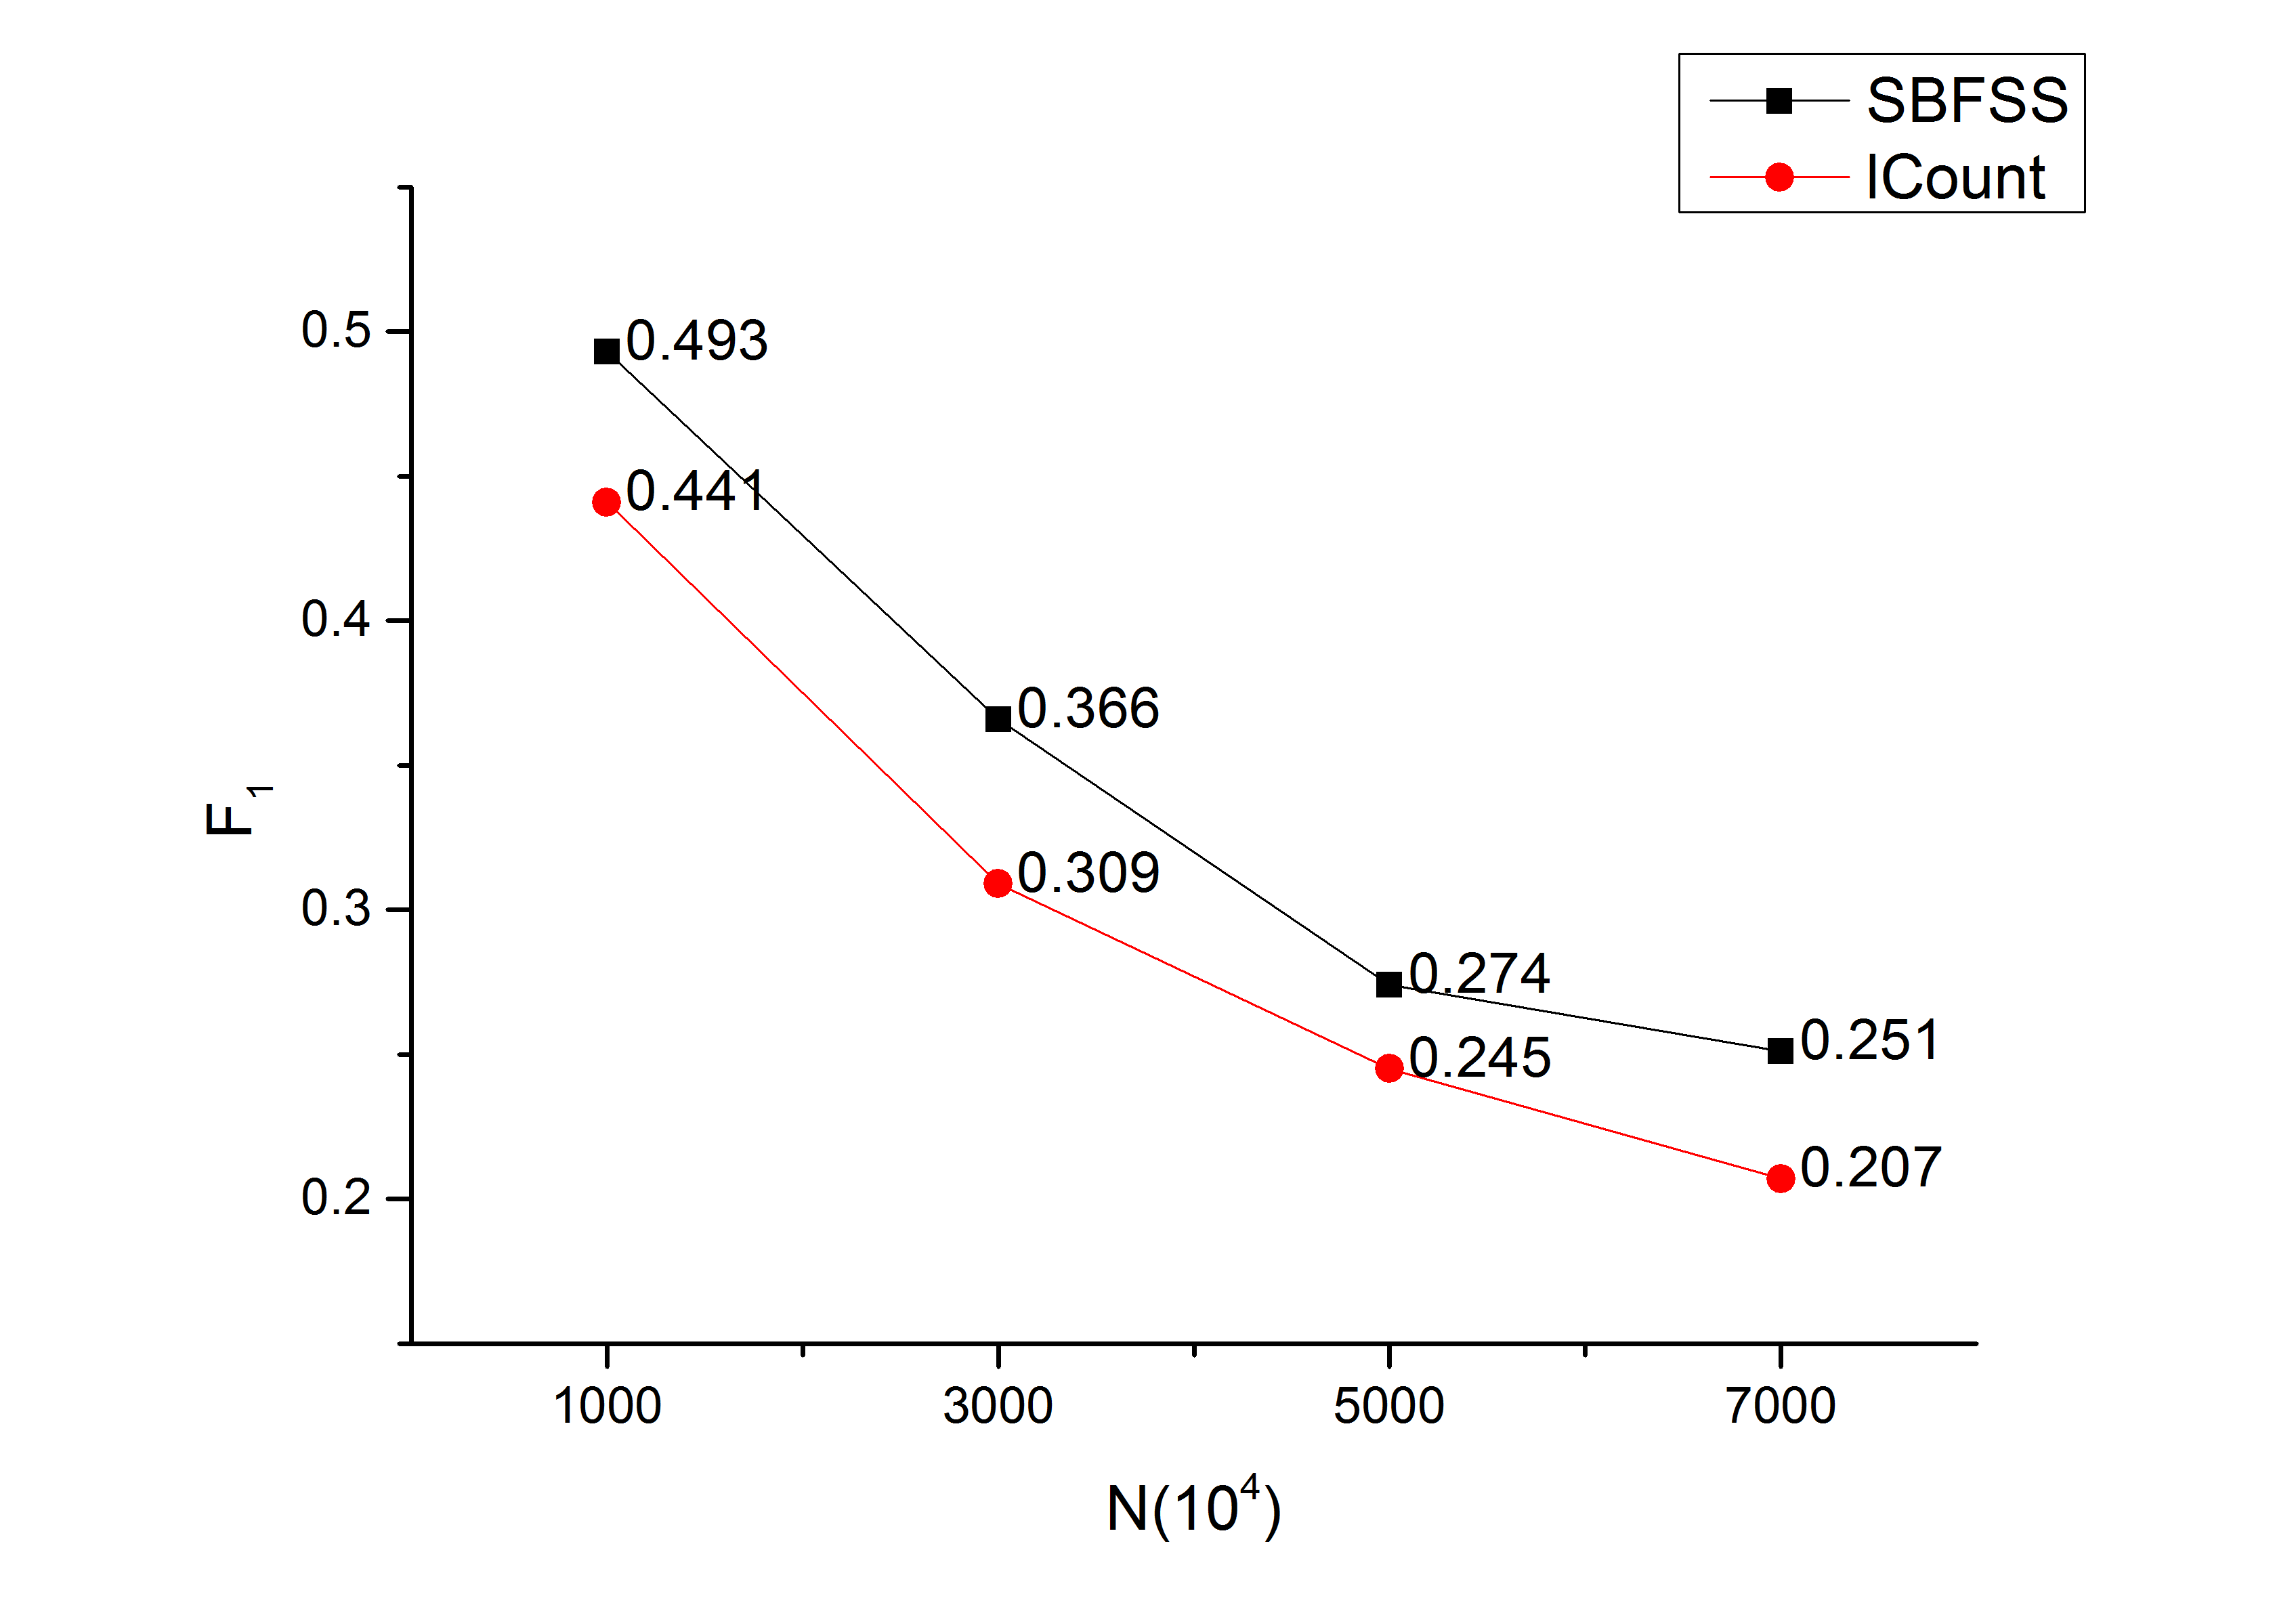
\includegraphics[width=1.95in]{png/0001_72KB.png}\label{subfig:f1_4}}
	\end{minipage}
	\caption{Performance Comparison of $F_1$ between \emph{SBFSS} and \emph{lCount} - Varying $s$ and Space}
	\label{fig:F1}
\end{figure*}
\subsection{Data Sets}
\textbf{Real Data.} For real data experiments, we used the dataset\footnote{http://ita.ee.lbl.gov/html/contrib/WorldCup.html}, denoted as $W$, which consists of all the requests made to the 1998 World Cup Web site between April 30, 1998 and July 26, 1998. We extracted $7\times10^7$ URLs in total, and the size of the alphabet is 89753.\par
\textbf{Synthetic Data.} We generated several synthetic Zipfian data sets with the Zipf parameter varying from 0.5, which is very slightly uniform, to 3.0, which is highly skewed, with a fixed increment of 0.5. The size of each data set, N, is $10^7$, and the size of the alphabet is $10^6$.
\subsection{Implementation Issues}
\textbf{\emph{BFSS} Implementation.} It is simple and straight forward to implement \emph{BFSS}: 1) hash each item into $H$ numbers, and set the corresponding $H$ bits to 1. 2) we maintain a min heap to index each counter in $D$, if the item is monitored, we simply increment its counter, otherwise if there exists an empty counter, we just insert a new counter into the heap, or we replace the top counter of the heap, at last we readjust the heap. 3) when a query comes, we just do as Algorithm \ref{alg:output} indicates.\par

Table \ref{tab:89753} lists the maximum value of $F(n)$ and the corresponding value of $n$ under various $K$ and $H$ combinations when $M$=89753, in which $H=\lfloor\frac{K}{M}\times ln2+\frac{1}{2}\rfloor$. The maximum value of $F(n)$ is 3909 when $\frac{K}{M}=3(K=269259)$ and $H=2$, and the upper bound of $E(\#FPs)$ can be confirmed once the value of $s$ is confirmed, which can be observed from Inequation \ref{eq:8}, for example $E(\#FPs)\leq 4909$ when $s=0.001$. Taking $E(\#FPs)$, update time and space consumption into consideration, we set $K=270000,400000,800000$ separately and $H=2$, and the corresponding maximum value of $F(n)$ is 3892, 2014 and 579 which decreases as $K$ increases, and this can be easily observed from the expression of $F(n)$.\par

\textbf{\emph{SBFSS} Implementation.} The only difference between \emph{BFSS} implementation and \emph{SBFSS} implementation is the implementation of \emph{BF} and \emph{SBF}. For \emph{SBF}, we generate a random number in each iteration, decrement the corresponding cell and $(P-1)$ cells adjacent to it by 1; this process is faster than generating $P$ random numbers for each item; although the processes of picking the $P$ cells are not independent, each cell has a probability of $P/k$ for being picked at each iteration. Our analysis still holds. Then we hash each incoming stream item to $H$ numbers, and set the corresponding $H$ cells to max. Taking the number of \emph{FNs}, the number of \emph{FPs}, update time and limited space we can use into consideration, we set $max=3, H=4$ and $P=1$.\par

\textbf{\emph{nCount} Implementation.} The basic idea of \emph{nCount} is to allocate each distinct item in $S$ a counter, we use a hash table to index these counters to speedup updating, and it is time consuming if we use a linked list or an array. When an item comes, we increment the corresponding counter using hash table. When a query comes, we traverse the hash table and output the low-frequency items. \par

\textbf{\emph{rCount} Implementation.} \emph{rCount} shares a similar idea with \emph{nCount}, however, unlike \emph{nCount}, \emph{rCount} uses Rabin's method \cite{rabin1981fingerprinting} to hash each item in $S$ to a 64-bit fingerprint, or it will consume too much space especially when the items are URLs. With this fingerprinting technique, there is a small chance that two different URLs are mapped to the same fingerprint. When an item comes, we first calculate its fingerprint and then increment the corresponding counter using hash table. When a query comes, we traverse the alphabet $A$ and calculate the fingerprint of each item in $A$, then we check the corresponding counter and output it if it is a low-frequency item.\par

\textbf{\emph{lCount} Implementation.} \emph{lCount} maintains a limited and fixed space, like \emph{rCount}, \emph{lCount} uses Rabin's method in order to adjust the space consumption through the maximum number of counters \emph{lCount} can maintain. In addition, we use a max heap to index the counters in \emph{lCount}. When an item comes, if there exists an empty counter, we insert a new counter into the heap, otherwise we replace the top counter of the heap, i.e. the counter with the maximum value, and set the value of the new counter to 1, at last we readjust the heap. When a query comes, we traverse the alphabet $A$ and calculate the fingerprint of each item in $A$, then we check if the corresponding counter exists in the heap and output it if it is a low-frequency item.\par


\begin{figure}
	\centering
	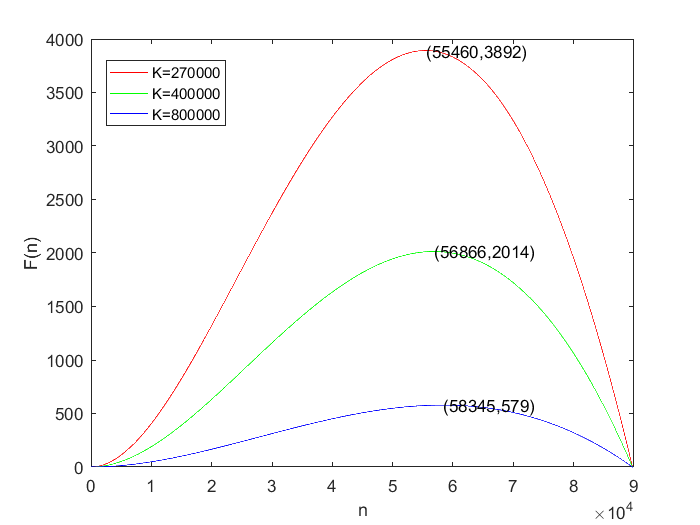
\includegraphics[width=3in]{png/F(n)-combine.png}
	\caption{The value of $F(n)$ when $M=89753$ and $H=2$ - Varying $K$}
	\label{fig:F(n)}
\end{figure}

\subsection{Performance of BFSS}
The query issued for \emph{BFSS}, \emph{nCount} and \emph{rCount} was to find all items whose frequency is no more than $\frac{N}{s}(s=1\%,0.2\%,0.1\%)$.\par
The results comparing the recall, precision, $F_1$ and space used by \emph{BFSS}, \emph{nCount} and \emph{rCount} are summarized in Fig. \ref{fig:performance comparison of BFSS}. The value of $N$ was varied from $10^7$ to $7\times 10^7$, and we set $K=400000,H=2$, in addition, we set the error parameter $\epsilon=s$, since our results showed that this was sufficient to give high accuracy in practice. Obviously, the recalls achieved by \emph{BFSS} and \emph{nCount} were constant at 1 for all values of $N$ and $s$, however, due to hash collisions, \emph{rCount} may neglect a few low-frequency items, as is clear from Fig. \ref{subfig:0001_recall}. From Fig. \ref{subfig:001_precison}, Fig. \ref{subfig:0002_precison} and Fig, \ref{subfig:0001_precison}, we observe that the precision of \emph{BFSS} decreased as the value of $N$ increased, in fact, as we discussed before, the value of $F(n)$ increases as the value of $n$ increases unitil $F(n)$ reaches its maximum value then the value of $F(n)$ decreases as the value of $n$ increases, which means the precision of \emph{BFSS} presented ealier decrease and later increase trend as the value of $N$ increased with high probability. Fig. \ref{fig:F(n)} shows the value of $F(n)$ when $M=89753$ and $H=2$ varying the value of $K$ from which we can observe that the value of $F(n)$ increases firstly and reduces at last, when $K=400000$, the maximum value of $F(n)$ is 2014 and the corresponding value of $n$ is 56866, therefore the maximum value of $E(\#FPs)$ is $2014+\frac{1}{s}$. The precision of \emph{rCount} increased as the value of $N$ increased because only the items not appearing in $S$ may become false positives, and the number of these items decreased with the increasing of $N$. In addition, the precision of \emph{nCount} remained unchanged at 1 because \emph{nCount} just kept a counter for each item in $S$. Being concerned with both precision and recall, we calculated the values of $F_1$ of these algorithms based on the precisions and recalls as Fig. \ref{subfig:001_f1}, Fig. \ref{subfig:0002_f1} and Fig. \ref{subfig:0001_f1} show, and \emph{BFSS} outperformed \emph{rCount} except when $N=7\times 10^7$. The advantage of \emph{BFSS} is evident in Fig. \ref{subfig:001_space}, Fig. \ref{subfig:0002_space} and Fig. \ref{subfig:0001_space}, which show that \emph{BFSS} achieved a greate reduction in space consumption, more specifically, when $s=0.1\%$, \emph{BFSS} achieved a space reduction by a factor of 5.7 to 14.2 compared with \emph{nCount} and a space reduction by a factor of 2.2 to 5.5 compared with \emph{rCount}, when $s=0.2\%$, \emph{BFSS} achieved a space reduction by a factor of 10.0 to 24.9 compared with \emph{nCount} and a space reduction by a factor of 3.9 to 9.6 compared with \emph{rCount}, when $s=1\%$, \emph{BFSS} achieved a space reduction by a factor of 18.2 to 45.2 compared with \emph{nCount} and a space reduction by a factor of 7.0 to 17.4 compared with \emph{rCount}. In addition, the space used by \emph{nCount} and \emph{rCount} increased rapidly as the value of $N$ increased since more counters were needed, however, the space used by \emph{BFSS} was stable because the space complexity of \emph{BFSS} is not ralated to the value of $N$, and the minor difference between the space used by \emph{BFSS} as the value of $N$ increased existed in the space used by $D$.\par
Table \ref{tab:bfss} shows the precision of \emph{BFSS} with different parameter settings, and the recall of \emph{BFSS} was constant at 1, which has been proved theoretically and practically, so we don't list here. We neglect the minor difference between the space used by \emph{BFSS} as the value of $N$ increased. The precision increased as the value of $K$ increased, in fact, from Fig. \ref{fig:F(n)}, we notice that the value of $F(n)$ decreases as the value of $K$ increases, therefore the value of $E(\#FPs)$ decreases as the value of $K$ increases too. Besides, once the values of $K$ and $N$ were confirmed the precision was almost confirmed too, which means the values of $s$ and $\epsilon$ had little affection on the precison and most of \emph{FPs} were caused by \emph{BF}.\par
From above, \emph{BFSS} achieved high precision and one hundred percent recall using much less space compared with \emph{nCount} and \emph{rCount}, in fact, we can give the maximum expected value of $E(\#FPs)$ theoretically. Besides, the space consumed by \emph{BFSS} was stable as the value of $N$ increased while the space consumed by \emph{nCount} and \emph{rCount} increased rapidly, which makes \emph{BFSS} more scalable than \emph{nCount} and \emph{rCount}.
\subsection{Distribution estimation}
Table \ref{tab:distribution} shows the estimation of the distribution of the real data when $N$ was $7\times10^7$, and we have two observations. First, the estimated results given by our method is precise enough, and nearly no difference exists between the estimated results and the real results, as is clear from the table. Another interesting obervation is that the most frequent one percent of the items in $W$ occupied more than seventy percent of the number of the items in $W$, which means most people were interested in a few webpages and most webpages were browsed only a few times, and from table \ref{tab:distribution}, we can see that ninety-nine percent of the items in $W$ occupied no more than thirty percent of the number of the items in $W$, in fact, about thirty-two percent of the items in $W$ were browsed only once, which is realy a ``long tail''.

\begin{table}
	\caption{Distribution Estimation of $W$.}
	\centering
	\begin{tabular}{|c|c|c|c|}
    \hline
    $s$&$>1\%$&$>0.55\%$&$>0.1\%$\\
    \hline
    estimated percentage of the items&0.027\%&0.22\%&1.1\%\\
    \hline
    estimated percentage of the frequencies&6.0\%&36\%&72\%\\
    \hline
    true percentage of the items&0.028\%&0.23\%&1.1\%\\
    \hline
    true percentage of the frequencies&6.0\%&36\%&72\%\\
    \hline
	\end{tabular}
	\label{tab:distribution}
\end{table}

\subsection{Performance of SBFSS}
As mentioned before, when the total space is limited, the space left for the Bloom filter is limited as well, and it may cause many \emph{FPs} when the space is small. Table \ref{tab:sbfss} shows the performance comparison between \emph{SBFSS} and \emph{lCount} when the space was limited. When $s$ was 0.01, \emph{SBFSS} outperformed \emph{lCount} in both precision and recall, and we can see that the precision of \emph{SBFSS} was stable and constant at 1 for most values of $N$, and the precision of \emph{lCount} increased with the increasing of $N$ the reason of which is much like \emph{rCount}. In addition, the recalls of \emph{SBFSS} and \emph{lCount} decreased with $N$ since the space was limited and the information we could maintain was limited too, which directly caused the decreasing of the recalls. When $s$ was 0.001, the rules of how the precisons and recalls changed was similar to the case when $s$ was 0.01, and we can find that \emph{SBFSS} still maintained high accuracy, however, the general performance of \emph{SBFSS} was not as good as the case when $s$ was 0.01 because much more space could be allocated to \emph{SBF} when $s$ was smaller. Another interesting observation is that \emph{SBFSS} performed better when the limited space is small, which can be clearly seen from Fig. \ref{fig:F1}, which shows the comparison of the $F_1$ between \emph{SBFSS} and \emph{lCount}. We can observe that when $s$ was confirmed, the smaller the space available was, the larger the gap between the $F_1$ was, and this obervation proves the efficiency of \emph{SBFSS}.
% An example of a floating figure using the graphicx package.
% Note that \label must occur AFTER (or within) \caption.
% For figures, \caption should occur after the \includegraphics.
% Note that IEEEtran v1.7 and later has special internal code that
% is designed to preserve the operation of \label within \caption
% even when the captionsoff option is in effect. However, because
% of issues like this, it may be the safest practice to put all your
% \label just after \caption rather than within \caption{}.
%
% Reminder: the "draftcls" or "draftclsnofoot", not "draft", class
% option should be used if it is desired that the figures are to be
% displayed while in draft mode.
%
%\begin{figure}[!t]
%\centering
%\includegraphics[width=2.5in]{myfigure}
% where an .eps filename suffix will be assumed under latex, 
% and a .pdf suffix will be assumed for pdflatex; or what has been declared
% via \DeclareGraphicsExtensions.
%\caption{Simulation Results}
%\label{fig_sim}
%\end{figure}

% Note that IEEE typically puts floats only at the top, even when this
% results in a large percentage of a column being occupied by floats.


% An example of a double column floating figure using two subfigures.
% (The subfig.sty package must be loaded for this to work.)
% The subfigure \label commands are set within each subfloat command, the
% \label for the overall figure must come after \caption.
% \hfil must be used as a separator to get equal spacing.
% The subfigure.sty package works much the same way, except \subfigure is
% used instead of \subfloat.
%
%\begin{figure*}[!t]
%\centerline{\subfloat[Case I]\includegraphics[width=2.5in]{subfigcase1}%
%\label{fig_first_case}}
%\hfil
%\subfloat[Case II]{\includegraphics[width=2.5in]{subfigcase2}%
%\label{fig_second_case}}}
%\caption{Simulation results}
%\label{fig_sim}
%\end{figure*}
%
% Note that often IEEE papers with subfigures do not employ subfigure
% captions (using the optional argument to \subfloat), but instead will
% reference/describe all of them (a), (b), etc., within the main caption.


% An example of a floating table. Note that, for IEEE style tables, the 
% \caption command should come BEFORE the table. Table text will default to
% \footnotesize as IEEE normally uses this smaller font for tables.
% The \label must come after \caption as always.
%
%\begin{table}[!t]
%% increase table row spacing, adjust to taste
%\renewcommand{\arraystretch}{1.3}
% if using array.sty, it might be a good idea to tweak the value of
% \extrarowheight as needed to properly center the text within the cells
%\caption{An Example of a Table}
%\label{table_example}
%\centering
%% Some packages, such as MDW tools, offer better commands for making tables
%% than the plain LaTeX2e tabular which is used here.
%\begin{tabular}{|c||c|}
%\hline
%One & Two\\
%\hline
%Three & Four\\
%\hline
%\end{tabular}
%\end{table}


% Note that IEEE does not put floats in the very first column - or typically
% anywhere on the first page for that matter. Also, in-text middle ("here")
% positioning is not used. Most IEEE journals/conferences use top floats
% exclusively. Note that, LaTeX2e, unlike IEEE journals/conferences, places
% footnotes above bottom floats. This can be corrected via the \fnbelowfloat
% command of the stfloats package.


\section{Conclusion}
Low-frequency items in data streams contain much useful information which can be widely used in commercial decision-making, data analysis, etc., and locating them is the first step. We present \emph{BFSS}, an effective and space efficient algorithm that aims to solve the problem \emph{$s$-BLFE} approximately. \emph{BFSS} can output all low-frequency items and a few frequent items, the number of which can be theoretically bounded. The experimental results show the recall of \emph{BFSS} was constant at 1 and the precision was above 0.95 using a small space. When the memory is limited and small, in which case \emph{BFSS} can not guarantee high precision, we propose \emph{SBFSS} which can guarantee . \par
The future directions of our work can be, but are not limited to: 1) output low-frequency items along with their approximate frequencies, and this can be achieved based on the data structure of the \emph{Count-Min Sketch} algorithm as we discussed before. 2) handle sliding window queries. 3) support both insertion and deletion of items. 4) find low-frequency item sets. In fact, like frequent items, there are many work can be done towards low-frequency items, however, due to the special features of them, we still have a long and tough way to go and we just take a small step forward.






% conference papers do not normally have an appendix


% use section* for acknowledgement
\section*{Acknowledgment}


The authors would like to thank...





% trigger a \newpage just before the given reference
% number - used to balance the columns on the last page
% adjust value as needed - may need to be readjusted if
% the document is modified later
%\IEEEtriggeratref{8}
% The "triggered" command can be changed if desired:
%\IEEEtriggercmd{\enlargethispage{-5in}}

% references section

% can use a bibliography generated by BibTeX as a .bbl file
% BibTeX documentation can be easily obtained at:
% http://www.ctan.org/tex-archive/biblio/bibtex/contrib/doc/
% The IEEEtran BibTeX style support page is at:
% http://www.michaelshell.org/tex/ieeetran/bibtex/
%\bibliographystyle{IEEEtran}
% argument is your BibTeX string definitions and bibliography database(s)
%\bibliography{IEEEabrv,../bib/paper}
%
% <OR> manually copy in the resultant .bbl file
% set second argument of \begin to the number of references
% (used to reserve space for the reference number labels box)



\bibliographystyle{./bibtex/IEEEtran}
\bibliography{./bibtex/IEEEabrv,./bibtex/IEEEexample}




% that's all folks
\end{document}


